\documentclass[a4paper,12pt,oneside,openright,final,oldfontcommands]{memoir}
\usepackage[table]{xcolor}
\usepackage{graphicx}
\usepackage[latin1]{inputenc}
\usepackage[ruled,vlined]{algorithm2e}
\usepackage{setspace}
\usepackage{url}
\usepackage{amsmath}
\usepackage{mathrsfs}
\usepackage{mathptmx}
\usepackage{amssymb}
\usepackage{bbm}
\usepackage{verbatim}
\usepackage{calc}
\usepackage{multirow}
\usepackage{page}
\usepackage{names}
\usepackage{pbox}
\usepackage{subcaption}
\usepackage{epstopdf}
\usepackage[portuges]{babel}
\usepackage[
    a4paper,
    portuguese,
    bookmarks=true,
    bookmarksnumbered=true,
    linktocpage,
    ]{hyperref}
\usepackage{memhfixc}
\usepackage{listings}
\usepackage{marvosym}
\usepackage{pgf}
\usepackage{indentfirst}
\usepackage{tikz}
\usetikzlibrary{arrows,automata,positioning,trees,shapes}
\usepackage{mdframed}
\usepackage[T1]{fontenc}
\usepackage{tabu}

\setlrmarginsandblock{3cm}{2cm}{*}
\setulmarginsandblock{3cm}{3cm}{*}
\setheaderspaces{2cm}{*}{*}

\checkandfixthelayout

\makeheadrule{myheadings}{\textwidth}{\normalrulethickness}
\makeoddhead{myheadings}{\textsc{\leftmark}}{}{\thepage}	%

\copypagestyle{contents}{myheadings}
\makeoddhead{contents}{\textsc{\contentsname}}{}{\thepage}

\copypagestyle{bibliography}{myheadings}
\makeoddhead{bibliography}{\textsc{\bibname}}{}{\thepage}

\makeatletter

\def\mychaptermark#1{%
	\markboth{%
	\ifnum \c@secnumdepth >\m@ne
		\if@mainmatter
			\thechapter. \ %
		\fi
	\fi
	#1}{}}%

\def\mysectionmark#1{%
\markright{%
	\ifnum \c@secnumdepth > \z@
		\thesection. \ %
	\fi
	#1}}%

\makeatother

\maxsecnumdepth{subsubsection}

\newcommand{\tableformat}{\small\centering}
\newcommand{\figureformat}{\centering}

\renewcommand{\labelenumi}{\alph{enumi})}
\renewcommand{\labelenumii}{\arabic{enumii}.}

\setcounter{tocdepth}{2} %-- ajusta produndidade do indice

\let\Chapter\chapter
\def\chapter{\addtocontents{lol}{\protect\addvspace{10pt}}\Chapter}

\renewcommand{\lstlistingname}{Algoritmo}
\renewcommand{\lstlistlistingname}{Lista de Algoritmos}

\lstset{
  numbers=left,
  stepnumber=1,
  firstnumber=1,
  numberstyle=\tiny,
  extendedchars=true,
  breaklines=true,
  frame=tb,
  basicstyle=\footnotesize,
  stringstyle=\ttfamily,
  showstringspaces=false,
  captionpos=b,
  breakautoindent=truem
  language=C,
  numbersep=5pt,
  tabsize=2,
  morekeywords={assert,enquanto,se,fim,entao,senao,retorne,faca,assume,Passo,for,int,long, unsigned,while}
}

\makeatletter
\renewcommand\l@lstlisting[2]{\@dottedtocline{1}{0cm}{0.95cm}{#1}{#2}}
\makeatother

\newcolumntype{P}[1]{>{\centering\arraybackslash}p{#1}}

\usepackage{parskip}
\setlength{\parindent}{35pt}


\hyphenation{matema-ticamente moni-torar operacio-nal ESBMC bi-bli-o-te-ca de-ter-mi-n�s-ti-cos mul-ti-pa-ra-dig-mas}

\begin{document}

\newtheorem{definition}{Defini��o}[chapter]
\newtheorem{lemma}{Lemma}[chapter]

\newtheorem{fact}{Fact}[chapter]

\newtheorem{example}{Example}[chapter]

% -- Titulo e Descricao ------------------------------------------------------
\newcommand{\tittese}{%
	\textsf{\bfseries\Large Meu Titulo Vem Aqui \\
	\vspace{0.8ex}
        }}

\newcommand{\descrtese}{%
\hspace{\stretch{1}}\parbox{0.51\textwidth}{%
Disserta��o apresentada ao Programa de P\'os-Gradua\c{c}\~ao em Engenharia El�trica, como requisito parcial
para obten\c{c}\~ao do T\'{\i}tulo de Mestre em Engenharia El�trica. \'Area de concentra\c{c}\~ao: Automa��o e Controle.
}}

% -- Capa ---------------------------------------------------------------------

\frontmatter
%\doublespacing
%\singlespacing
\pagestyle{empty}

%{centering
\begin{center}

\includegraphics[bb=0 0 646 638,height=2.5cm]{figures/ufam.png}

\textsf{\large%
Universidade Federal do Amazonas\\
Faculdade de Tecnologia\\
Programa de P\'os-Gradua\c{c}\~ao em Engenharia El�trica}

\vspace*{4cm}
\vspace*{\stretch{1}}

\tittese

\vspace*{4cm}
\vspace*{\stretch{1}}

{\large Thiago Rodrigo F�lix Cavalcante}

\vspace*{3cm}
\vspace*{\stretch{1}}

Manaus -- Amazonas

Agosto de 2018
\end{center}

%}
%\cleardoublepage


% -- Contracapa ---------------------------------------------------------------

%{\singlespacing\centering
\begin{center}
{\large Thiago Rodrigo F�lix Cavalcante}

\vspace*{4cm}
\vspace*{\stretch{2}}

\tittese

\vspace*{2cm}
\vspace*{\stretch{1}}

\descrtese

\vspace*{2cm}
\vspace*{\stretch{1}}

Orientador: Prof. D.Sc. Eddie Batista de Lima Filho \\
\end{center}

%}
%\cleardoublepage


% -- Banca Examinadora --------------------------------------------------------

%{\singlespacing\centering

\begin{center}
{\large Thiago Rodrigo F�lix Cavalcante}

\vspace*{3cm}
%\vspace*{\stretch{2}}

\tittese

\vspace*{1cm}
%\vspace*{\stretch{1}}

%\descrtese

\vspace*{1cm}
%\vspace*{\stretch{1}}

Banca Examinadora
\vspace{2em}

Prof. D.Sc. Eddie Batista de Lima Filho -- Presidente e Orientador\\
TP Vision
\vspace{2em}

Prof. Ph.D. Lucas Carvalho Cordeiro -- Co-orientador\\
Escola de Ci�ncia da Computa��o -- UoM
\vspace{2em}

Prof. D.Sc. Raimundo da Silva Barreto \\
Instituto de Computa��o -- UFAM
\vspace{2em}

Prof. D.Sc. Renan Landau \\
Faculdade de Tecnologia -- UFAM
\vspace{2em}

%\vspace*{1cm}
\vspace*{\stretch{0.5}}

Manaus -- Amazonas

Agosto de 2018

\end{center}
%}
\cleardoublepage

\cleardoublepage

\vspace*{\stretch{2}}

\begin{flushright}
\textit{� minha fam�lia e minha noiva.}\hspace{1cm}
\end{flushright}

\vspace*{\stretch{1}}

\cleardoublepage

\chapter*{Agradecimentos}
\thispagestyle{empty}

Em primeiro lugar, agrade�o a Deus pelo dom da vida e por todas as conquistas alcan�adas. E o mais importante, agrade�o pelo Seu cuidado e Seu amor.

Agrade�o � minha esposa, J�ssica Alves, por todo amor, suporte, cuidado e carinho. Eu amo voc� e sei que voc� sempre est� ao meu lado. Voc� � o motivo de eu querer ir al�m.

Agrade�o � minha m�e, Francisca Silva, ao meu pai, Rubens Alves, e ao meu irm�o, Erick Alves, que me educaram e sempre me motivaram a ir al�m do que eu imaginava poder ir.

Agrade�o aos meus amigos de escola, Henrique Cavalcante, Juscelino Tanaka, Leandro Paes, Matheus Santos e Tayane Figueira, que apesar de tudo, sei que sempre torcem por mim; aos meus amigos da UFAM, Arllem Farias, Breno Linhares, Ciro Cativo, Helton Nogueira, Rosmael Miranda, Thiago Cavalcante e Weider Serruia, que foram meus companheiros durante os anos de gradua��o, mestrado e da vida; aos meus amigos do trabalho, do INDT e do SIDIA, em especial Allann Silva e Pablo Quiroga, por todo o apoio durante cada passo; e aos meus amigos da Igreja, em especial Labib Ismail, pelas risadas, conversas e lanches.

Agrade�o tamb�m aos meus orientadores, Prof. Eddie Lima Filho e Prof. Lucas Cordeiro, pela amizade, direcionamento, suporte, paci�ncia e conselhos. Saibam que me espelho em voc�s como profissional. Continuem procurando dar um caminho melhor a alunos atrav�s da educa��o.

\vspace*{3cm}
\cleardoublepage

\vspace*{1cm}
\vspace*{\stretch{1}}

\hspace{\stretch{1}}\parbox{0.5\textwidth}{
\begin{flushright}
\emph{``Porque dEle, e por meio dEle, e para Ele s�o todas as coisas. A Ele, pois, a gl�ria eternamente. Am�m!''.}
\end{flushright}
}
\vspace{2em}

\hspace{\stretch{1}}{\emph{Romanos 11:36}}

\vspace*{\stretch{1}}
\chapter*{Resumo}
\thispagestyle{empty}

Neste trabalho descrevemos uma abordagem para realizar s�ntese em sistemas de controle discreto com realimenta��o de estados com respeito a requisitos de performance a qual � baseada em t�cnicas de s�ntese indutiva guiada por contraexemplo (CEGIS). Nessa abordagem verifica-se um requisito de performance (\textit{e.g.} tempo de assentamento e m�ximo sobressinal) em um determinado sistema de controle com o objetivo de saber se satisfaz ao valor desejado para esse requisito, caso n�o satisfa�a, deve-se encontrar um sistema que satisfa�a ao requisito desejado, e nesse caso, redefine-se o controlador do sistema. Para gera��o do controlador, utilizamos uma t�cnica de aprendizagem onde a cada itera��o que a verifica��o do requisito n�o satisfa�a, aprende-se que esse controlador n�o nos serve. Na verifica��o desses requisitos de performance em sistemas de controle discreto, consideramos a fragilidade (\textit{erro de quantiza��o num�rica, arredondamento, efeitos de FWL, etc}) nos controladores utilizados. Essa abordagem � �til para auxiliar engenheiros de controle em seus projetos de sistemas de controle discreto, visto que essas fragilidades ocorrem durante a implementa��o em uma plataforma digital, e nesse caso, essa abordagem gera o sistema que satisfaz os requisitos desejados no projeto. Essa abordagem foi implementada dentro do DSVerifier que � uma ferramenta que emprega verifica��o de modelo limitada (e ilimitada) baseada em, teorias de m�dulo de satisfatibilidade. Nossa abordagem foi avaliada em um conjunto de \textit{benchmarks} cl�ssicos de sistemas de controle extra�dos da literatura, bem como em \textit{benchmarks} espec�ficos considerando diferentes autovalores e em diferentes configura��es. Os resultados experimentais mostram que a abordagem elaborada � eficaz para a s�ntese de requisitos de perfomance em sistemas de controles discreto com realimenta��o de estados, visto que considera problemas pr�ticos de implementa��o (efeitos FWL), diferentemente de outros m�todos que rotineiramente n�o consideram esses problemas.

\vspace*{\stretch{1}}

\noindent \textsf{Palavras-chave:} Sistemas de controle, Verifica��o de Parametros de Performance, Sintese.
%}

\cleardoublepage

\chapter*{Abstract}
\thispagestyle{empty}

In this work we describe an approach to perform synthesis in discrete control systems with state feedback over performance requirements which is based on counterexample-guided inductive synthesis techniques (CEGIS). In this approach there is a performance requirement (\textit{e.g.}, settling time and maximum overshoot) in a given control system in order to know if it satisfies the desired value for that requirement, if it does not satisfy, one must find a system that satisfies the desired requirement, in which case the system controller is reset. For the generation of the controller, we use a learning technique where each iteration that the verification of the requirement does not satisfy, we learn that this controller is not worthy. In the verification of these performance requirements in discrete control systems, we consider the fragility (numerical quantization error, round-offs, etc.) in the controllers used. This approach is useful for assisting control engineers in their discrete control systems projects, since such weaknesses occur during implementation on a digital platform, in which case this approach generates the system that meets the requirements desired in the design. This approach was implemented using DSVerifier which is a tool that employs bounded (and unbounded) model verification based on satisfiability module theories. Our approach was evaluated in a set of classical control system benchmarks extracted from the control literature, as well as in specific benchmarks considering different eigenvalues. The experimental results show that the elaborated approach is effective for the synthesis of perfomance requirements in discrete state feedback control systems since it considers practical implementation problems (FWL effects), unlike other methods that routinely do not consider these problems.

\vspace*{\stretch{1}}

\noindent \textsf{Keywords:} Control systems, Performance Requirement Verification, Synthesis.

\cleardoublepage


\pagestyle{contents}

\tableofcontents*
\cleardoublepage

\phantomsection
\addcontentsline{toc}{chapter}{\listfigurename}
\listoffigures*
\cleardoublepage

\phantomsection
\addcontentsline{toc}{chapter}{\listtablename}
\listoftables*
\cleardoublepage

%\lstlistoflistings
%\cleardoublepage

\chapter{Abrevia��es}
\label{appendix:abreviacao}

\noindent
\textbf{AD}       - \textit{\textbf{A}nal�gico \textbf{D}igital} \\
\textbf{ATS}      - \textit{\textbf{A}daptative \textbf{T}ransition \textbf{S}ystem} \\
\textbf{BDD}      - \textit{\textbf{B}anary \textbf{D}ecision \textbf{D}iagram} \\
\textbf{BIBO}     - \textit{\textbf{B}ounded \textbf{I}nput \textbf{B}ounded \textbf{O}utput} \\
\textbf{BMC}      - \textit{\textbf{B}ounded \textbf{M}odel \textbf{C}hecking} \\
\textbf{CEGIS}    - \textit{\textbf{C}ounter \textbf{E}xample \textbf{G}uided \textbf{I}nductive \textbf{S}ynthesis} \\
\textbf{CTL}      - \textit{\textbf{C}omputational \textbf{T}ree \textbf{L}ogic} \\
\textbf{DA}       - \textit{\textbf{D}igital \textbf{A}nal�gico} \\
\textbf{FSM}      - \textit{\textbf{F}inite \textbf{S}tate \textbf{M}achine} \\
\textbf{FWL}      - \textit{\textbf{F}inite \textbf{W}ord \textbf{L}ength} \\
\textbf{LQR}      - \textit{\textbf{L}inear \textbf{Q}uadratic \textbf{R}egulator} \\
\textbf{LTL}      - \textit{\textbf{L}inear \textbf{T}emporal \textbf{L}ogic} \\
\textbf{MAP}      - \textit{\textbf{M}ean \textbf{A}rterial \textbf{P}ressure} \\
\textbf{MDD}      - \textit{\textbf{M}ultiple \textbf{D}ecision \textbf{D}iagram} \\
\textbf{PSO}      - \textit{\textbf{P}article \textbf{S}warm \textbf{O}ptimization} \\
\textbf{PWA}      - \textit{\textbf{P}iece \textbf{W}ise \textbf{A}ffine} \\
\textbf{QPSO}     - \textit{\textbf{Q}uantic \textbf{P}article \textbf{S}warm \textbf{O}ptimization} \\
\textbf{RAM}      - \textit{\textbf{R}andom \textbf{A}ccess \textbf{M}emory} \\
\textbf{RCLF}     - \textit{\textbf{R}obust \textbf{C}ontrol \textbf{L}Lyapunov-like \textbf{F}unction} \\
\textbf{SDP}      - \textit{\textbf{S}emi \textbf{D}efinite \textbf{P}rogramming} \\
\textbf{SISO}     - \textit{\textbf{S}ingle \textbf{I}nput \textbf{S}ingle \textbf{O}utput} \\
\textbf{SMT}      - \textit{\textbf{S}atisfiability \textbf{M}odulo \textbf{T}heories} \\

\mainmatter
\pagestyle{myheadings}

\let\chaptermark=\mychaptermark
\let\sectionmark=\mysectionmark

\setcounter{secnumdepth}{2}

\chapter{Introdu��o}\label{chap-introduction}

Um sistema de controle digital consiste de sensores, sistema controlado, algoritmos de controle e atuadores, que juntos buscam manter o comportamento das vari�veis de uma planta (sistema controlado) sob controle, ou seja, garantem as respostas desejadas de estado estacion�rio e transit�rio~\cite{boyd1991linear}.
O desenvolvimento de controladores digitais � uma tarefa fundamental na engenharia de controle, uma vez que eles s�o rotineiramente usados para muitas aplica��es diferentes, que v�o desde a ind�stria at� no ramo aeroespacial~\cite{simons1994levers}.

A teoria de controle digital visa preservar algumas propriedades baseadas em modelos de tempo discreto, por exemplo, estabilidade e robustez, que s�o necess�rias para a opera��o correta de plantas reais atrav�s de um controlador digital. Controlar sistemas cont�nuos usando controladores digitais levanta problemas t�picos de sistemas h�bridos.
Al�m disso, arredondamento e quantiza��o de amostras e coeficientes em controladores digitais, devido a implementa��es de comprimento de palavras finitas (\textit{finite word length} - FWL), podem levar a \textit{overflow}, oscila��o de ciclo limite e sensibilidade a polos e zeros, o que pode causar instabilidade do sistema e degrada��o do desempenho~\cite{istepanian2012digital,BessaICF16,bessa2017formal}. De fato, esse tipo de sensibilidade � chamado de fragilidade~\cite{keel1997robust} e � importante para o projeto de sistemas de controle, uma vez que est� diretamente relacionado � sua robustez. Na literatura, existem alguns estudos relacionados que consideram perturba��es nas implementa��es de sistemas de controle; Yordanov et al. \cite{yordanov2012temporal} considera pequenas perturba��es nas entradas aplicadas em um sistema din�mico para a s�ntese de uma estrat�gia de controle de realimenta��o para um sistema de afinidade por partes (PWA) em tempo discreto a partir de uma especifica��o dada como uma f�rmula de l�gica linear temporal (LTL) sobre um conjunto de predicados lineares nas vari�veis de estado do sistema.

Algumas iniciativas que utilizam a verifica��o formal aplicada a sistemas de controle din�micos foram desenvolvidas nos �ltimos anos. Por exemplo, Bessa et al. \cite{bessa2017formal} apresentam um m�todo de verifica��o para determinar a estabilidade incerta do sistema linear em rela��o aos controladores digitais, levando em conta aspectos de implementa��o, enquanto Wang et al., ampliam as t�cnicas tradicionais de verifica��o para implementa��o de controladores digitais, com o objetivo de abordar a valida��o da robustez no modelo e no n�vel de c�digo. Abreu et al. \cite{abreu2016bounded} desenvolvem um m�todo para verificar filtros digitais relativos a \textit{overflow} e ru�do indesejado, que s�o causados por efeitos de quantiza��o e arredondamento, e Belta~\cite{belta2014formal} verificaram a estabilidade em sistemas din�micos. Al�m disso, Racchetti et al.\cite{racchetti2015verification} geraram sequ�ncias de teste a partir de diagramas temporais de especifica��es de \textit{software} e as executaram em tempo real, verificou-se parte de sua conformidade, salvou-se contornos de teste e analisou-os automaticamente atrav�s de um m�todo de verifica��o.
Nilsson et al.~\cite{nilsson2016correct} aplicam m�todos formais de controle de cruzeiro adaptativo e executa s�ntese de controlador que � correta por constru��o.

Em sistemas de controle, par�metros de resposta a degraus s�o comumente usados para especificar um elemento de controle, a fim de indicar que um sistema de controle de malha fechada � seguro em rela��o �s suas especifica��es de desempenho, ou seja, quando sua resposta ao degrau atende, por exemplo, especifica��es de tempo assentamento e sobressinal~\cite{franklin1998digital}.
 %
No entanto, existem alguns estudos relacionados que abordam par�metros de desempenho com m�todos formais.
Nesse sentido, Gross et al. apresentam uma abordagem para formalizar requisitos comuns de sistemas de controle de atitude de naves espaciais, onde os tempos de assentamento s�o verificados atrav�s de testes de hip�teses \cite{gross2017formal}; Jin et al. prop�em uma estrutura baseada em m�todos formais para capturar requisitos de modelos em malha fechada de sistemas de controle em escala industrial, incluindo tempo de assentamento e sobressinal \cite{jin2015mining}.
De fato, dado que perturba��es ou mudan�as em entradas pode levar a oscila��es transit�rias em sa�das, � importante que estes �ltimos estejam dentro da regi�o de assentamento, isto �, uma �rea especificando os desvios tolerados de uma dada refer�ncia, dentro de um tempo de assentamento especificado, e os sobressinais s�o menores do que um valor m�ximo requerido~\cite{jin2015mining}.

Tamb�m � importante refor�ar que os efeitos FWL realmente t�m um grande impacto no comportamento do sistema~\cite{istepanian2012digital}. Geralmente, os controladores s�o fortemente influenciados por ligeira imprecis�o (por exemplo, erro de arredondamento e quantiza��o), o que, em alguns casos, pode at� levar � instabilidade. De fato, quando implementamos um sistema de controle em uma plataforma realista (microcontroladores/microprocessadores), inevitavelmente lidamos com efeitos FLW, incluindo quantiza��o de todos os valores num�ricos (somas e produtos) e sinais de entrada, que afetam notavelmente os polos e zeros (localiza��o) \cite{li1997pole}.

Como consequ�ncia, isso leva a um comportamento diferente, quando comparado com os requisitos de projeto, como se pode perceber ao longo deste trabalho e seus resultados. Al�m disso, vale notar que o tempo de assentamento e o sobressinal s�o requisitos t�picos de projeto de sistemas de controle, o que leva a um comportamento espec�fico de um sistema em desenvolvimento, juntamente com uma metodologia espec�fica. Eles tamb�m s�o extremamente relacionados uns com os outros, embora sejam geralmente objetivos conflitantes~\cite{franklin1998digital}.

Geralmente, precisamos que nosso sistema se estabilize dentro de um certo per�odo, com um sobressinal espec�fico, e esse requisito revela prontamente a import�ncia de verificar essas propriedades.
Nesse sentido, aplica��es cl�nicas geralmente exigem o estabelecimento de especifica��es de projeto realistas \cite{walsh2013relationship} e, por exemplo, sistemas de malha fechada devem responder r�pida e suavemente a mudan�as nos pontos de refer�ncia da press�o arterial m�dia (MAP), opera��o que normalmente � realizado por um anestesista, sem sobressinal excessivo; caso contr�rio, pode causar s�rios problemas em um centro cir�rgico \cite{walsh2013relationship}.

Nos �ltimos anos, a literatura trouxe alguns trabalhos que abordam a s�ntese de programas, que � uma t�cnica usada para encontrar entidades que satisfa�am a inten��o do usu�rio expressa em alguma forma de restri��es \cite{jha2010oracle}. Uma t�cnica espec�fica de s�ntese de programa chamada s�ntese indutiva guiada por contraexemplo (CEGIS) � uma abordagem que determina par�metros desconhecidos dentro de programas parciais, de forma que os elementos resultantes satisfa�am algumas propriedades de corre��o~\cite{ravanbakhsh2015counter}. Alguns trabalhos foram feitos utilizando a t�cnica CEGIS para a realiza��o de s�ntese, como a descrita por Abate \textit{et. al}, onde mostram os pontos fortes de um sintetizador indutivo guiado por contraexemplos comparado com a abordagem de um solucionador de teoria, explorando o espa�o da solu��o de maneira mais eficiente sem depender da orienta��o do usu�rio~\cite{abate2018counterexample}.

Trabalhos que aplicam CEGIS para estabilizar controladores podem ser encontrados na literatura, como o descrito em \cite{ravanbakhsh2015counter} onde � investigado o problema de sintetizar controladores de comuta��o para estabilizar a planta de tempo cont�nuo; no entanto, em sistemas de controle, � importante cuidar dos requisitos de desempenho, como tempo de assentamento e sobressinal, a fim de satisfazer um comportamento espec�fico~\cite{ogata2002modern}.

Problemas relativos a efeitos FWL na implementa��o de controladores digitais em plataformas do mundo real devem ser levados em considera��o quando se projeta controladores digitais, conforme falado anteriormente nos trabalhos \cite{BessaICF16,bessa2017formal}. Portanto, deve-se considerar esses fatores quando se sintetiza controladores digitais para que o funcionamento do sistema ocorra de acordo com o esperado.

%Recentemente, tem sido mais comum o uso da tecnologia para lidar com diversas tarefas do dia-a-dia, cada uma com uma complexidade associada. Assegurar que sistemas funcionem apropriadamente implica diretamente em redu��o de custos e, em alguns casos, at� em seguran�a de vidas~\cite{Ariane5}. Quando se trata de software, descobrir erros em software � uma atividade que precisa ser executada nos primeiros est�gios do processo de desenvolvimento, fazendo da depura��o de programas uma tarefa merecedora de bastante aten��o. A depura��o de programas � uma tarefa muito importante, mas tamb�m consumidora de bastante tempo, pois necessita de uma an�lise minuciosa para que erros sejam encontrados. Ela pode ser dividida em tr�s passos: detec��o de falhas, localiza��o de falhas e corre��o de falhas. No entanto, � poss�vel reduzir o tempo associado a essa tarefa drasticamente se m�todos autom�ticos forem aplicados nesses passos. V�rios m�todos j� foram propostos com o objetivo de encontrar erros em software, como o teste de software~\cite{Myers:2011} e m�todos baseados em modelos~\cite{Mayer:2008,Tip:1995,Offutt:1996,He:2004,Cleve:2005,Friedrich:1996,Chaki:2004}. Mais precisamente, quando um erro � encontrado, a causa do mesmo deve ser rastreada dentro do c�digo-fonte~\cite{Zeller:2009,RochaBCN12}.
%
%Programas concorrentes tem sido amplamente usados na �rea de sistemas embarcados devido ao menor tempo de resposta associado e o uso otimizado dos recursos computacionais dispon�veis. No entanto, quando se trata de assegurar a corretude de tais programas, torna-se uma tarefa complexa, visto que o n�mero de poss�veis intercala��es pode crescer exponencialmente com o n�mero de {\it threads} e linhas de c�digo. Desta forma, o processo de depura��o nesta classe de programas torna-se uma tarefa exaustiva para desenvolvedores, ao ponto de at� n�o serem descobertos defeitos no c�digo~\cite{Godefroid:2008}.
%
%Em rela��o � detec��o de falhas em programas concorrentes, a verifica��o de modelos vem se mostrando uma t�cnica eficaz. Devido � sua abordagem, a partir de um modelo de um sistema, {\it i.e.}, o c�digo-fonte, ela gera um sistema de transi��o de estados e procura por um caminho que leve a uma viola��o de uma propriedade especificada. Com o intuito de explorar o sistema de transi��o de estados do modelo sem estourar os recursos computacionais dispon�veis, o uso da verifica��o de modelos limitada (do ingl�s {\it bounded model checking}), tem sido usada para procurar por viola��es em c�digos concorrentes, procurando por contraexemplos em uma profundidade $k$, produzindo uma f�rmula mais simples de ser solucionada.
%
%Qadeer {\it et. al.}~\cite{Qadeer:2004} propuseram o uso de sequencializa��o, {\it i.e.}, transforma��es de c�digo formulada com regras espec�ficas, para simplificar a verifica��o de modelos de programas concorrentes, evitando o problema de crescimento exponencial da complexidade associada a esta tarefa. Desta forma, ao criar um programa sequencializado que representa o programa original com rela��o a uma determinada intercala��o diminui o peso sobre o verificador de modelos na hora de buscar viola��es de propriedades a uma profundidade $k$. Apesar de n�o relatar falso-positivos, a t�cnica pode n�o encontrar alguns erros. Todavia, uma importante observa��o desta t�cnica foi que erros de concorr�ncia geralmente se manifestam em poucas trocas de contexto~\cite{Qadeer:2004}.
%
%Em rela��o � etapa de localiza��o de  linhas defeituosas, {\it i.e.}, que levam � uma execu��o mal-sucedida do c�digo, a verifica��o de modelos por si s� n�o � capaz de apont�-las diretamente, pois o contraexemplo mostra a sequ�ncia de estados do programa que levam � viola��o, sendo necess�rio uma an�lise precisa para tentar isolar essas linhas, nem sempre sendo poss�vel. Por�m, Clarke {\it et. al.}~\cite{Clarke:2003,Clarke:1995} e Rocha {\it et. al.}~\cite{RochaBCN12} citam que os contraexemplos cont�m de fato informa��es relevantes � localiza��o de falhas.
%
%Griesmayer {\it et. al.}~\cite{Griesmayer:2007} discutem o uso de t�cnicas de verifica��o de modelos para produzir contraexemplos que informem n�o somente a exist�ncia de falhas mas tamb�m as suas respectivas localiza��es em c�digos sequenciais, a ideia � instrumentar o c�digo original e fazendo uso do n�o-determinismo para atribuir valores �s vari�veis do programa. Esta abordagem, no entanto, funciona apenas para programas sequenciais.
%
%Assim, quando se trata de localiza��o de falhas em programas concorrentes, \textit{i.e.}, apontar as linhas envolvidas em execu��es mal-sucedidas de um programa, os itens descritos anteriormente isolados n�o s�o capazes de abordar este problema de forma sistem�tica. Ao elaborar uma metodologia para abordar este problema com tais t�cnicas, reduz-se o tempo de depura��o de programas concorrentes, auxiliando desenvolvedores de software na fase de implementa��o a encontrar defeitos complexos de forma menos exaustiva.

\section{Descri��o do Problema}

Este trabalho visa resolver o problema levantado nos �ltimos par�grafos e apresenta uma t�cnica formal para sintetizar um controlador, avaliando os requisitos de desempenho em sistemas de controle digital, utilizando uma t�cnica baseada em CEGIS e algoritmos gen�ticos~\cite{deb2004introduction}, levando em considera��o os efeitos FWL, que foi implementado em um verificador de modelo limitado chamado DSVerifier \cite{ismail2015dsverifier}.

Algoritmos gen�ticos s�o utilizados neste trabalho com o objetivo de gerar um controlador canditado que satisfa�a aos requisitos de tempo de assentamento e sobressinal, sendo uma das etapas na metodologia de s�ntese desenvolvida. Nossa metodologia visa sintetizar um controlador que tamb�m satisfa�a aos requisitos oriundos dos efeitos FWL.

%Este trabalho visa resolver o problema da localiza��o de falhas em programas concorrentes utilizando t�cnicas de verifica��o de modelos limitada de forma autom�tica. Para tanto, utilizaram-se as seguintes abordagens: ($1$) aplica��o de uma gram�tica e regras de transforma��o para possibilitar a sequencializa��o de programas concorrentes e ($2$) uso de contraexemplos obtidos por um verificador de modelos para localizar falhas em tais programas.
%
%A primeira abordagem deriva do fato de programas concorrentes serem mais dif�ceis de serem verificados, devido ao problema de explos�o de estados (o n�mero de estados poss�veis cresce exponencialmente de acordo com o n�mero de {\it threads} e trocas de contexto poss�veis). A segunda consiste em usar a verifica��o de modelos limitada para obter um contraexemplo para um programa sequencial n�o-determin�stico instrumentado, com o objetivo de extrair do mesmo as linhas que levam a uma execu��o defeituosa do programa original.

Assim, o m�todo proposto utiliza t�cnicas de s�ntese de programas, algoritmos gen�ticos e um verificador formal para verificar a validade do controlador sintetizado.

\section{Objetivos}

O principal objetivo deste trabalho � propor um m�todo para sintetizar um controlador digital obedecendo requisitos de performance e levando a a��o dos efeitos FWL nos controladores.

Os objetivos espec�ficos s�o:

\begin{itemize}

\item Propor um metodologia formal para verifica��o de requisitos de performance, como tempo de assentamento e sobressinal.

\item Propor uma metodologia de s�ntese de controladores digitais, baseada na t�cnica CEGIS, utilizando algoritmos gen�ticos.

\item Avaliar experimentalmente o m�todo proposto utilizando \textit{benchmarks} bastante diversificados, incluindo sitemas sint�ticos, bem como sistemas do mundo real extra�dos da literatura.

\end{itemize}

\section{Contribui��es}

Este trabalho tem quatro principais contribui��es. Primeiro, um m�todo para sintetizar controlodores digitais utilizando a t�cnica de CEGIS levando em conta fragilidade e efeitos FWL nos controladores. Segundo, uma abordagem para gerar controladores candidatos que obede�am a requisitos de performance atrav�s de algoritmos gen�ticos, como uma das etapas da s�ntese de controladores. Terceiro, como parte do m�todo de s�ntese, propomos t�cnicas para verificar formalmente sistemas de controle digital, com respeito a requisitos de performance. Por �ltimo, de acordo com os conhecimentos obtidos neste trabalho e os resultados obtidos, o m�todo apresentado � capaz de assistir engenheiros de controle no projeto e implementa��o de controladores digitais.

\section{Organiza��o da Disserta��o}

A disserta��o est� organizada da seguinte maneira: no Cap�tulo~\ref{chap_background} s�o apresentados os conceitos b�sicos de verifica��o formal, sistemas din�micos lineares, t�cnicas de projeto de controle para sistemas discreto e ao fim, falamos a respeito de implementa��o de controladores digiatais no mundo real; o Cap�tulo~\ref{chap_related_work} apresenta um resumo dos trabalhos relacionados � verifica��o formal aplicada � controladores de sistemas de controle, � s�ntese de controladores de sistemas de controle e no fim do cap�tulo, os trabalhos s�o comparados, salientando as principais diferen�as entre a abordagem proposta neste trabalho em rela��o �s existentes; o Cap�tulo~\ref{chap_methodology} descreve o m�todo proposto para sintetizar controladores digitais, considerando aspecos de implementa��o, como os efeitos FWL; no Cap�tulo~\ref{chap_results} s�o apresentados os resultados experimentais feitos em um conjunto de \textit{benchmarks} e tamb�m � feita uma discuss�o dos resultados obtidos; e por fim o Cap�tulo~\ref{chap_conclusion} apresenta as conclus�es do trabalho, al�m de apresentar sugest�es para trabalhos futuros.


\chapter{Fundamenta��o Te�rica}\label{chap_background}

Neste cap�tulo, s�o apresentados os conceitos b�sicos utilizados durante o desenvolvimento desta disserta��o. Primeiramente ser�o apresentados alguns conceitos importantes sobre verifica��o formal com o objetivo de chegar em invariantes. Em seguida, sobre representa��es de sistemas din�micos lineares (cont�nuos e discretos), discretiza��o, e an�lise quantitativa da resposta ao degrau de sistemas din�micos. Tamb�m falaremos a respeito de t�cnicas de projeto de controle para sistemas discretos, em particular, cada t�cnica usada para compara��o com a estrat�gia utilizada nesse trabalho: aloca��o de polos, LQR e CEGIS. Al�m disso, uma breve introdu��o a implementa��o de controladores digitais e efeitos de palavra finita. Por fim, um resumo do cap�tulo � dado, para sintetizar o conte�do do mesmo.

\section{Verifica��o Formal}\label{sec:formal-verification}

A verifica��o formal � o processo de verificar se um projeto satisfaz alguns requisitos ou at� mesmo propriedades. Normalmente, preocupa-se com a verifica��o formal de projetos que podem ser especificados hierarquicamente; isso tamb�m � consistente com a forma como um ser humano faria para projetar. Comumente, para verificar formalmente um projeto, ele deve primeiro ser convertido em um formato `verific�vel' mais simples. O projeto � especificado como um conjunto de sistemas de intera��o; cada um tem um n�mero finito de configura��es, chamado estados. Estados e transi��o entre estados constituem FSMs (\textit{Formal Specification Methods}). Todo o sistema � um FSM, que pode ser obtido compondo os FSMs associados a cada componente. Portanto, o primeiro passo na verifica��o consiste em obter uma descri��o completa do sistema FSM. Dado um estado presente (ou configura��o atual), o pr�ximo estado (ou configura��o sucessiva) de um FSM pode ser escrito como uma fun��o de seu estado atual e entradas (fun��o de transi��o ou rela��o de transi��o).

Nota-se que todo este \textit{framework} � uma das fun��es discretas. Fun��es discretas podem ser representadas convenientemente por BDDs (diagrama de decis�o bin�ria; uma estrutura de dados que representa fun��es booleanas (de 2 valores)) e seus MDDs de extens�o (diagrama de decis�o de m�ltiplos valores; uma estrutura de dados que representa fun��es discretas de valor finito). Usa-se BDDs e MDDs para representar todas as quantidades necess�rias neste espa�o discreto (mais especificamente as fun��es de transi��o, as entradas, as sa�das e os estados dos FSMs). Para que os BDDs e MDDs sejam representa��es eficientes de fun��es discretas, uma boa ordena��o de vari�veis de entrada (entradas reais, sa�das, estado) das fun��es deve ser calculada. Em geral, os BDDs operam em conjuntos de pontos em vez de pontos individuais; isso � chamado de manipula��o simb�lica.

Os dois m�todos mais populares para verifica��o formal autom�tica s�o a conten��o de linguagem e a verifica��o de modelo.

\subsection{Verifica��o de Modelo de L�gica Temporal}\label{sec:mctl}

Um sistema de estados finitos pode ser representado por um grafo de transi��o de estado rotulado, onde r�tulos de um estado s�o os valores de proposi��es at�micas naquele estado. Propriedades sobre o sistema s�o expressas como f�rmulas em l�gica temporal das quais o sistema de transi��o de estados deve ser um `modelo'. A verifica��o de modelos consiste em percorrer o grafo do sistema de transi��o e verificar se satisfaz a f�rmula que representa a propriedade, isto �, o sistema � um modelo da propriedade.

\subsubsection{L�gica da �rvore de Computa��o}\label{subsec:ctl}

A l�gica temporal expressa a ordena��o de eventos no tempo por meio de operadores que especificam propriedades como ``$p$ eventualmente se manter�''. Existem v�rias vers�es da l�gica temporal; uma � a l�gica da �rvore computacional (CTL). �rvores de computa��o s�o derivadas de grafos de transi��o de estado. A estrutura do grafo � desenrolada em uma �rvore infinita com raiz no estado inicial. A Figura~\ref{figure:tree} mostra um exemplo de desenrolamento de um grafo em uma �rvore. Os caminhos nesta �rvore representam todos os c�lculos poss�veis do sistema que est� sendo modelado. F�rmulas em CTL referem-se � �rvore de c�lculo derivada do modelo. O CTL � classificado como uma l�gica de tempo de ramifica��o porque possui operadores que descrevem a estrutura de ramifica��o dessa �rvore.

\begin{figure}[ht]
  \centering
  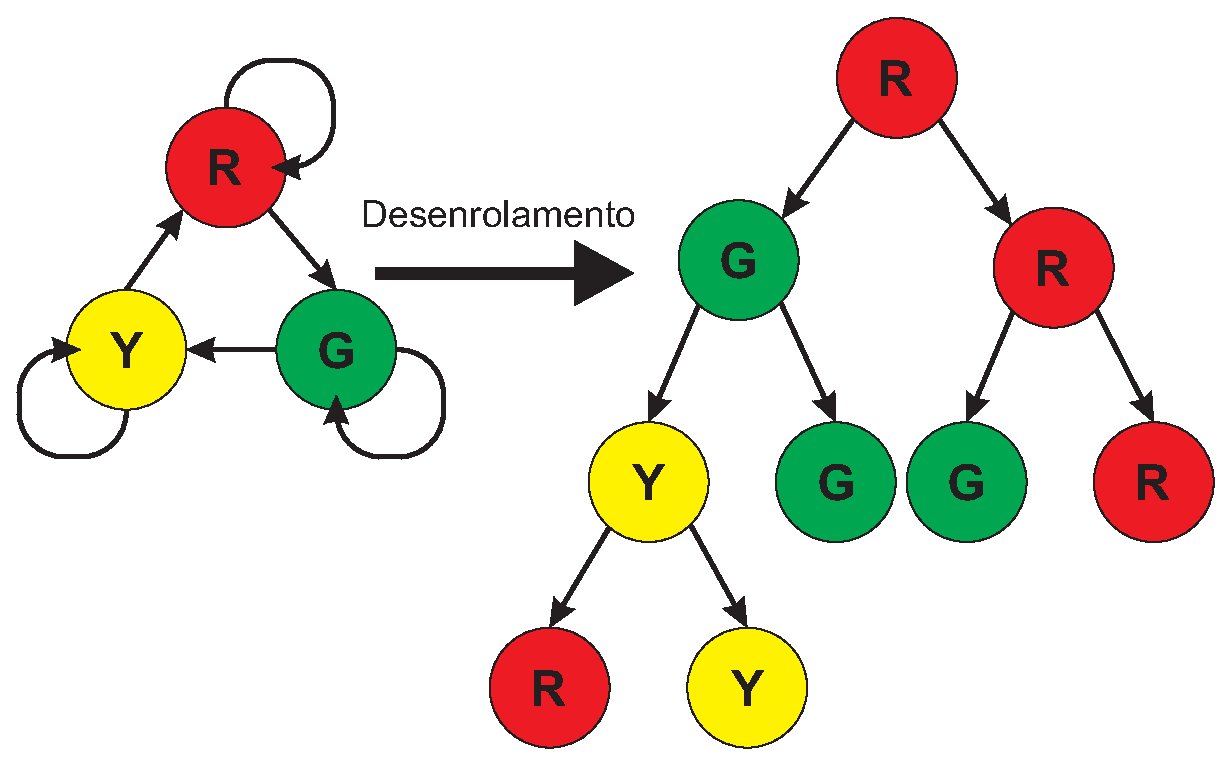
\includegraphics[scale=0.35]{figures/Tree}
  \caption{Desenrolamento do grafo de transi��o de estado.}
  \label{figure:tree}
\end{figure}

F�rmulas em CTL s�o constru�das a partir de proposi��es at�micas (onde cada proposi��o corresponde a uma vari�vel no modelo), conectivos booleanos padr�o de l�gica proposicional (por exemplo, e ($\lor$), ou ($\wedge$), ou-exclusivo($\veebar$), nega��o ($\lnot$)) e operadores temporais. Cada operador temporal consiste em duas partes: um quantificador de caminho (\textbf{A} ou \textbf{E}) seguido por uma modalidade temporal (\textbf{F}, \textbf{G}, \textbf{X}, \textbf{U}). Todos os operadores temporais s�o interpretados em rela��o a um estado atual impl�cito. Existem, em geral, muitos caminhos de execu��o (sequ�ncias de transi��es de estado) do sistema, come�ando no estado atual. O quantificador de caminho indica se a modalidade define uma propriedade que deve ser verdadeira para todos os caminhos poss�veis (denotada pelo quantificador de caminho universal \textbf{A}) ou se a propriedade precisa apenas de algum caminho (denotado pelo quantificador de caminho existencial \textbf{E}). As modalidades temporais descrevem a ordena��o de eventos no tempo ao longo de um caminho de execu��o e t�m o seguinte significado intuitivo:

\begin{enumerate}
\item $\textbf{F}\phi$ (l�-se ``$\phi$ vale no futuro'') � verdadeiro de um caminho se existir um estado no caminho onde a f�rmula $\phi$ � verdadeira;
\item $\textbf{G}\phi$ (l�-se ``$\phi$ vale globalmente'') � verdadeiro de um caminho se $\phi$ for verdadeiro em todos os estados no caminho;
\item $\textbf{X}\phi$ (l�-se ``$\phi$ vale no pr�ximo estado'') � verdadeiro de um caminho se $\phi$ � verdadeiro no estado alcan�ado imediatamente ap�s o estado atual no caminho;
\item $\phi\textbf{U}\psi$ (l�-se ``$\phi$ vale enquanto $\psi$ vale'', chamado ``forte at�'') � verdadeiro de um caminho se $\psi$ for verdadeiro em algum estado no caminho, e $\phi$ � v�lido em todos os estados anteriores.
\end{enumerate}

Cada f�rmula da l�gica � verdadeira ou falsa em um determinado estado; sua verdade � avaliada a partir da verdade de suas subf�rmulas de forma recursiva, at� chegar a proposi��es at�micas que s�o verdadeiras ou falsas em um dado estado. Uma f�rmula � satisfeita por um sistema se for verdadeira para todos os estados iniciais do sistema. Se a propriedade n�o for v�lida, o verificador de modelo produzir� um contraexemplo, que � um caminho de execu��o que testemunha a falha. Um algoritmo eficiente para verifica��o autom�tica de modelos foi descrito por Clarke \textit{et al.}~\cite{Clarke:1995}. A tabela a seguir mostra exemplos de avalia��es de f�rmulas na �rvore de computa��o da Figura~\ref{figure:tree}:

\begin{table}[htb]
	\renewcommand{\arraystretch}{1.0}
	\caption{Exemplos de avalia��es de f�rmulas na arvore de computa��o mostrada.}
	\label{table:ctl}
	\centering
	\begin{tabular}{c|c}
		\hline \bfseries F�rmula & \bfseries T/F\\
		\hline $\textbf{EG} (RED)$ & $True$\\
		\hline $\textbf{E} (RED \cup GREEN)$ & $True$\\
		\hline $\textbf{AF}(GREEN)$ & $False$\\
		\hline
	\end{tabular}
\end{table}

\subsubsection{Conten��o de Linguagem}\label{subsec:lc}

Existem propriedades de interesse pr�tico que n�o podem ser descritas no CTL. Um exemplo � a propriedade ``quase sempre'': uma condi��o, $\textbf{q}$, sempre se mant�m ap�s um n�mero finito de transi��es (note que as f�rmulas $\textbf{FG}$ $\textbf{q}$ e $\textbf{AFG}$ $\textbf{q}$ expressariam isso, mas estas n�o s�o f�rmulas legais de CTL). Esta propriedade se parece muito com $\textbf{AF}$ $\textbf{AG}$ $\textbf{q}$, mas n�o � o mesmo. Pode-se exibir um sistema de transi��o onde $\textbf{AF}$ $\textbf{G}$ $\textbf{q}$ � verdadeiro, enquanto $\textbf{AF}$ $\textbf{AG}$ $\textbf{q}$ � falso.
 
Uma solu��o seria usar um tipo mais expressivo de l�gica temporal (por exemplo, a propriedade anterior poderia ser expressa em Propositional Linear Temporal Logic (PLTL) ou CTL). Por�m haveria desvantagens, como a maior complexidade de algoritmos para verifica��o de modelos. Uma alternativa � usar outro paradigma de verifica��o, chamado conten��o de linguagem, baseado na teoria dos $\omega$-aut�matos. Por exemplo, � f�cil expressar a propriedade ``quase sempre'' anterior usando um aut�mato.

Para alcan�ar a verifica��o de conten��o de linguagem, representamos a composi��o do sistema dado com um modelo que representa a nega��o da propriedade e verificamos o vazio da linguagem. A linguagem do sistema composto est� vazia se e somente se o sistema satisfizer a propriedade $\textbf{T}$.
 
O vazio de linguagem � usado n�o apenas para verificar as propriedades que n�o podem ser expressas em \textit{Fair} CTL, mas tamb�m para verificar se a abstra��o de um sistema ainda cont�m o sistema original. Em ambos os casos, � preciso complementar um $\omega$-aut�mato ($\textbf{T}$), e isso � dif�cil de fazer se o aut�mato n�o for determin�stico (como � geralmente o caso de uma abstra��o). O fato de que a complementa��o de uma propriedade determinista � f�cil, enquanto a complementa��o de uma propriedade n�o-determin�stica pode ser dif�cil, � um problema-chave com a conten��o da linguagem. Isto levou a muita pesquisa em diferentes classes de $\omega$-aut�matos com diferentes expressividade e dificuldade de complementa��o.

\section{Sistemas Din�micos Lineares}\label{sec:lds}

\subsection{Cont�nuos}\label{subsec:c}

\subsection{Discretos}\label{subsec:d}

\subsection{Processo de Discretiza��o}\label{subsec:pd}

\subsection{An�lise Quantitativa da Resposta ao Degrau}\label{subsec:aqrd}

\section{T�cnicas de Projeto de Controle para Sistemas Discretos}\label{sec:tpcsd}

\subsection{Aloca��o de Polos}\label{subsec:ap}

\subsection{Regulador Quadr�tico Linear}\label{subsec:rql}

\subsection{S�ntese Indutiva Guidada por Contra Exemplos - CEGIS}\label{subsec:cegis}

\section{Implementa��o de Controladores Digitais}\label{subsec:icd}

\subsection{Efeitos de Palavra Finita}\label{subsec:fwl}



SMT (\textit{Satisfiability Modulo Theories}) verifica a satisfatibilidade de f�rmulas de primeira ordem a partir de uma ou mais teorias de fundamenta��o, que s�o compostas por um conjunto de senten�as. De modo formal, $\sigma$ -- \textit{theory} � uma cole��o de senten�as sobre a assinatura $\sigma$. Dada uma teoria $T$, diz-se que $\varphi$ � um m�dulo satisfat�vel de $T$ se $T \subset {\phi}$. Em outra defini��o, pode-se dizer que uma teoria $T$ � definida como uma classe de estruturas e $\varphi$ � um m�dulo satisfat�vel se existe uma estrutura $M$ em $T$ que satisfaz $\varphi$ (\textit{i.e.}, $M \models \varphi$)~\cite{Moura:2009}.

Solucionadores SMT como o Z3~\cite{Moura:2008} e Boolector~\cite{Brummayer:2009} suportam diferentes tipos de teorias, de modo que o seu desempenho pode variar conforme a sua implementa��o.

\begin{table}[htb]
	\renewcommand{\arraystretch}{1.0}
	\caption{Exemplos de teorias suportadas.}
	\label{table:smt}
	\centering
	\begin{tabular}{c|c}
		\hline \bfseries Teoria & \bfseries Exemplo\\
		\hline Igualdade & $x_1 = x_2 \wedge \neg (x_2 = x_3) \Rightarrow \neg (x_1 = x_3)$\\
		\hline Aritm�tica Linear & $(7y_1 + y_2 \geq 5) \vee (y_2 + y_3 \leq 2)$\\
		\hline Vetores de $bit$ & $(b \gg i) \& 1 = 1$\\
		\hline Arranjos & $store(a, j, 5) \Rightarrow a[j] = 5$\\
		\hline Teorias Combinadas & $(j \leq k \wedge a[j] = 2) \Rightarrow a[i] < 3$\\
		\hline
	\end{tabular}
\end{table}

A Tabela~\ref{table:smt} mostra algumas das teorias suportadas pelos solucionadores SMT utilizados neste trabalho. A teoria de igualdade permite verifica��es de igualdade e desigualdade entre predicados utilizando os operadores ($=$) ($\leq$) ($<$). A teoria da aritm�tica linear � respons�vel apenas pelas fun��es aritm�ticas (adi��o, subtra��o, multiplica��o e divis�o) entre vari�veis e constantes num�ricas. A teoria de vetores de $bit$ permite opera��es $bit$ a $bit$ considerando diferentes arquiteturas (\textit{e.g.}, $32$ e $64$ $bits$), nela est�o presentes os operadores: e ($\&$), ou ($\mid$), ou-exclusivo ($\bigoplus$), complemento ($\sim$), deslocamento para a direita ($\gg$) e deslocamento para a esquerda ($\ll$). Al�m disso, a teoria de arranjos permite a manipula��o de operadores como $select$ e $store$.

Em contraste com as f�rmulas geradas na satisfa��o booleana, que s�o apenas compostas por vari�veis booleanas, as quais podem assumir valores verdadeiro e falso e conectivos l�gicos, as f�rmulas de primeira ordem s�o formadas por conectivos l�gicos, vari�veis, quantificadores, fun��es e s�mbolos de predicado~\cite{Moura:2009}. De modo geral, as teorias do m�dulo da satisfatibilidade tem sido aplicadas em diversos cen�rios~\cite{Moura:2018}, apresentando resultados mais promissores (se comparados � satisfa��o booleana), incluindo o suporte a diferentes teorias de decis�o~\cite{Moura:2008, Moura:2009}.

\subsection{\textit{Efficient SMT-based Context-Bounded Model Checker}}\label{sec:esbmc}

O ESBMC � um verificador de modelos limitado ao contexto baseados nas teorias de m�dulo da satisfiabilidade (SMT), o qual � usado para verificar programas ANSI-C~\cite{Cordeiro:2012,DBLP:conf/tacas/MorseRCN014}. O ESBMC pode verificar tanto programas sequenciais quanto concorrentes e verifica propriedades relacionadas a estouro aritm�tico, divis�o por zero, acesso ilegal a posi��es em mem�ria, seguran�a de ponteiros, bloqueios fatais e corrida de dados. Esse processo � totalmente autom�tico e n�o requer intera��o de usu�rio para anotar programas com pr�- e/ou p�s-condi��es.

No ESBMC, o programa a ser verificado � modelado como um sistema de transi��o de estados $M = (S, R, s_0)$, 
que � extra�do de um gr�fico de fluxo de controle (GFC). $S$ representa o conjunto de estados, $R \subseteq S \times S$ representa o conjunto de transi��es ({\it i.e.}, pares de estados que especificam como o sistema pode navegar de um estado para outro) e $s_0 \subseteq S$ representa o conjunto de estadaos iniciais. Um estado $s \in S$ consiste de um valor do contador de programa $pc$ e os valores de todas as vari�veis do programa. Um estado inicial $s_0$ atribui a localiza��o inicial do programa do GFC para o $pc$. Cada transi��o $\gamma = (s_i, s_{i+1}) \in R$ entre dois estados $s_i$ and $s_{i+1}$ � identificada como uma f�rmula l�gica $\gamma (s_i,s_{i+1})$ que captura as restri��es nos valores do contador de programa e das vari�veis do programa correspondentes.

Dado um sistema de transi��o $M$, uma propriedade de seguran�a $\phi$, um limite de contexto $C$ e um limite $k$, o ESBMC constr�i uma �rvore de alcan�abilidade (AA) que representa o desdobramento do programa para $C$, $k$ e $\phi$. Ele ent�o deriva uma condi��o de verifica��o (CV)$\psi^{\pi}_k$, para cada intercala��o (ou caminho de computa��o) dada $\pi = \{v_1,...,v_k\}$, que � dada pela seguinte f�rmula l�gica:

\begin{equation}
\label{eq:bounded-model-checking}
    \psi^{\pi}_{k} =
    \overbrace{I(s_{0}) \wedge \bigvee_{i=0}^{k} \bigwedge_{j=0}^{i-1} \gamma(s_j,s_{j+1})}^{\textrm{restri��es}}
    \wedge \overbrace{\neg \phi(s_i)}^{\textrm{propriedade}}
\end{equation}

Aqui, $I$ caracteriza o conjunto de estados iniciais $M$ e $\gamma(s_j,s_{j+1})$ � a rela��o de $M$ entre passos de tempo $j$ e $j+1$. Consequentemente, $I(s_0) \wedge \bigvee_{j=0}^{i-1} \gamma (s_j,s_{j+1})$ representa a executa��o de $M$ de largura $i$ e $\psi^{\pi}_{k}$ pode ser satisfat�vel se e somente se para algum $i \leq k$ existe um estado alcan��vel ao longo de $\pi$ em um passo de tempo $i$ no qual $\phi$ � violada. $\psi^{\pi}_{k}$ � uma f�rmula livre de quantificadores em um subconjunto de l�gica de primeira ordem decid�vel, o qual sua satisfiabilidade � verificada por um solucionador SMT. Se $\psi^{\pi}_{k}$ � satisfat�vel, ent�o $\phi$ � violada ao longo de $\pi$ e o solucionador SMT fornece uma atribui��o satisfat�ria, da qual pode-se extrair valores para vari�veis do programa e construir um contraexemplo. Um contraexemplo para uma propriedade $\phi$ � uma sequ�ncia de estados $s_0,s_1,...,s_k$ com $s_0 \in S_0$, $s_k \in S$, e $\gamma (s_i, s_{i+1})$ para $0 \leq i < k$. Se $\psi^{\pi}_{k}$ n�o � satisfat�vel, pode-se concluir que nenhum estado de erro � alcan��vel em $k$ passos ou menos ao longo de $\pi$. Finalmente, pode-se definir $\psi_{k} = \bigwedge_{\pi} \psi_{k}^{\pi}$ e us�-la para verificar todos os caminhos.

No entanto, o ESBMC combina verifica��o de modelos simb�lica com a explora��o expl�cita do espa�o de estados; em particular, ele explicitamente explora todas as poss�veis intercala��es (at� o limite de contexto dado) enquanto ele trata cada intercala��o em si simbolicamente. O ESBMC implementa diferentes varia��es dessa abordagem, que diferem no modo que elas s�o exploradas na AA. A varia��o mais eficaz simplesmente percore a AA em profundidade e chama o procedimento BMC sequencial para cada intercala��o quando ela atinge um nodo folha da AA. Ele p�ra ou quando encontra erro ou sistematicamente explorou todas as poss�veis intercala��es da AA.

O modelo de mem�ria do ESBMC usa an�lise est�tica de ponteiros, preenchimentos em estruturas, com o objetivo de alinhar todos os campos aos limites de palavra, for�amento de regras de alinhamento de acesso de mem�ria e aloca��o de vetores de bytes, quando o tipo de aloca��o de mem�ria n�o � claro, para que a f�rmula SMT n�o seja t�o extensa e suscet�vel a erros.

O ESBMC tamb�m implementa a prova por indu��o~\cite{MorseCNF13,Gadelha:2017} para verificar propriedades em programas, \textit{i.e.}, utilizar uma abordagem iterativa de aprofundamento para checar se uma propriedade de seguran�a $\phi$ � satisfeita em cada passo $k$. O ESBMC usa um algoritmo \textit{k-induction}, que consiste de tr�s casos diferentes: caso base, condi��o adiante e passo indutivo. No caso base tenta-se encontrar um contraexemplo em at� $k$ desdobramentos de la�o; na condi��o adiante verifica-se se os la�os foram completamente desdobrados e que $\phi$ � v�lida em todos os estados alcan��veis dentro de $k$ passos; no passo indutivo assegura-se que sempre que $\phi$ � v�lida para $k$ desdobramentos, ela tamb�m � v�lida ap�s o pr�ximo desdobramento do sistema.

Uma outra aplica��o do ESBMC � a verifica��o de programas concorrentes para a plataforma CUDA~\cite{PereiraAMSCCSF16,Pereira:2016}. Utilizando um modelo operacional, \textit{i.e.}, uma representa��o abstrata das bibliotecas CUDA padr�es que aproxima de forma conservadora as suas sem�nticas, o ESBMC � capaz de verificar propriedades de seguran�a em programas CUDA. Al�m disso, o ESBMC implementa a redu��o parcial de ordem e a an�lise de duas \textit{threads} para minimizar a explora��o de espa�o de estados.

\section{Localiza��o de Falhas e Verifica��o de Modelos}\label{sec:fault-localization-and-model-checking}

\subsection{Uso de Contraexemplos para Localizar Falhas}\label{sec:using-counterexamples}

Em verifica��o de modelos, a atividade mais essencial, em rela��o � localiza��o de falhas, � a de gera��o de um contraexemplo, o qual � produzido quando um programa n�o satisfaz uma dada especifica��o. Um contraexemplo n�o prov� unicamente informa��es sobre a rela��o causa-efeito de uma dada viola��o, mas ele tamb�m pode auxiliar na localiza��o de falhas, como Clarke {\it et al.}~\cite{Clarke:2003,Clarke:1995} citam. Mas, visto que uma grande massa de informa��o � obtida em um contraexemplo, as linhas de fato defeituosas n�o s�o facilmente identificadas.

Alguns m�todos foram propostos, com o objetivo de localizar poss�veis causas de falha, usando contraexemplos. Ball {\it et al.}~\cite{Ball:2003} propuseram uma abordagem que tenta isolar poss�veis causas de contraexemplos, gerados pelo verificador de modelos SLAM~\cite{Ball:2001}. A ideia � que potenciais linhas defeituosas podem ser isoladas atrav�s de uma compara��o entre as transi��es obtidas em contraexemplos e execu��es bem-sucedidas, visto que transi��es n�o presentes em rastreamentos bem-sucedidos s�o potenciais causas de erros. Groce {\it et al.}~\cite{Groce:2003} afirmam que se um contraexemplo existe, um caminho similar mas n�o-defeituoso tamb�m existe e pode ser obtido usando t�cnicas de BMC. Elementos de programa relacionados a uma dada viola��o s�o sugeridos pelas diferen�as entre tal contraexemplo e um caminho bem-sucedido. Tal abordagem � implementada no verificador de modelos {\it Java PathFinder}~\cite{JPF} e tamb�m pode porver caminhos de execu��o que levam a estados err�neos, com rela��o a programasa concorrentes ({\it e.g.}, corrida de dados). O conceito chave da abordagem descrita por Groce {\it et al.}~\cite{Groce:2006} � similar ao anterior e usa alinhamento de restri��es para associar estados, em um contraexemplo, com os estados correspondentes em uma execu��o n�o-defeituosa, os quais s�o gerados por um solucionador de restri��es. Os estados mencionados s�o estados abstratos sobre predicados, os quais representam estados concretos em uma execu��o. Usando propriedades de m�tricas de dist�ncia, restri��es podem ser aplicadas para representar execu��es do programa, e restri��es sem correspondentes que representam estados concretos possivelmente levam a falhas. E ainda, se uma propriedade de m�tricas de dist�nica n�o � satisfeita, um contraexemplo � gerado pelo verificador de modelos~\cite{Groce:2006}.

\subsection{Localiza��o de Falhas em Programas Sequenciais}\label{sec:sequential-fault-localization}

Griesmayer {\it et al.}~\cite{Griesmayer:2007} propuseram um m�todo baseado em t�cnicas de BMC que pode diretamente identificar potenciais falhas em programas. Em particular, o m�todo usa vari�veis num�ricas adicionais, {\it e.g.} \texttt{diag}, para apontar linhas defeituosas em um dado programa.

Cada linha do programa, representando uma declara��o \texttt{S}, � transformada em uma vers�o l�gica de tal declara��o. Logo, o valor atribu�do a \texttt{S} � ou n�o-deterministicamente escolhido pelo verificador de modelos (se o valor de \texttt{diag} for o mesmo que o representado pela linha relacionada � declara��o \texttt{S}) ou o especificado originalmente. Os valores de \texttt{diag} obtidos pelo verificador de modelos representam linhas do programa e est�o estritamente ligados � falha obtida, visto que, corrigindo essa linha no programa original, a falha em quest�o pode ser evitada. No caso de m�ltiplos valores de \texttt{diag}, corrigindo tais linhas levam a uma execu��o bem sucedida do programa. Com o intuito de encontrar o conjunto inteiro de linhas que causam o comportamento defeituoso no programa, uma nova especifica��o no comando de verifica��o\footnote{\texttt{assume(diag != a)}} pode ser adicionada ao c�digo-fonte, o qual ent�o � executado novamente pelo verificador de modelos. Esse processo � executado repetidamente at� que n�o sejam obtidos novos valores para \texttt{diag}, {\it i.e.}, a execu��o n�o falha~\cite{Griesmayer:2007_2}.

Para ilustrar o funcionamento do m�todo em quest�o, toma-se como exemplo um controlador digital baseado na f�rmula da fun��o hor�ria do movimento retil�neo uniformemente variado (MRUV)~\cite{Ohanian:2006} (veja Equa��o~\ref{equation:space-equation}). A equa��o do controlador � definida na Equa��o~\ref{equation:controller-equation} (os valores foram atribu�dos arbritariamente).

\begin{gather}
  s(t) = at^2/2+v_0t+s_0 \label{equation:space-equation}
\end{gather}

\begin{gather}
  c(t) = t^2-3t+2 \label{equation:controller-equation}
\end{gather}

Um modelo na linguagem C do controlador � modelado como na Figura~\ref{figure:sequential-code}.

\begin{figure}[ht]
\centering
\begin{minipage}{0.65\textwidth}
\begin{lstlisting}
#include <stdio.h>
#include <assert.h>

const int A = 1;
const int B = -2;
const int C = 2;

int controller(int input) {
  int output = A * input * input + B * input + C;
  return output;
}

int main() {
  assert(controller(0) == 2 && controller(1) == 0 && controller(2) == 0 && controller(3) == 2);
  return 0;
}
\end{lstlisting}
\end{minipage}
\caption{C�digo sequencial de um controlador qualquer.}
\label{figure:sequential-code}
\end{figure}

Pode-se observar que o modelo n�o est� em conformidade com a equa��o dada, no caso o termo $B$ est� com o valor $-2$ ao inv�s de $-3$. Dessa forma, espera-se que a assertiva falhe ao executar o programa em um verificador de modelos, como pode ser observado no trecho da Figura~\ref{figure:counterexample-model} (o contraexemplo completo est� dispon�vel no Ap�ndice~\ref{appendix:counterexample-1}).

\begin{figure}[ht]
\centering
\begin{minipage}{0.65\textwidth}
\begin{lstlisting}
...
Violated property:
  file model.c line 14 function main
  assertion 
  FALSE

VERIFICATION FAILED
\end{lstlisting}
\end{minipage}
\caption{Trecho do contraexemplo para o modelo.}
\label{figure:counterexample-model}
\end{figure}

Usando o ESMBC como verificador de modelos, o c�digo instrumentado n�o-determin�stico obtido � como na Figura~\ref{figure:griesmayer-method-applied-code}.

\begin{figure}[ht]
\centering
\begin{minipage}{0.65\textwidth}
\begin{lstlisting}
#include <stdio.h>
#include <assert.h>
const int A = 1;
const int B = -2;
const int C = 2;
int nondet(int i) {
  int ret;
  __ESBMC_assume(ret != i);
  return ret;
}
int controller(int input) {
  int diag = nondet(0);
  int ta = (diag == 1 ? nondet(A) : A) * input * input;
  int tb = (diag == 2 ? nondet(B) : B) * input;
  int tc = (diag == 3 ? nondet(C) : C);
  int output = ta + tb + tc;
  return output;
}
int main() {
  __ESBMC_assume(controller(0) == 2 && controller(1) == 0 && controller(2) == 0 && controller(3) == 2);
  assert(0);
  return 0;
}
\end{lstlisting}
\end{minipage}
\caption{C�digo sequencial instrumentado com o m�todo descrito aplicado.}
\label{figure:griesmayer-method-applied-code}
\end{figure}

Ao executar o c�digo da Figura~\ref{figure:griesmayer-method-applied-code} no ESBMC sucessivamente, \textit{i.e.}, at� que n�o sejam encontrados novos valores para $diag$, obt�m-se os valores presentes na Figura~\ref{figure:faulty-lines-griesmayer} (o contraexemplo completo est� dispon�vel no Ap�ndice~\ref{appendix:counterexample-2}).

\begin{figure}[ht]
\centering
\begin{minipage}{0.65\textwidth}
\begin{lstlisting}
griesmayer::controller::1::diag=-2012462479 (-2012462479)
griesmayer::controller::1::diag=2 (2)
griesmayer::controller::1::diag=2 (2)
griesmayer::controller::1::diag=2 (2)
\end{lstlisting}
\end{minipage}
\caption{Linhas defeituosas obtidas pela execu��o do c�digo~\ref{figure:griesmayer-method-applied-code}.}
\label{figure:faulty-lines-griesmayer}
\end{figure}

Segundo o contraexemplo obtido com o ESBMC, pode-se observar que o valor de $diag$ � $2$ em tr�s casos e um inteiro negativo em um caso. Logo, o problema est� no c�lculo do segundo termo, como esperado. O contraexemplo completo mostra que o valor para corrigir tal falha � $-3$. Assim, pode-se corrigir a falha apontada e reexecutar o c�digo no verificador de modelos.

\begin{figure}[ht]
\centering
\begin{minipage}{0.65\textwidth}
\begin{lstlisting}
#include <stdio.h>
#include <assert.h>
const int A = 1;
const int B = -3;
const int C = 2;
int controller(int input) {
  int output = A * input * input + B * input + C;
  return output;
}
int main() {
  assert(controller(0) == 2 && controller(1) == 0 && controller(2) == 0 && controller(3) == 2);
  return 0;
}
\end{lstlisting}
\end{minipage}
\caption{C�digo sequencial corrigido.}
\label{figure:corrected-sequential-code}
\end{figure}

Ap�s a corre��o do problema apontado, executa-se o c�digo corrigido~\ref{figure:corrected-sequential-code} no ESBMC e obt�m-se as linhas presentes na Figura~\ref{figure:correct-faulty-lines-griesmayer} (o contraexemplo completo est� dispon�vel no Ap�ndice~\ref{appendix:counterexample-3}). Em controladores digitais, � importante que os modelos sejam precisamente especificados para evitar falhas durante o funcionamento em ambiente real, visto que podem levar ao mal-funcionamento do equipamento e at� danos, aumentando o custo do mesmo.

\begin{figure}[ht]
\centering
\begin{minipage}{0.65\textwidth}
\begin{lstlisting}
griesmayer::controller::1::diag=-934770697 (-934770697)
griesmayer::controller::1::diag=-1 (-1)
griesmayer::controller::1::diag=-1 (-1)
griesmayer::controller::1::diag=-1 (-1)
\end{lstlisting}
\end{minipage}
\caption{Linhas defeituosas obtidas pela execu��o do c�digo~\ref{figure:corrected-sequential-code}.}
\label{figure:correct-faulty-lines-griesmayer}
\end{figure}

Dessa forma, foi poss�vel observar o m�todo proposto por Griesmayer {\it et al.}~\cite{Griesmayer:2007} aplicado em um programa sequencial.

Este m�todo foi escolhido para ser utilizado neste trabalho, pois al�m de ser simples a sua implementa��o, ele aponta n�o s� linhas que cont�m defeitos, como tamb�m poss�veis valores que levam a uma execu��o bem-sucedida do programa original.

\section{Resumo}\label{sec:chap-2-summary}

Neste cap�tulo, foram introduzidos os conceitos b�sicos para o entendimento desta disserta��o, relacionadas � verifica��o de modelos. Mais especificamente, explicou-se o conceito de verifica��o de modelos limitada usando teorias de m�dulo da satisfiabilidade (SMT) com o verificador de modelos ESBMC ({\it Efficient SMT-based Context-Bounded Model Checker}), que verifica propriedades de programas sequenciais e concorrentes. Tamb�m foram mostradas discuss�es sobre o uso de contraexemplos para auxiliar no processo de localiza��o de falhas. Por fim, foi apresentado um m�todo para localizar falhas em programas sequenciais, usando n�o-determinismo para instrumentar atribui��es, de forma que o verificador de modelos escolhe o valor para cada vari�vel do programa para que propriedade (em forma de assertiva) presente no c�digo seja satisfeita. Como resultado, o cont�udo deste cap�tulo fornece todo o embasamento necess�rio para compreens�o do trabalho desenvolvido, que ser� descrito nas se��es subsequentes.

\chapter{Trabalhos Relacionados}\label{chap_related_work}

Neste cap�tulo, ser�o descritos oito trabalhos relacionados que direta ou indiretamente abordam localiza��o de falhas em programas concorrentes. Apesar de existirem outros estudos relacionados ao tema, foram selecionados apenas os que se assemelham a este trabalho.

Cada trabalho relacionado ser� descrito de acordo com suas caracter�sticas mais relevantes. Ao final de cada subse��o ser�o destacados os melhores aspectos e os pontos fracos de cada um. Por fim, ser� feito um paralelo das caracter�sticas que s�o importantes para os objetivos propostos neste trabalho, que servir� como base de compara��o.

\section{\textit{Formal Non-Fragile Stability Verification of Digital Control Systems with Uncertainty}}\label{sec:related-work-1}

Bessa {\it et al.}~\cite{bessa2017formal} apresentam uma metodologia de verifica��o para determinar formalmente a estabilidade incerta de sistemas lineares em controladores digitais com considera��es sobre os aspectos de implementa��o. Especificamente, esta estrat�gia � combinada com o DSVerifier, que � uma ferramenta de verifica��o que utiliza a verifica��o de modelo limitado com base nas teorias de m�dulo de confiabilidade (SMT) para verificar a estabilidade dos sistemas de controle digital considerando incerteza. O DSVerifier determina a estabilidade do sistema de controle, considerando a planta, juntamente com os efeitos do comprimento da palavra finita (FWL) na implementa��o do controlador digital. Em seguinda, verifica-se a estabilidade robusta ``n�o fr�gil'' de um determinado sistema em malha fechada. A metodologia proposta e a respectiva ferramenta (DSVerifier) s�o avaliadas considerando exemplos de controle n�o fr�geis encontrados na literatura.

O trabalho mostra que a t�cnica � capaz de prever problemas de fragilidade em controladores robustos quando consideramos a estabilidades de sistemas de controle digital, visto que leva em considera��o os efeito FWL. No entanto, este trabalho se prende a apenas verificar a estabilidade, sendo que aspectos de desempenho s�o deixados de lado, visto que as propriedades de desempenho s�o super importantes quando se projeta controladores, al�m de j� considerarem a estabilidade.

\section{\textit{Formal Analysis of Robustness at Model and Code Level }}\label{sec:related-work-2}

Wang {\it et al.}~\cite{WangGRJF16} apresentam uma abordagem de verifica��o da robustez de sistemas de controle, a nivel de c�digo e modelagem, onde se baseia em um c�lculo invariante na din�mica discreta do sistema. Usando solucionadores de programa��o semi-definida (SDP), uma fun��o baseada em Lyapunov � sintetizada, capturando as margens do vetor do sistema linear em malha fechada considerado. Essa invariante num�rica expressa sobre as vari�veis de estado do sistema � compat�vel com a an�lise de c�digo e permite sua valida��o no artefato de c�digo. Esta an�lise autom�tica amplia as t�cnicas de verifica��o focadas na implementa��o do controlador, abordando a valida��o da robustez no modelo e no n�vel de c�digo. Ele foi implementado em uma ferramenta que analisa sistemas SISO discretos e gera super-aproxima��es de margens de fase e ganho.

Os autores apresentam uma abordagem eficaz para verificar robustez dos controladores digitais a nivel de c�digo e modelagem. Novamente, esse trabalho emprega a verifica��o usando uma abordagem a nivel de c�digo, por�m n�o considera aspectos de desempenho do controlador, apesar de considerar aspectos relativos a efeitos causados pela aritm�tica de ponto fixo.

\section{\textit{Temporal Logic Control of Discrete-Time Piecewise Affine Systems}}\label{sec:related-work-3}

Yordanov {\it et al.}~\cite{yordanov2012temporal} apresentam uma estrutura computacional para s�ntese autom�tica de uma estrat�gia de controle de realimenta��o para um sistema de tempo discreto (mais precisamente sistemas PWA) a partir de uma especifica��o dada como uma l�gica linear temporal (LTL) sobre um conjunto arbitr�rio de predicados lineares nas vari�veis de estado do sistema. A abordagem consiste em definir parti��es apropriadas para seu estado e espa�os de entrada, e ent�o constr�i-se uma abstra��o finita do sistema na forma de um sistema de transi��o de controle. Depois disso, aproveitando ideias e t�cnicas de verifica��o de modelos LTL e jogos de Rabin, desenvelvoram um algoritmo para gerar uma estrat�gia de controle para a abstra��o finita.

A abordagem apresentada para a constru��o da abstra��o garante que uma estrat�gia de controle gerada para o sistema de controle finito pode ser facilmente transformada em uma estrat�gia de controle para o sistema PWA inicial. Embora comprovadamente correta, a solu��o geral � conservadora e computacionalmente cara. Apesar de esta abordagem conseguir sintetizar controladores, deixa de considerar alguns aspectos bem relevantes em projetos de controladores digitais, como aspectos de desempenho e efeitos da fragilidade de controladores quando implementados em microprocessadores.

\section{\textit{Formal Methods for Adaptive Control of Dynamical Systems}}\label{sec:related-work-4}

Sadraddini and Belta~\cite{sadraddini2017formal} desenvolveram um m�todo para controlar sistemas de tempo discreto com par�metros constantes mas inicialmente desconhecidos a partir de especifica��es de l�gica temporal linear (LTL).Os autores usam as no��es de sistemas de transi��o param�tricos e adaptativos (n�o-determin�sticos) e ferramentas de m�todos formais para computar estrat�gias de controle adaptativo para sistemas finitos. 

Apesar de n�o utilizar os m�todos tradicionais de controle adaptativo, usando uma abordagem correta por constru��o a qual n�o requer um modelo de refer�ncia e pode lidar com uma gama muito maior de sistemas e especifica��es, n�o leva em considera��o aspectos relativos a depensempenho de sistemas considerando a resposta ao degrau, bem como deixa de lado aspectos enfrentados com a implementa��o, como os efeitos de FWL. Como a maioria das outras aplica��es de m�todos formais, os resultados sofrem pela alta complexidade computacional. Como discutido no artigo, o n�mero de estados no sistema de transi��o adaptativa (ATS) pode ser muito grande. Al�m disso, a constru��o de quocientes finitos para sistemas infinitos � computacionalmente dif�cil.

\section{\textit{Correct-by-construction Adaptive Cruise Control: Two Approaches}}\label{sec:related-work-5}

Nilsosn {\it et al.}~\cite{nilsson2016correct} descrevem duas abordagens para sintetizar controladores correto por constru��o em sistemas de controle de cruzeiro adaptativo. Ambas as abordagens baseiam-se na computa��o em pontos fixos no dom�nio do controlador, a partir da qual a especifica��o em l�gica linear temporal (LTL) pode ser aplicada. Uma calcula tais pontos fixos diretamente no espa�o de estados cont�nuo, a outra em uma abstra��o de estados finitos da din�mica n�o-linear.

De acordo com os resultados experimentais, este trabalho se mostra eficaz para sistemas de controle de cruzeiro adaptativo. Por�m, leva em considera��o a s�ntese de controladores est�veis considerando a propriedade de \textit{safety}, mas n'ao aborda quest�es de projeto de controladores referentes a desempenho a resposta ao degrau.

\section{\textit{Formal Specification and Analysis Approaches for Spacecraft Attitude Control Requirements}}\label{sec:related-work-6}

Gross {\it et al.}~\cite{gross2017formal} propuseram uma abordagem para formalizar requisitos comuns de sistema de controle de atitude de naves espaciais, como limites do atuador, erro de indica��o, alcan�abilidade, desvio, tempo de assentamento, tempo de subida e sobressinal. Os autores utlizaram m�todos formais, mais especificamente verifica��o de modelos e teste de hip�tese para verificar requisitos de desempenho de sistemas de controle de atitude de naves espaciais. O trabalho em quest�o avalia esses sistemas e verifica se obedecem a esses requisitos no dom�nio do tempo cont�nuo. Embora a inten��o inicial de formalizar os requisitos fosse conduzir an�lises formais de m�todos para determinar se o projeto de controle de atitude de naves espaciais atendia aos requisitos do sistema, as equa��es de movimentos n�o-lineares se mostraram muito complexas para os solucionadores e apenas alguns requisitos puderam ser analisados.

Um ponto positivo desse trabalho foi que consideraram aspectos de desempenho na verifica��o de controladores. Apesar disso, os autores n�o trabalharam com sistemas em tempo discreto, n�o levando em considera��o aspectos de implementa��o, como os efeitos FWL.

\section{\textit{Robust Controller Synthesis of Switched Systems Using Counterexample Guided Framework}}\label{sec:related-work-7}

Ravanbakhsh and Sankaranarayanan~\cite{ravanbakhsh2016robust} investigam o problema de sintetizar controladores robustos que asseguram que o sistema em malha fechada satisfa�a uma especifica��o de \textit{reach-while-stay} de entrada, em que todas as trajet�rias partindo de um conjunto inicial $I$, eventualmente atingem um conjunto de metas especificadas $G$, enquanto permanecem dentro de um conjunto seguro $S$. A ideia chave �: dado o modelo da planta que consiste em um sistema comutado de tempo cont�nuo controlado por um sinal de comuta��o externo e entradas de perturba��o da planta, o controlador usa uma lei de realimenta��o de estado para controlar o sinal de comuta��o, a fim de garantir que as propriedades de corre��o desejadas sejam mantidas, independentemente das a��es de perturba��o. Para garantir a especifica��o de \textit{reach-while-stay}, a abordagem usa um certificado de prova na forma de uma fun��o robusta de controle Lyapunov (\textit{robust control Lyapunov-like function} - RCLF). Para encontrar um RCLF, usa-se uma estrutura de s�ntese indutiva guiada por contra-exemplo (CEGIS), resolvendo iterativamente uma f�rmula $\exists \forall \exists \forall$ usando solucionadores SMT livres de quantifica��o. Finalmente, utilizaram o problema de traduzir o RCLF sintetizado pela abordagem em uma implementa��o de controle.

A t�cnica de s�ntese de controladores para sistemas de controle comutados apresentada aparesentou bons resultados pelo que se propos a fazer, considerando sistemas de controle em tempo cont�nuo. Por�m, deixou de considerar aspectos de implementa��o desses controladores do mundo real, onde necessita-se trabalhar com sistemas em tempo discreto, e levar em conta aspectos de implementa��o, como efeitos de FWL. O problema de sintetizar controladores para satisfazer requisitos da propriedade \textit{reach-while-stay} tem sua import�ncia, mas outros aspectos como estabilidade e requisitos de desempenham devem ser considerados em projeto de controladores para problemas do mundo real.

\section{\textit{Multi-objective design of state feedback controllers using reinforced quantum-behaved particle swarm optimization}}\label{sec:related-work-8}

Hassani and Lee~\cite{hassani2016multi} apresentam um paradigma de projeto gen�rico multi-objetivo que utiliza otimiza��o de enxame de particulas (\textit{particle swarm optimization} - PSO) com comportamento qu�ntico (QPSO) para decidir a configura��o ideal do controlador LQR para um determinado problema, considerando um conjunto de objetivos concorrentes. Existem tr�s contribui��es principais introduzidas nesse trabalho da seguinte forma: o algoritmo QPSO padr�o � refor�ado com um esquema de inicializa��o informado baseado no algoritmo de recozimento simulado e no mecanismo de sele��o de vizinhan�a gaussiana, ele tamb�m � aumentado com uma estrat�gia de busca local que integra as vantagens do algoritmo mem�tico no QPSO convencional, e tamb�m � introduzido um crit�rio agregado de pondera��o din�mica que combina dinamicamente as restri��es \textit{soft} e \textit{hard} com os objetivos de controle para fornecer ao projetista um conjunto de solu��es �timas de Pareto e permite que ela decida a solu��o de destino com base nas prefer�ncias pr�ticas.

O trabalho em quest�o se mostra bastante promissor, visto que faz uma certa an�lise a aspectos de desempenho de sistemas de controle. Apesar disso, a an�lise toda � feita considerando controladores em tempo cont�nuo. Apenas � feito uma ``melhoria`` nos par�metros de desempenho do sistemas, mas n�o sintetiza controladores com base nesses par�metros como requisitos necess�rios e espec�ficos. Como n�o trabalha diretamente com sistemas de controle digital, consequentemente n�o leva em conta aspectos de implementa��o dos mesmo em microprocessadores, podendo gerar controladores que quando implementados nessas plataformas n�o se comporte conforme projetado, visto que podem sofrer com os efeitos de FWL, por exemplo.


\section{\textit{Formal Synthesis of Analytic Controllers for Sampled-Data Systems via Genetic Programming}}\label{sec:related-work-9}

Verdier {\it et al.}~\cite{verdier2018formal} apresentam um m�todo autom�tico de s�ntese de controladores para sistemas de amostragem de dados n�o-lineares com especifica��es de seguran�a e alcan�abilidade. Basicamente, a estrat�gia apresentada n�o se limita aos sistemas polinomiais e controladores. Considera-se ocasionalmente controladores comutados baseados em fun��es de barreira de controle Lyapunov. A estrat�gia proposta utiliza programa��o gen�tica para sintetizar essas fun��es, bem como os modos do controlador. A exatid�o do controlador � verificada por meio de um solucionador de hip�tese de m�dulo de satisfiabilidade.

De acordo com o estudo apresentado, a metodologia utlizada apresentou bons resultados, considerando o que os autores se propuseram a fazer. Apesar disso, testaram apenas em sistemas at� terceira ordem. Al�m do mais, trabalharam apenas com sistemas cont�nuos considerando somente estabilidade do sistemas e desconsiderando aspectos de implementa��o em sistemas microprocessados, como os efeitos de FWL.


\section{\textit{Automated Formal Synthesis of Digital Controllers for State-Space Physical Plants}}\label{sec:related-work-10}

Abate {\it et al.}~\cite{abate2017automated} prop�em uma abordagem s�lida e automatizada para sintetizar controladores digitais com realimenta��o seguros para plantas f�sicas representadas como modelos lineares invariantes no tempo. Os autores utilizaram s�ntese indutiva guiada por contra-exemplo (CEGIS) o qual possui duas fases: s�ntese de um controlador de realimenta��o est�tico que estabiliza o sistema, mas que pode n�o ser seguro para todas as condi��es iniciais. A seguran�a � ent�o verificada via verifica��o de modelos limitada (\textit{bounded model checking} - BMC) ou acelera��o abstrata; se a etapa de verifica��o falhar, um contra-exemplo � fornecido ao mecanismo de s�ntese e o processo itera at� que um controlador seguro seja obtido.

O trabalho em quest�o apresenta excelentes resultados, por�m ainda deixa de considerar aspectos de desempenho de projeto de controladores, considerando somente a estabilidade dos mesmos. Um bom aspecto � que a metodologia considera fragilidade na implementa��o dos controladores digitais.


\section{Compara��o entre os Trabalhos}

Os trabalhos relacionados tratam de verifica��o de sistemas de controle que � uma das fases deste trabalho, e s�ntese de controladores de sistemas de controle. Pode-se notar a respeito dos trabalhos analisados que o problema de s�ntese de controladores digitais � pertinente, visto que este processo � bastante necess�rio na fase de projeto de um controlador digital. A s�ntese de controladores digitais para sistemas de controle foi observado como um problema complexo e de dif�cil uma grande abrang�nciade problemas devido a muitos trabalhos abordarem o problema de diferentes maneiras e levando em considera��o fatores diferentes. Sabendo disso, as principais diferen�as entre a abordagem proposta nesse trabalho para as aqui discutidas podem ser listadas: trabalha com sistemas de controle em tempo discreto o qual � o que efetivamente � usado quando implementamos utilizando uma plataforma microprocesada; a metodologia proposta sintetiza e verifica controladores considerando requisitos de desempenho de sistemas de controle; e, finalmente, consideramos aspectos de implementa��o que podemn ocasionar mal funcionamento dos sistemas de controle, visto que os efeitos de FWL, por exemplo, podem levar a isso. A Tabela~\ref{table:related-work-comparison} mostra um quadro comparativo entre a metodologia proposto nesta disserta��o e os trabalhos relacionados selecionados.

\begin{table}[ht]
    \renewcommand{\arraystretch}{1.0}
    \caption{Compara��o dos trabalhos relacionados}
    \label{table:related-work-comparison}
    \centering
    \begin{tabular}{c|c|c|c|c}
        \hline \shortstack{\bfseries Trabalhos} & \bfseries Suporte a & \bfseries Suporte a & \bfseries Considera os & \bfseries S�ntese e\\
\bfseries relacionados & \bfseries sistemas & \bfseries requisitos de & \bfseries efeitos & \bfseries de casos\\
\bfseries & \bfseries discretos & \bfseries desempenho & \bfseries de FWL & \bfseries Verifica��o\\
        \hline Bessa {\it et al.} (2017) & X & & X & \\
        \hline Wang {\it et al.} (2016) & X & & & \\
        \hline Yordanov {\it et al.} (2012) & X & & & \\
        \hline Sadraddini and Belta (2017) & X & & & \\
        \hline Nilsosn {\it et al.} (2016) & X & & X & \\
        \hline Gross {\it et al.} (2017) & & X & & \\
        \hline Ravanbakhsh and Sankaranarayanan (2016) & & & & X\\
        \hline Hassani and Lee (2016) & & X & & \\
        \hline Verdier {\it et al.} (2018) & & & & \\
        \hline Abate {\it et al.} (2017) & X & & X & X\\
        \hline Metodologia proposta & X & X & X & X\\
	\end{tabular}
\end{table}

Atrav�s da Tabela~\ref{table:related-work-comparison} pode-se observar que existem outros trabalhos que s�o capazes de localizar falhas em programas concorrentes. No entanto, nenhum deles � capaz de atingir ambos objetivos em programas escritos na linguagem C e, ainda mais, sem o aux�lio de casos de teste previamente escritos, diferentemente do m�todo proposto.

\section{Resumo}\label{chap-3-summary}

Neste cap�tulo foram apresentados diversos trabalhos relacionados a algum dos seguintes problemas: localiza��o de falhas, suporte a programas concorrentes, verifica��o de c�digo escrito na linguagem C e/ou depend�ncia de casos de testes externos. Ap�s a apresenta��o de cada t�cnica, assim como uma breve discuss�o sobre as vantagens e desvantagens de cada uma delas, foi feita uma compara��o com o m�todo proposto neste trabalho. Foi poss�vel observar que o m�todo proposto aborda os tr�s primeiros itens sem a necessidade de casos de testes externos, o que o diferencia dos demais trabalhos. O pr�ximo cap�tulo apresenta a metodologia proposta para localizar falhas em programas concorrentes utilizando t�cnicas de sequencializa��o e BMC.
\chapter{A Metodologia Proposta}\label{chap_methodology}

Neste cap�tulo, a metodologia proposta para sintetizar controlodores digitais com realimenta��o de estados, considerando fragilidade e especifica��es de desempenho ser� completamente descrita. Primeiramente, mostraremos as metodologias formalizadas para verificar sistemas de controle digital, com respeito a especifica��es de performance, no caso m�ximo tempo de assentamento e m�ximo sobressinal. A formaliza��o utilizada para estimar o m�ximo sobressinal, bem como a invariante formalizada para verificar o m�ximo tempo de assentamento. Tamb�m s�o descritos os algoritmos criados para fazer a devida verifica��o das mesmas. Finalmente, a descri��o completa da t�cnica que utilizamos para realizar o processo de s�ntese.

\section{Vis�o Geral do M�todo}
\label{sec:method-overview}

Aqui, o m�todo proposto � descrito brevemente, como mostrado na Figura~\ref{figure:methodology}, e uma explica��o mais detalhada � exposta nas se��es seguitnes. Dado um programa concorrente $P$, primeiramente checa-se se ele apresenta uma execu��o mal-sucedida com rela��o a uma determinada intercala��o. Para realizar tal tarefa, $P$ � executado em um verificador de modelos duas vezes: a primeira execu��o verifica se existe algum bloqueio fatal e a segunda � respons�vel por outros tipos de viola��o, tais como erros de aquisi��o de sem�foro, divis�o por zero, seguran�a de ponteiros, estouro aritm�tico e viola��o de limites de vetores. N�o � poss�vel verific�-lo apenas uma vez porque os verificadores de modelos separam essas verifica��es, \textit{i.e.}, � necess�rio adicionar uma op��o de linha de comando para habilitar a detec��o de bloqueios fatais e ignorar viola��es devido a assertivas. Caso um contraexemplo possa ser obtido nesse passo, � poss�vel prosseguir com o m�todo. Ent�o, o pr�ximo passo define as regras de transforma��o, que s�o as instru��es sequenciais que substituir�o as originais concorrentes, e um arcabou�o sequencial, o qual tem como objetivo simular a execu��o concorrente da intercala��o mal-sucedida. O terceiro passo consiste em usar o m�todo proposto por Griesmayer~\cite{Griesmayer:2007} para instrumentar atribui��es e express�es, de forma a apontar locais e instru��es defeituosas do programa. Tal programa instrumentado pode ent�o ser executado, usando um verificador de modelos, e � poss�vel coletar as linhas defeituosas, at� que a verifica��o associada n�o produza diferentes elementos. Essa itera��o � descrita na Figura~\ref{figure:methodology} por meio dos passos $3$, $4$, j� que o m�todo busca novos contraexemplos, com o intuito de encontrar novas linhas defeituosas. Finalmente, as linhas defeituosas s�o obtidas, assim como atribui��es necess�rias para produzir uma execu��o bem-sucedida de $P$.

\begin{figure}[ht]
  \centering
  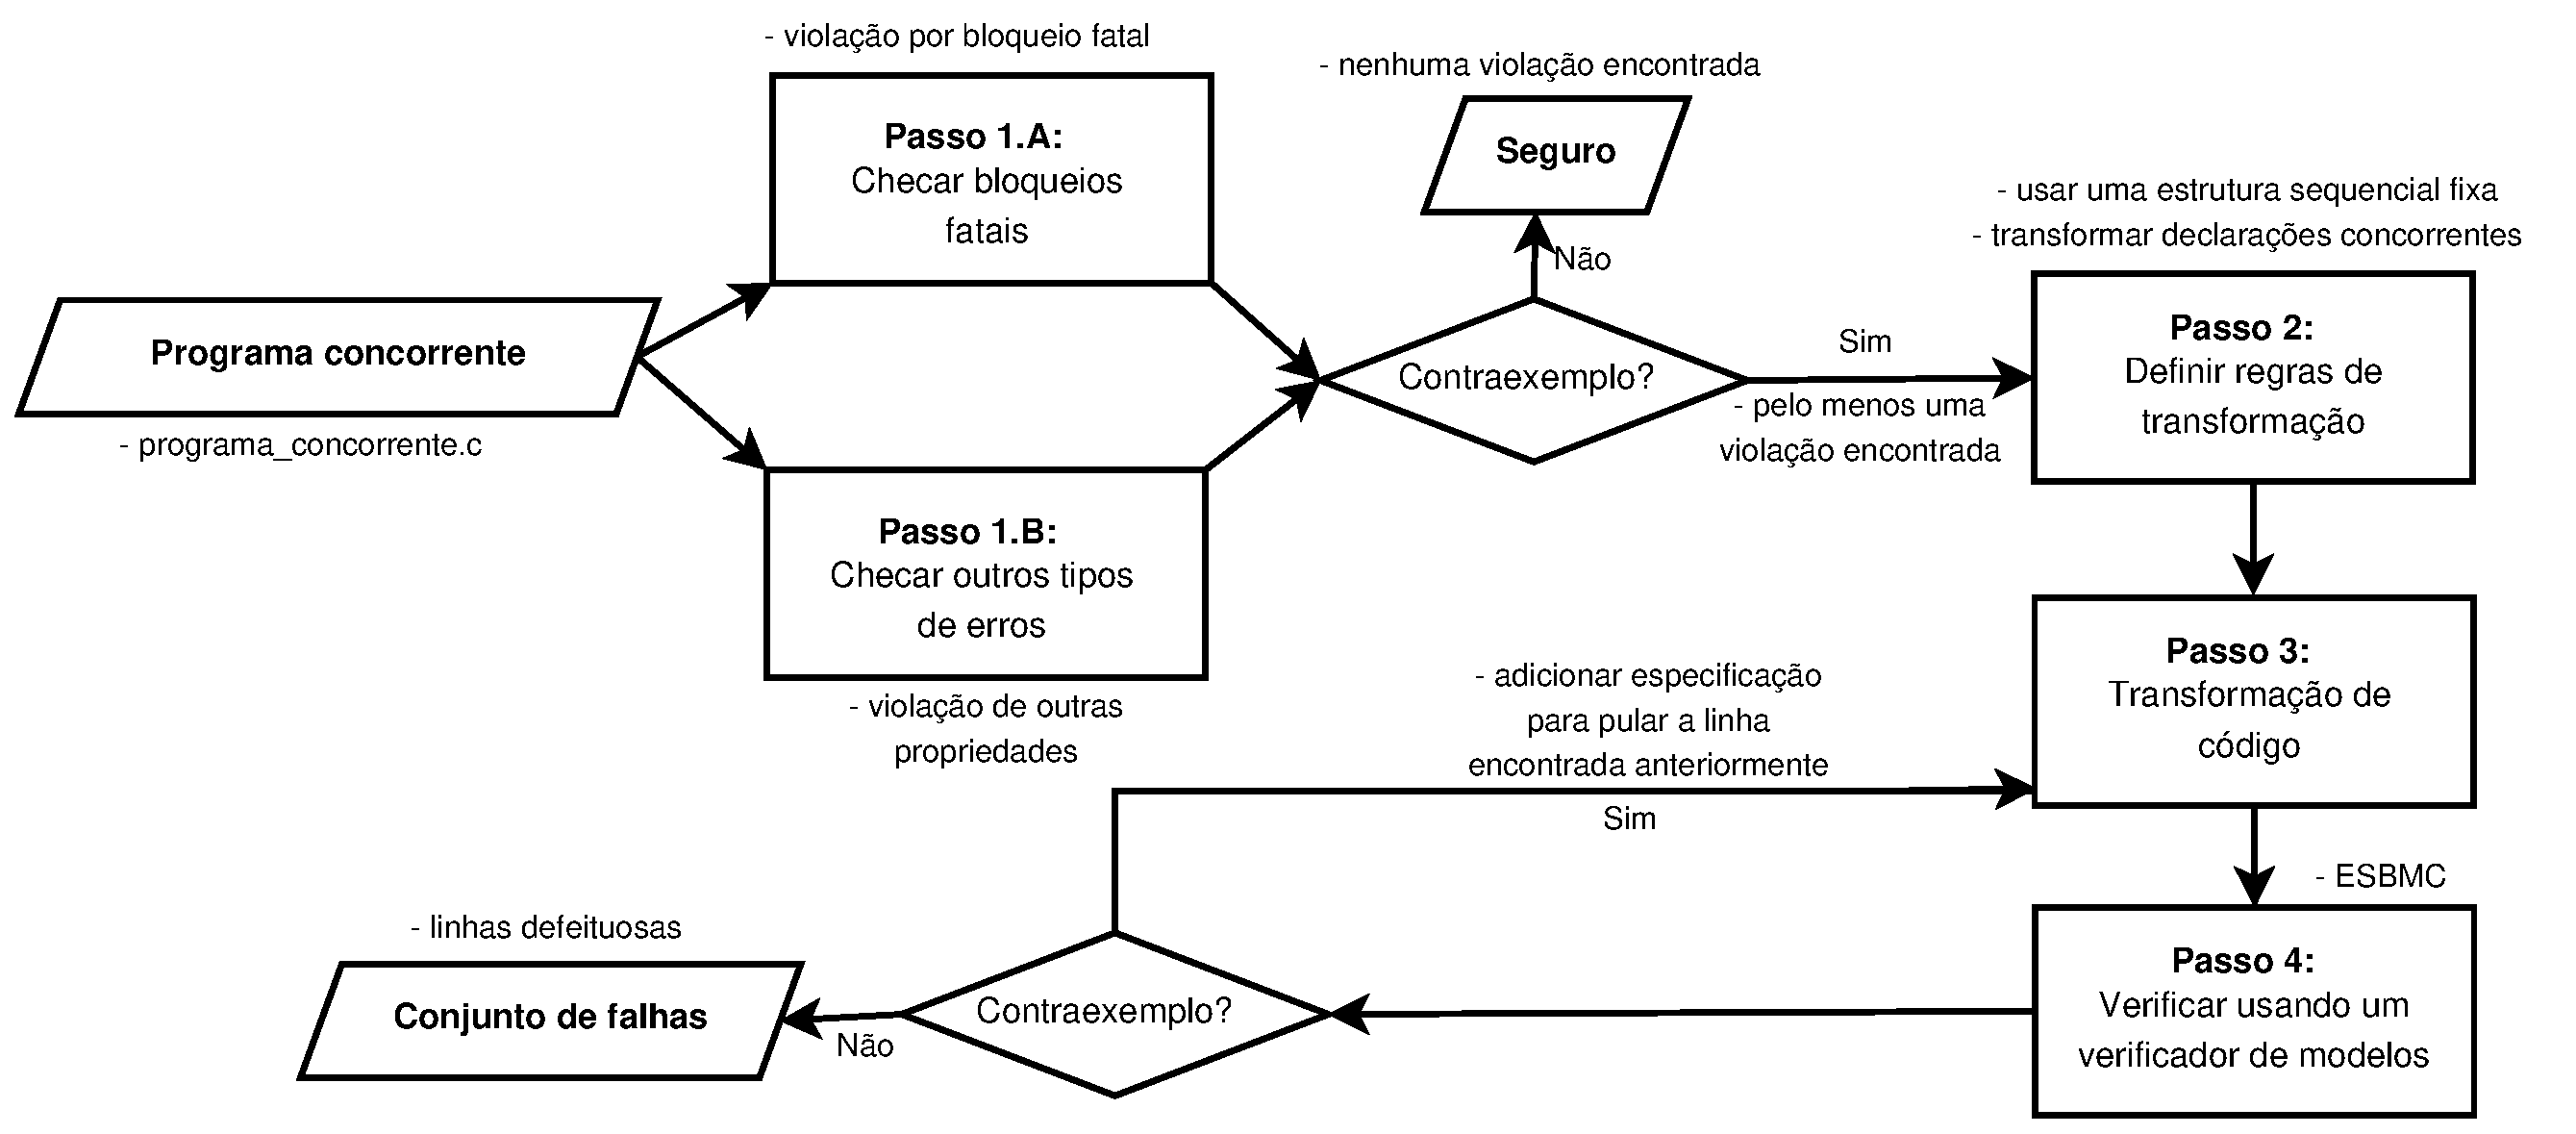
\includegraphics[scale=0.35]{figures/methodology}
  \caption{Metodologia proposta.}
  \label{figure:methodology}
\end{figure}

%-------------------------------------------------------------------
\section{Verifying Non-fragile Performance Specification Requirements}
\label{sec:verification}
%-------------------------------------------------------------------

As we described, in this work we use a variation of CEGIS synthesis to synthesize a controller in order to satisfy performance requirements in digital control systems such as settling-time and maximum overshoot. In CEGIS strategy of we have basically two main stages: synthesis and verification. In this section we show the verification method of settling-time and maximum overshoot of digital control systems.
%--------------------------------------------------------------------------------
\subsection{Maximum Overshooting Estimation}
\label{sec:modformver}
%--------------------------------------------------------------------------------

Algorithm~\ref{alg:overshootEst} describes a procedure for estimating $y_{\mathrm{p}}$ (maximum peak value in a system's response) and $k_{\mathrm{p}}$ (sample where $y_{\mathrm{p}}$ is located), in order to find a formal approach to verify the maximum overshoot used in our CEGIS approach.

%\begin{algorithm}
%    \caption{Estimation of $y_{\mathrm{p}}$ and $k_{\mathrm{p}}$}
%    \label{alg:overshootEst}
%    \begin{algorithmic}[1] % The number tells where the line numbering should start
%        \Procedure{estimate\_maxPeak\_value}{$   $}
%          \State $y_\mathrm{p} \gets y(k)$
%          \State $lastGrad \gets 1$
%          \Loop
%            \If {$|y(k+1)|>|y(k)|$}
%              \State $gradient = (gradient>0)?(gradient+1):1$
%              \If {$|y(k+1)| != |y(k)|$}
%                \State $firstGradSample = y(k+1)$
%                \State $firstGradSampleIdx = k+1$
%              \EndIf
%            \Else
%              \State $gradient = (gradient<0)?(gradient-1):-1$
%            \EndIf
%            \If {$(lastGrad>0) ~and~ (gradient < 0)$}
%              \If {$|firstGradSample| <= |k_\mathrm{p}|$}
%                \State increment $numBadPeaks$
%                \If {$numBadPeaks > 2$}
%                  \State $exit(\textbf{loop})$
%                \Else
%                  \State $y_\mathrm{p} = firstGradSample$
%                  \State $k_\mathrm{p} = firstGradSampleIdx$
%                \EndIf
%              \ElsIf {$(grad > 10) ~and~ (|(y(k+1)-yss)/yss| < 0.001)$}
%                \If {$|yss|>|y_\mathrm{p}|$}
%                  \State $y_\mathrm{p} = yss$
%                  \State $k_\mathrm{p} = 0$
%                \EndIf
%                \State $exit(\textbf{loop})$
%              \EndIf
%            \EndIf
%            \State $lastGrad = grad$
%            \State increment $k$
%          \EndLoop
%        \EndProcedure
%    \end{algorithmic}
%\end{algorithm}

\begin{algorithm}[H]
  \renewcommand{\algorithmcfname}{Algor�tmo}%
  \SetAlgoLined
  \KwPr{}
  $y_\mathrm{p} \gets y(k)$
  $lastGrad \gets 1$
  \Eq{infinito}{
  \eSe{$|y(k+1)|>|y(k)|$}{
     $gradient = (gradient>0)?(gradient+1):1$\;
     \Se{$|y(k+1)| != |y(k)|$}{
      $firstGradSample = y(k+1)$\;
      $firstGradSampleIdx = k+1$\;
    }
  }{
    $gradient = (gradient<0)?(gradient-1):-1$\;
  }
  \Se{$(lastGrad>0) ~and~ (gradient < 0)$}{
     \eSe{$|firstGradSample| <= |k_\mathrm{p}|$}{
       increment $numBadPeaks$\;
       \eSe{$numBadPeaks > 2$}{
         $exit(\textbf{loop})$\;
       }{
         $y_\mathrm{p} = firstGradSample$\;
         $k_\mathrm{p} = firstGradSampleIdx$\;
       }
     }\Sen�oSe{$(grad > 10) ~and~ (|(y(k+1)-yss)/yss| < 0.001)$}{
       \eSe{$|yss|>|y_\mathrm{p}|$}{
         $y_\mathrm{p} = yss$\;
         $k_\mathrm{p} = 0$\;
       }{
         $exit(\textbf{loop})$\;
       }
     }
  }
  $lastGrad = grad$\;
  increment $k$\;
  }
  \caption{Estimation of $y_{\mathrm{p}}$ and $k_{\mathrm{p}}$}\label{alg:overshootEst}
\end{algorithm}

The procedure basically looks for the maximum peak value in the output response of a system, using the concept of gradient to check if there is a peak. We start at the first sample of the output system, and compare the next samples, and then we proceed to find the largest peak (with the same sign of $y_\mathrm{ss}$) which is our maximum peak value $y_p$.


%--------------------------------------------------------------------------------
\subsection{Maximum Settling-Time Invariant Estimation}
\label{sec:modformver}
%--------------------------------------------------------------------------------

In this study, we aim to check whether a given digital control system meets a required settling-time and, as a consequence, we need to model its behavior. In addition, we use $\hat{k}$ as an invariant for settling-time verification. A mapping $\phi$ of a given collection $M$ of mathematical objects endowed with a fixed equivalence relation $\rho$, into another collection $N$ of mathematical objects, that is constant on the equivalence classes of $M$, with respect to $\rho$ (more precisely, that is an invariant of the equivalence relation $\rho$ on $M$). If $X$ is an object in $M$, then one can often says that $\phi(M)$ is an invariant of the object $X$~\cite{springer2006invariant}. In other words, once we calculate $\hat{k}$, it will remain unchanged. 

In that sense, let $S_1=\{|\lambda_{\mathrm{1}}|,|\lambda_{\mathrm{2}}|,\dots,|\lambda_n|\}$ be the set of absolute values of eigenvalues \cite{chen1995linear} of system $\Omega$ and $\overline{\lambda}=\max(S_{\mathrm{1}})$. We can now define a heuristic function that represents the output response of $\bar{\Omega}$ as
\begin{equation}\label{eq:saidaNova}
\overline{y}(k)=y_{\mathrm{ss}}+\overline{c}\overline{\lambda}^{k}~,
\end{equation}

\noindent where $\overline{c}$ is a constant that makes $\overline{y}(k)$ enter the settling-time region. Indeed, the heuristic function above uses the slowest eigenvalue $\bar{\lambda}$, ensuring that $\bar{\Omega}$ always reaches the settling-time region after $\Omega$.

In summary, we can find a heuristic function based on the largest eigenvalue of $\Omega$ and then check the moment it enters a settling-time region, because if that happens before the required settling-time, that is also true for $\Omega$.

In order to verify the settling-time of a system, we indicate a settling-time region as a percentage $p$, usually between $0\%$ and $5\%$~\cite{dorf2011modern}, so its upper and lower limits are,

\begin{equation}\label{eq:lupp}
L_{\mathrm{upp}}=\left(1+\frac{p}{100}\right) y_{\mathrm{ss}}
\end{equation}

\noindent and
\begin{equation}
L_{\mathrm{low}}=\left(1-\frac{p}{100}\right) y_{\mathrm{ss}},
\end{equation}

\noindent respectively. The instant (${\hat{k}}$) when a system enters its settling-time region can be found by simply making Eq.~\eqref{eq:saidaNova} equal to Eq.~\eqref{eq:lupp}, due to the form of the curve in Eq.~\eqref{eq:saidaNova}, as follows:
\begin{center}
\begin{equation*}
\begin{aligned}
\left( 1+\frac{p}{100}\right) y_{\mathrm{ss}}=y_{\mathrm{ss}}+\overline{c}\overline{\lambda}^{\hat{k}}\\
y_{\mathrm{ss}}+\frac{p}{100}y_{\mathrm{ss}}=y_{\mathrm{ss}}+\overline{c}\overline{\lambda}^{\hat{k}} \\
\overline{c}\overline{\lambda}^{\hat{k}}=\frac{p}{100}y_{\mathrm{ss}} \\
\log_{\overline{\lambda}} \overline{\lambda}^{\hat{k}}=\log_{\overline{\lambda}}\left( \frac{p}{100\overline{c}}y_{\mathrm{ss}}\right)
\end{aligned}
\end{equation*}

\begin{equation}\label{eq:kbar}
\begin{aligned}
{\hat{k}}=\ceil{  \log_{\overline{\lambda}}\left( \frac{p}{100\overline{c}}y_{\mathrm{ss}}\right)}.
\end{aligned}
\end{equation}
\end{center}

The largest peak of the output system $y_p$ can be obtained for computing $\overline{c}$ and, as a consequence, with Eq.~\eqref{eq:saidaNova}, we make

\begin{equation}\label{eq:cbar}
\begin{aligned}
y_{\mathrm{p}}=&~y_{\mathrm{ss}}+\bar{c}{\bar{\lambda}}^{k_{\mathrm{p}}} \\
\bar{c}=&~\frac{y_{\mathrm{p}}-y_{\mathrm{ss}}}{{\bar{\lambda}}^{k_{\mathrm{p}}}}.
\end{aligned}
\end{equation}

\noindent $y_{\mathrm{p}}$ can be obtained by checking a system's output, in order to find the largest absolute value with the same sign of $y_{\mathrm{ss}}$, and $k_{\mathrm{p}}$ is the sample where $y_{\mathrm{p}}$ is located. 

\subsection{Overshoot Verification Algorithm}
\label{subsec:overshootAlg}

In this section, we explain our overshoot verification technique, which consists in checking if the required percentage overshoot is under or equal to the actual percentage overshoot (calculated).

The maximum overshoot ($M_{\mathrm{p}}$) is the maximum transient value that exceeds $y_{\mathrm{ss}}$. In order to find the overshoot percentage, we perform the following computation:

\begin{equation}
\begin{aligned}
M_{\mathrm{p}} =&~ y_{\mathrm{p}}-y_{\mathrm{ss}} \\
PO =&~ 100\times\frac{M_{\mathrm{p}}}{y_{\mathrm{ss}}},
\end{aligned}
\label{eq:perc_overshoot}
\end{equation}
\noindent  where $y_{\mathrm{p}}$ can be obtained from Algorithm~\ref{alg:overshootEst}.

Figure~\ref{fig:overshootDiag} shows the proposed overshoot verification methodology, which was implemented in DSVerifier. Firstly, a
control system's model (\texttt{Step 1}) is determined and then a controller is designed, for closed-loop (\texttt{Step 2}). After that, the FWL implementation (\texttt{Step 3}) and the required overshoot to be verified (\texttt{Step 4}) are defined, which are then used for creating file \texttt{SpecsFile.ss}. Next, system's stability is checked and if it is stable, the overshoot specification is evaluated.
  
\begin{figure}[H]
\begin{center}
\includegraphics[trim={0.0cm 0.0cm 0.0cm 0cm}, clip,width=0.5\textwidth]{figures/ArchOverShooting.eps}
\caption{Overshoot verification.} 
\label{fig:overshootDiag}
\end{center}
\end{figure}

Overshoot verification consists basically in checking if the computed percentage overshoot $P.O.$ (Eq.~\ref{eq:perc_overshoot}) is less than the required percentage overshoot ($P.O._{\mathrm{r}}$). If that is the case, it returns \texttt{Verification SUCCESSFUL}; otherwise, \texttt{Verification FAILED} is output, as illustrated in Algorithm~\ref{alg:overshootReal}.

%\begin{algorithm}[H]
%\caption{Verify Overshoot }
%\label{alg:overshootReal}
%\begin{algorithmic}[1]
%\Procedure{checkOvershoot($y_{\mathrm{ss}}$, $PO_{\mathrm{r}}$)}{}
%
%    \State $y_{\mathrm{p}} \gets estimate\_maxPeak\_value() $
%    \State $PO \gets \frac{y_{\mathrm{p}}-y_{\mathrm{ss}}}{y_{\mathrm{ss}}}$
%
%    \If {$PO > PO_{\mathrm{r}}$}
%  
%      \State \textbf{return} Verification Failed
%        
%    \EndIf
%
%\State \textbf{return} Verification Successful
%
%\EndProcedure
%\end{algorithmic}
%\end{algorithm}

\begin{algorithm}[H]
  \renewcommand{\algorithmcfname}{Algor�tmo}%
  \SetAlgoLined
%  \KwPr{}
  \KwData{$y_{\mathrm{ss}}$, $PO_{\mathrm{r}}$}
%  \KwRes{how to write algorithm with \LaTeX2e }
  $y_{\mathrm{p}} \gets estimate\_maxPeak\_value() $\;
  $PO \gets \frac{y_{\mathrm{p}}-y_{\mathrm{ss}}}{y_{\mathrm{ss}}}$\;
  \eSe{$PO > PO_{\mathrm{r}}$}{
     Verification Failed\;
  }{
  Verification Successful\;
  }
  \caption{Verify Overshoot}\label{alg:overshootReal}
\end{algorithm}


\subsection{Settling-Time Verification Algorithm}
\label{subsec:settime-alg}

In this section, we show our algorithm for settling-time verification, where we use the invariant $\hat{k}$ (see section \ref{sec:modformver}). Our methodology, which is illustrated in Figure \ref{fig:diag1}, provides settling-time verification in open- and closed-loop systems; however, the former do not present controllers and, consequently, FWL effects are not taken into account for it. Its first step consists in obtaining the necessary input parameters, {\it i.e.}, state-space matrices $A$, $B$, $C$, and $D$ and a system's input $u$, which is followed by digital controller design, if a close-loop system is considered (\texttt{Step 2}). Then, the required settling-time $t_{\mathrm{sr}}$, the percentage $p$ of the settling-time region, and the sampling time $T_\mathrm{s}$ are defined (\texttt{Step 4}), which is followed by an FWL implementation, when in closed-loop (\texttt{Step 3}). After that, steps \texttt{A} to \texttt{E} are executed, {\it i.e.}, computation of FWL controller, if closed-loop is chosen (\texttt{Step A}), and steady-state value ($y_{\mathrm{ss}}$), as described in Eq.~\eqref{eq:yss2} (\texttt{Step B}), estimation of the largest peak-values of the system's output ($y_{\mathrm{p}}$) and sample $k_{\mathrm{p}}$ where $y_{\mathrm{p}}$ is located (\texttt{Step C}), and, finally, computation of $\overline{\lambda}$ (\texttt{Step D}), $\overline{c}$ and $\hat{k}$ (\texttt{Step E}).

%\begin{algorithm}
%    \caption{Procedure to find the instant $k_\mathrm{r}$}
%    \label{alg:kreach}
%    \begin{algorithmic}[1] % The number tells where the line numbering should start
%        \Procedure{}{}
%          \While {$y(k) \not\subset \Pi$}
%            \State increment $k$
%          \EndWhile
%          \State $k_\mathrm{r} \gets k$
%        \EndProcedure
%    \end{algorithmic}
%\end{algorithm}

\begin{algorithm}[H]
  \renewcommand{\algorithmcfname}{Algor�tmo}%
  \SetAlgoLined
  \Eq{$y(k) \not\subset \Pi$}{
    incrementar $k$\;
  }
  $k_\mathrm{r} \gets k$\;
  \caption{Procedimento para encontrar o instante $k_\mathrm{r}$}\label{alg:kreach}
\end{algorithm}


\begin{figure*}[ht]
\begin{center}
\includegraphics[trim={0.0cm 0.0cm 0.0cm 0cm}, clip,width=0.7\textwidth]{figures/Archstever.eps}
\caption{The proposed settling-time verification methodology.} 
\label{fig:diag1}
\end{center}
\end{figure*}


The proposed procedure for verifying settling-times, which is described in Algorithm~\ref{alg:settlingtime}, consists in first checking if $\hat{k}$, which was previously computed and used as parameter, is lower than the required settling-time $k_{\mathrm{sr}}=\frac{t_{\mathrm{sr}}}{T_\mathrm{s}}$, which can also be checked through $\hat{k} \times T_{\mathrm{s}} \leq t_{\mathrm{sr}}$ (as used in Algorithm~\ref{alg:settlingtime}). If that is the case, we can assure that the output signal is within $\Pi$ (see Section \ref{sec:modformver}) after $t_{\mathrm{sr}}$ and, as a consequence, the associated verification is already successful; otherwise, we still need to check if $y$ remains within $\Pi$ from $k_{\mathrm{sr}}$ to $\hat{k}$ and, if the latter is not true for any sample $y$, the resulting verification fails. 


%\begin{algorithm}[H]
%\caption{Verify Settling Time }
%\label{alg:settlingtime}
%\begin{algorithmic}[1]
%\Procedure{checkSettlingTime(%$\hat{k}$, $t_{\mathrm{sr}}$, $T_{\mathrm{s}}$, $L_{\mathrm{low}}$, $L_{\mathrm{upp}}$
%)}{}
%
%  \If {$y_\mathrm{p} \subset \Pi$}
%    \State {$\hat{k} \gets k_\mathrm{r}$}
%  %\EndIf
%  
%  \Else
%
%    \State $k \gets \frac{t_{\mathrm{sr}}}{T_{\mathrm{s}}}$
%    \If {$k > \hat{k}$}
%      \State \textbf{return} Verification Successful
%    \Else
%      \While{$k \leq \hat{k}$}
%
%      \If {$y(k) < L_{\mathrm{low}}\ or \ y(k) > L_{\mathrm{upp}}$}
%  
%        \State \textbf{return} Verification Failed
%        
%      \EndIf
%  
%    \State increment $k$
%  
%    \EndWhile
%    \State \textbf{return} Verification Successful
%    \EndIf
%  \EndIf
%  
%  \If {$t_{\mathrm{sr}}<\hat{k} \times T_{\mathrm{s}}$}
%    \State \textbf{return} Verification Failed
%    \Else
%    \State \textbf{return} Verification Successful
%  \EndIf
%\EndProcedure
%\end{algorithmic}
%\end{algorithm}

\begin{algorithm}[H]
  \renewcommand{\algorithmcfname}{Algor�tmo}%
  \SetAlgoLined
  \eSe{$y_\mathrm{p} \subset \Pi$}{
     $\hat{k} \gets k_\mathrm{r}$\;
  }{
  $k \gets \frac{t_{\mathrm{sr}}}{T_{\mathrm{s}}}$\;
  \eSe{$k > \hat{k}$}{
     $\hat{k} \gets k_\mathrm{r}$\;
  }{
  \Eq{$k \leq \hat{k}$}{
    \Se{$y(k) < L_{\mathrm{low}}\ or \ y(k) > L_{\mathrm{upp}}$}{
      Verification Failed\;
    }
    increment $k$\;
  }
  }
  }
  \eSe{$t_{\mathrm{sr}}<\hat{k} \times T_{\mathrm{s}}$}{
     Verification Failed\;
  }{
    Verification Successful\;
  }
  \caption{Verify Settling Time}\label{alg:settlingtime}
\end{algorithm}


\subsection{Verification Example}
\label{subsec:under_examp}

In order to provide a deeper understanding about the algorithms for overshoot and settling-time verification, we give a practical example, as follows. Starting with the proposed methodology for overshoot verification, we have to define a system and then analyze it, according to our approach:

\begin{equation}
\label{eq:discsystemcomplete3}
\Omega:\begin{cases}
x(k+1)=\begin{bmatrix}
1.5 & 1.0 & 0.0 \\
0.0 & 1.5 & 1.0 \\
0.0 & 0.0 & 1.5 
\end{bmatrix}x(k)+\begin{bmatrix}
-0.4 \\
2.5 \\
-0.8 
\end{bmatrix}u(k)\\
y(k)=\begin{bmatrix}
0.0 & 2.6 & 0.0 
\end{bmatrix}x(k)+[0]u(k)\\
u(k)=r(k)-Kx(k)
\end{cases},
\end{equation}
%
\noindent \text{where} $r(k)=u_{\mathrm{-1}}$ \text{is the unit step}. 

This way, \texttt{Step 1} is ready and \texttt{Step 2} is then considered, where a controller matrix $K$ is not defined, due to open-loop operation. Consequently, an FWL implementation (\texttt{Step 3}) is not provided either. Next, the desired requirements are defined, such as $PO_{\mathrm{r}}=9$, in \texttt{Step 4}, using a specification file \texttt{SpecsFile.ss}.

Given that open-loop was considered, this system is evaluated with ``\texttt{dsverifier SpecsFile.ss --property OVERSHOOT}'' and, as a consequence, ``\texttt{Verification FAILED}'' is returned, because the evaluated system is unstable and, consequently, there is no overshoot. One may notice that the proposed method always checks whether a system is stable.

As the chosen system is unstable, we can go back to \texttt{Step 2} and design a controller, in order to stabilize it and satisfy the required percentage overshoot ($PO_{\mathrm{r}}$), by using Lyapunov design~\cite{chen1995linear}. In that case, we use a controller matrix $K = [-0.7351~-5.0045~-18.5371]$ in \texttt{SpecsFile.ss}. Next, we run this experiment again, but now with option ``\texttt{--closed-loop}'' and still without FWL effects (\texttt{--no-fwl}), which results in \texttt{Verification SUCCESSFUL}, since DSVerifier returned $PO=2.6228$ that is less than $PO_{\mathrm{r}}=9$. 

Finally, this experiment can consider FWL effects. That is accomplished by using format $\langle 4,4 \rangle$, controller matrix $K_{\mathrm{FWL}} = [-0.6875 ~-5.0~-18.5]$, and omitting \texttt{--no-fwl} (\texttt{Step A}), which results in ``\texttt{Verification FAILED}'', due to the fact that the system is still unstable. In order to evaluate other formats, $\langle 8,8 \rangle $ and $\langle 16,16 \rangle$ were considered, in \texttt{Step 2}. As a consequence, $\langle 8,8 \rangle $ ($K_{\mathrm{FWL}} = [-0.7344~-5.0039~-18.5352]$) resulted in ``\texttt{Verification SUCCESSFUL}'', given that DSVerifier returned $PO=1.6153$, which is lower than $PO_{\mathrm{r}}=9$, and $\langle 16,16 \rangle$ ($K_{\mathrm{FWL}} = [-0.7351~-5.0045~-18.5370]$) also resulted in ``\texttt{Verification SUCCESSFUL}'', because our methodology provided $PO=2.6253$, which is again lower than the required value. 


Now, we analyze our settling-time verification approach, by following the steps in Figure~\ref{fig:diag1}. This way, \texttt{Step 1} is ready and \texttt{Step 2} is then considered, where a controller matrix $K$ is not defined, due to open-loop operation. Consequently, an FWL implementation (\texttt{Step 3}) is not provided either. Next, the desired requirements are defined, that is, $t_{\mathrm{sr}}=10s$, $p=5$, and $T_{\mathrm{s}}=0.5s$, in \texttt{Step 4}, using a specification file \texttt{SpecsFile.ss}.

Finally, given that open-loop operation was considered, this system is evaluated with ``\texttt{dsverifier SpecsFile.ss --property SETTLING\_TIME}''. \texttt{Steps A} to \texttt{E} of the proposed methodology are automatically performed by DSVerifier, considering an open-loop implementation, and, as a consequence, `` \texttt{Verification FAILED}'' is returned, because the evaluated system is unstable, since its eigenvalues are greater than $1$ ($\lambda=1.5$, due to Eq. \eqref{lamb}). One may notice that the proposed method first checks whether a system is stable, between \texttt{Steps A} and \texttt{B}.

As the chosen system is unstable, we can go back to \texttt{Step 2} and design a controller, in order to stabilize it and satisfy the required settling time, by using Lyapunov design~\cite{chen1995linear}. In that case, we use the same controller matrix $K = [-0.7351~-5.0045~-18.5371]$ in \texttt{SpecsFile.ss}, as  explained in Section~\ref{subsec:overshootAlg}. Since that controller was designed to satisfy both properties (settling-time and overshoot), this experiment is run again, but now with option ``\texttt{--closed-loop}'' and still without FWL effects (\texttt{--no-fwl}), which results in ``\texttt{Verification SUCCESSFUL}'', as can be seen in Figure~\ref{fig:stmethod}(a), where the step response does not leave the settling-time region between $k_{sr}$ and $\hat{k}$.

Finally, this experiment can consider FWL effects. That is accomplished by using format $\langle 4,4 \rangle$, controller matrix $K_{FWL} = [-0.6875 ~-5.0~-18.5]$, and omitting \texttt{--no-fwl} (\texttt{Step A}), which results in ``\texttt{Verification FAILED}'', as shown in Figure~\ref{fig:stmethod}(b), where the system becomes unstable. It is worth noticing that controller matrix $K$ in \texttt{SpecsFile.ss} is not modified and $K_{\mathrm{FWL}}$ is internally computed by DSVerifier.

In order to evaluate other formats, $\langle 8,8 \rangle $ and $\langle 16,16 \rangle$ are considered in \texttt{Step 2}. As a consequence, $K_{\mathrm{FWL}} = [-0.7344~-5.0039~-18.5352]$ with ``\texttt{Verification FAILED}'', because the step response left the settling-time region between $k_{\mathrm{sr}}$ and $\hat{k}$, and $K_{\mathrm{FWL}} = [-0.7351~-5.0045~-18.5370]$ with ``\texttt{Verification SUCCESSFUL}'', because the step response did not leave the settling-time region between $k_{\mathrm{sr}}$ and $\hat{k}$, are respectively obtained, as can be seen in Figures~\ref{fig:stmethod}(c) and (d). 

\begin{figure}[ht]
   \centering
   \subfloat[][]{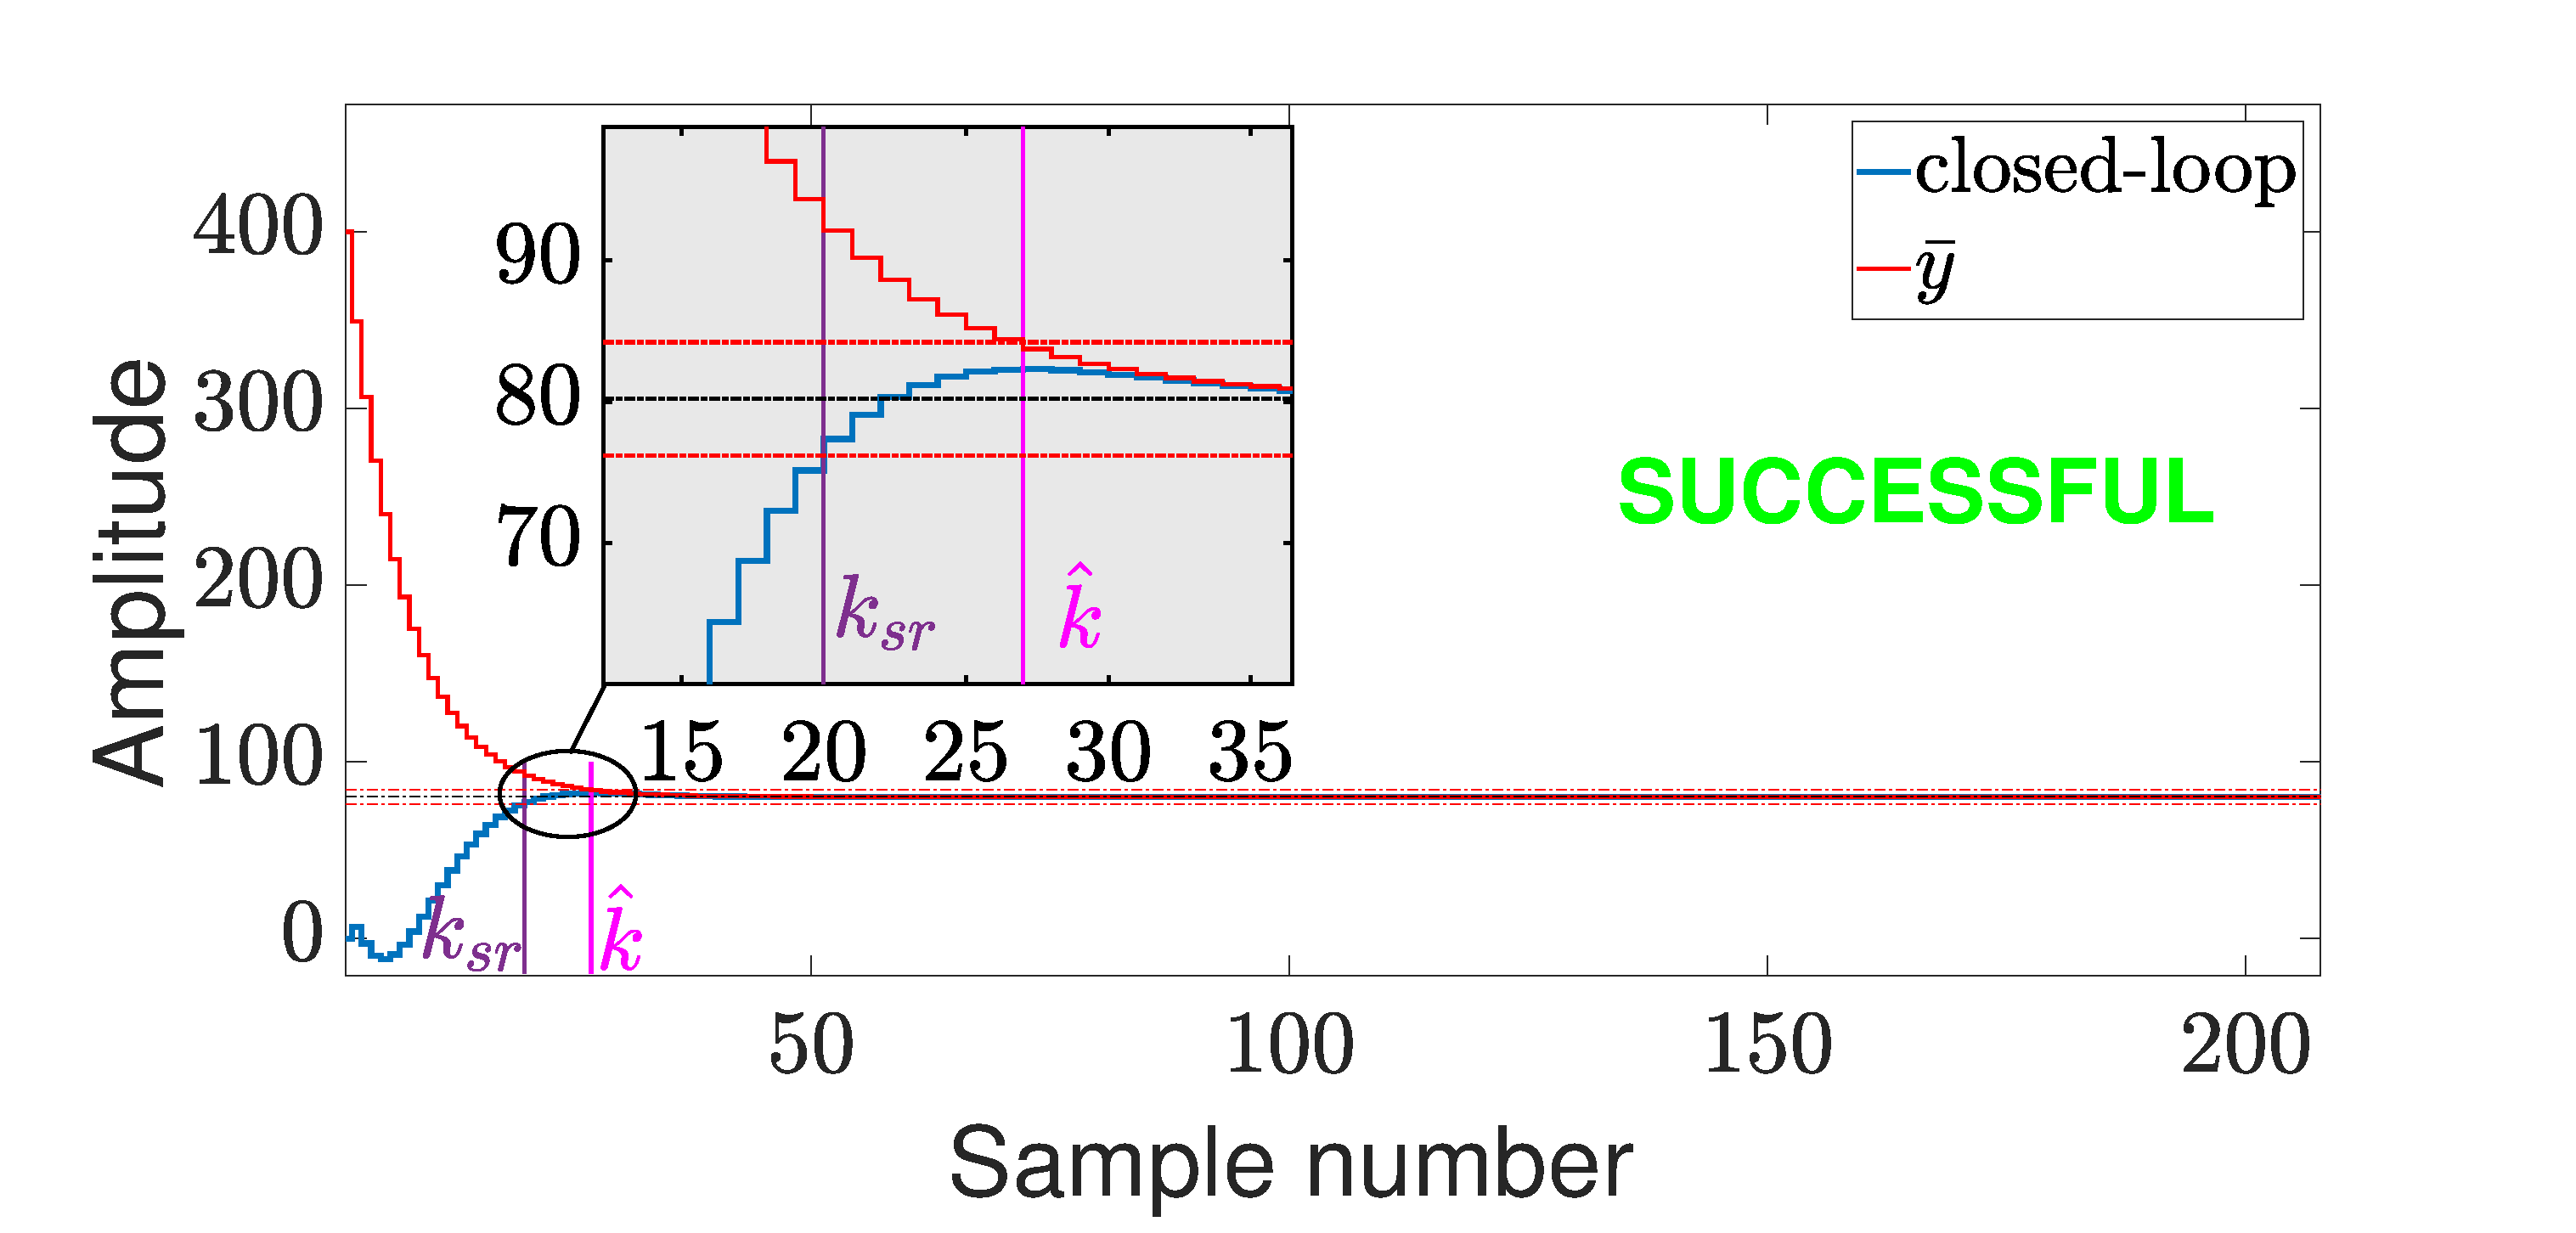
\includegraphics[trim={0.4cm 0cm 3cm 0cm}, clip,width=.4\textwidth]{figures/exDM13cl.eps}}\quad
   \subfloat[][]{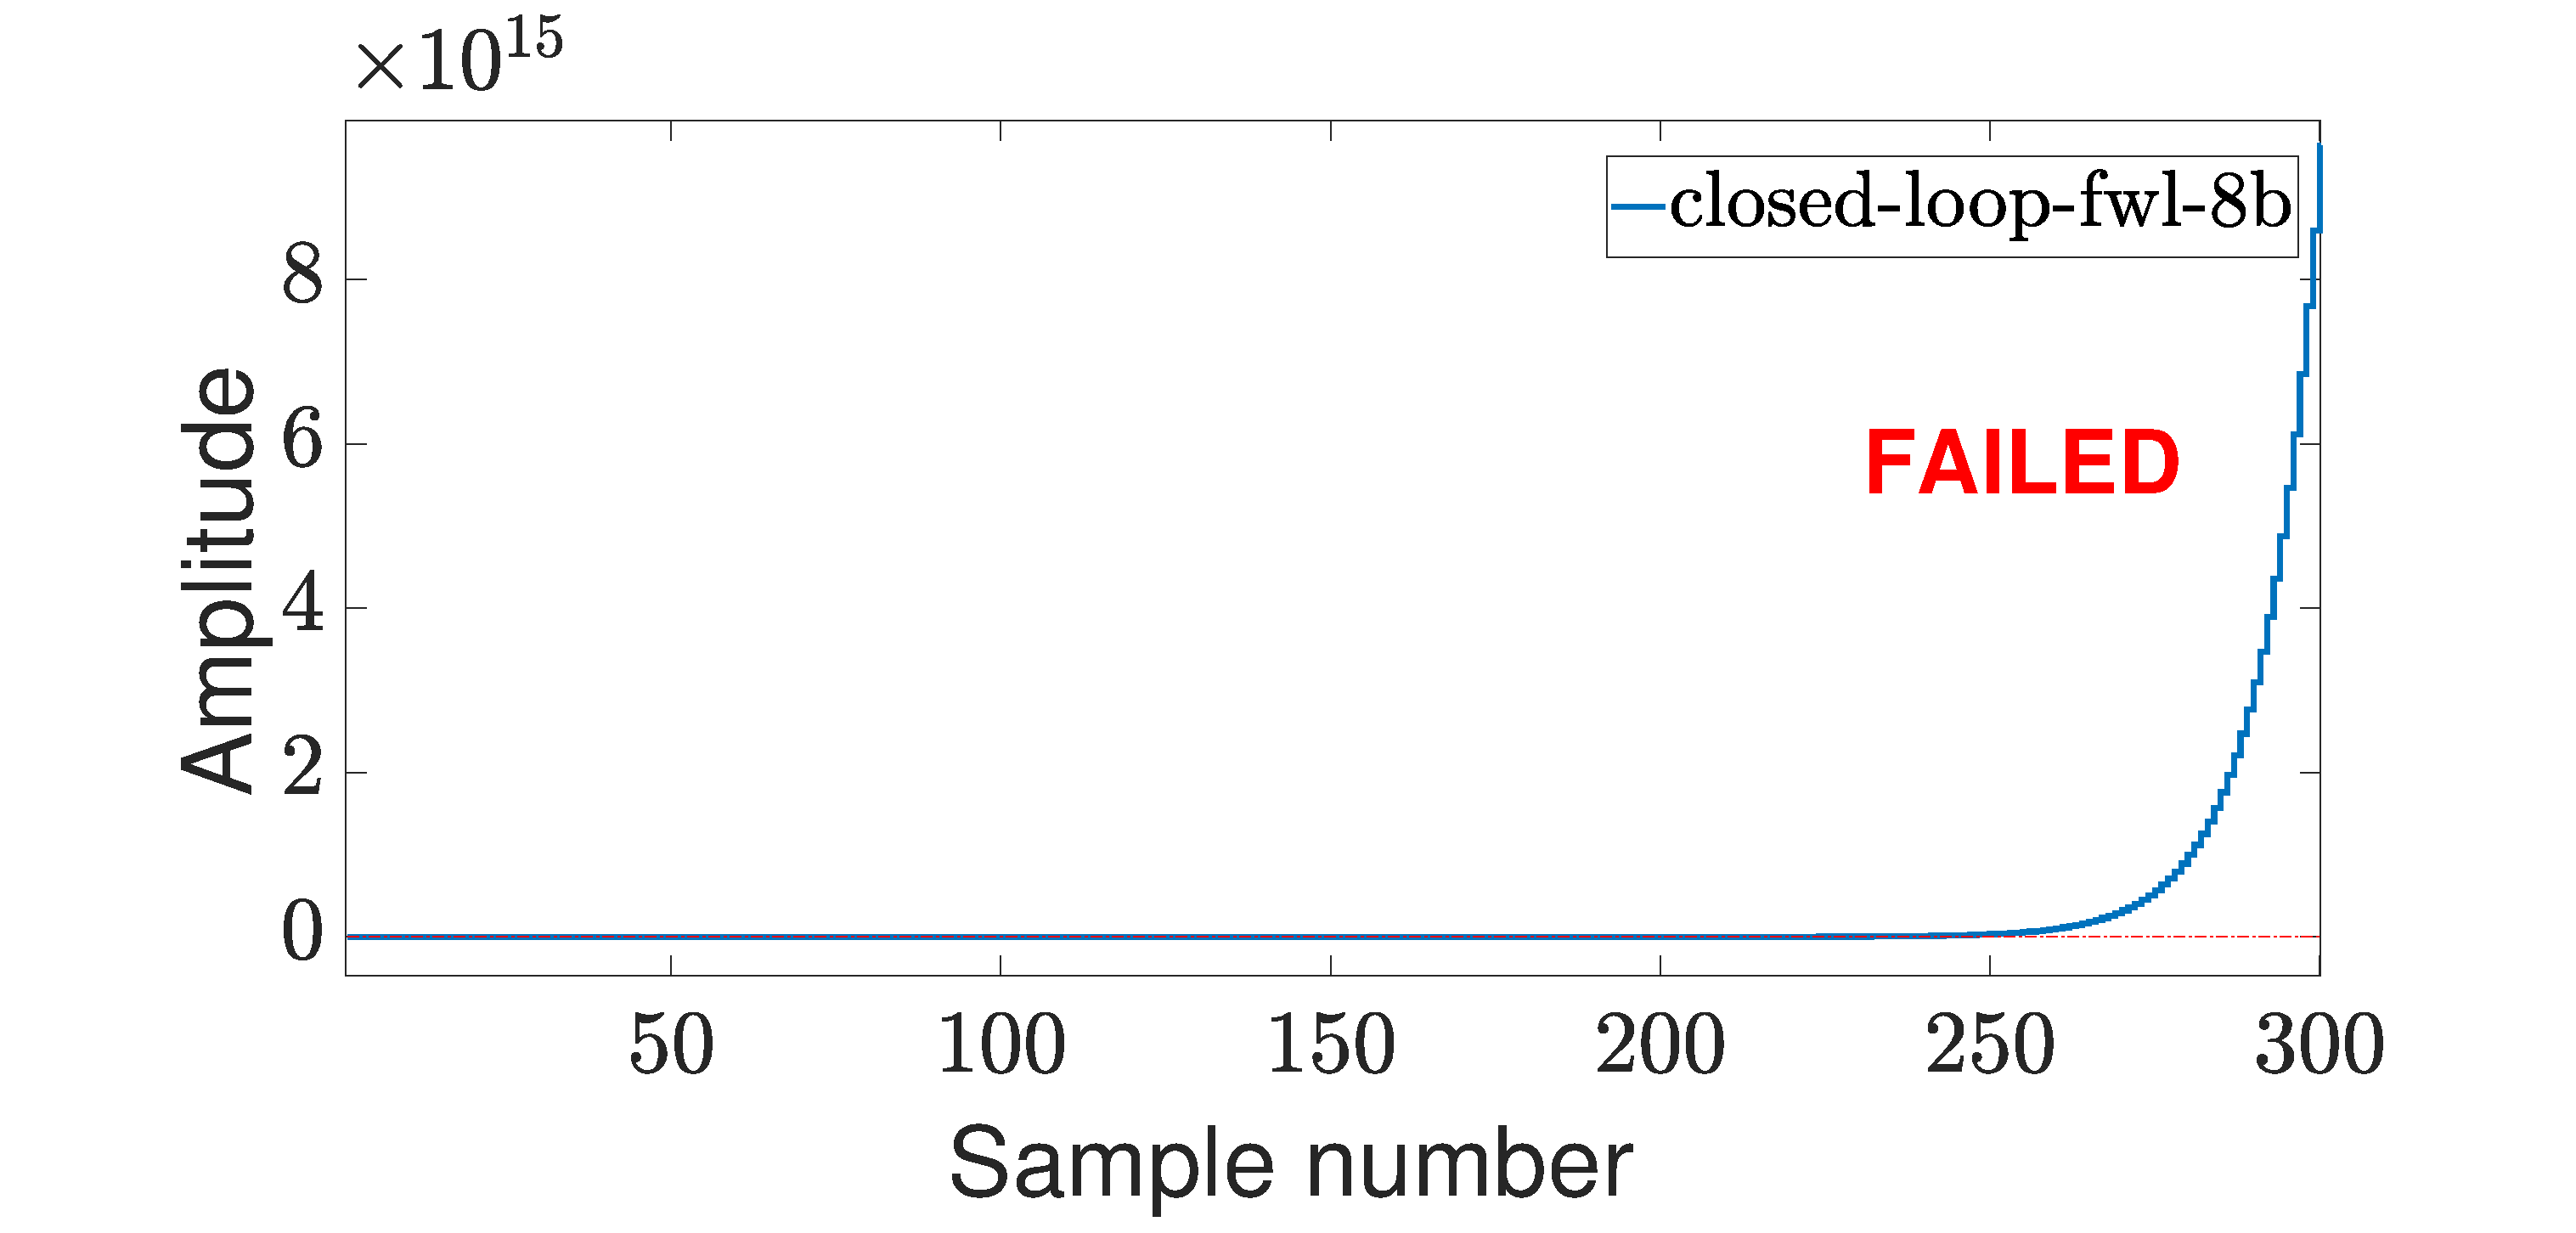
\includegraphics[trim={2cm 0cm 3cm 0cm}, clip,width=.4\textwidth]{figures/exDM13cl8b.eps}}\\
   \subfloat[][]{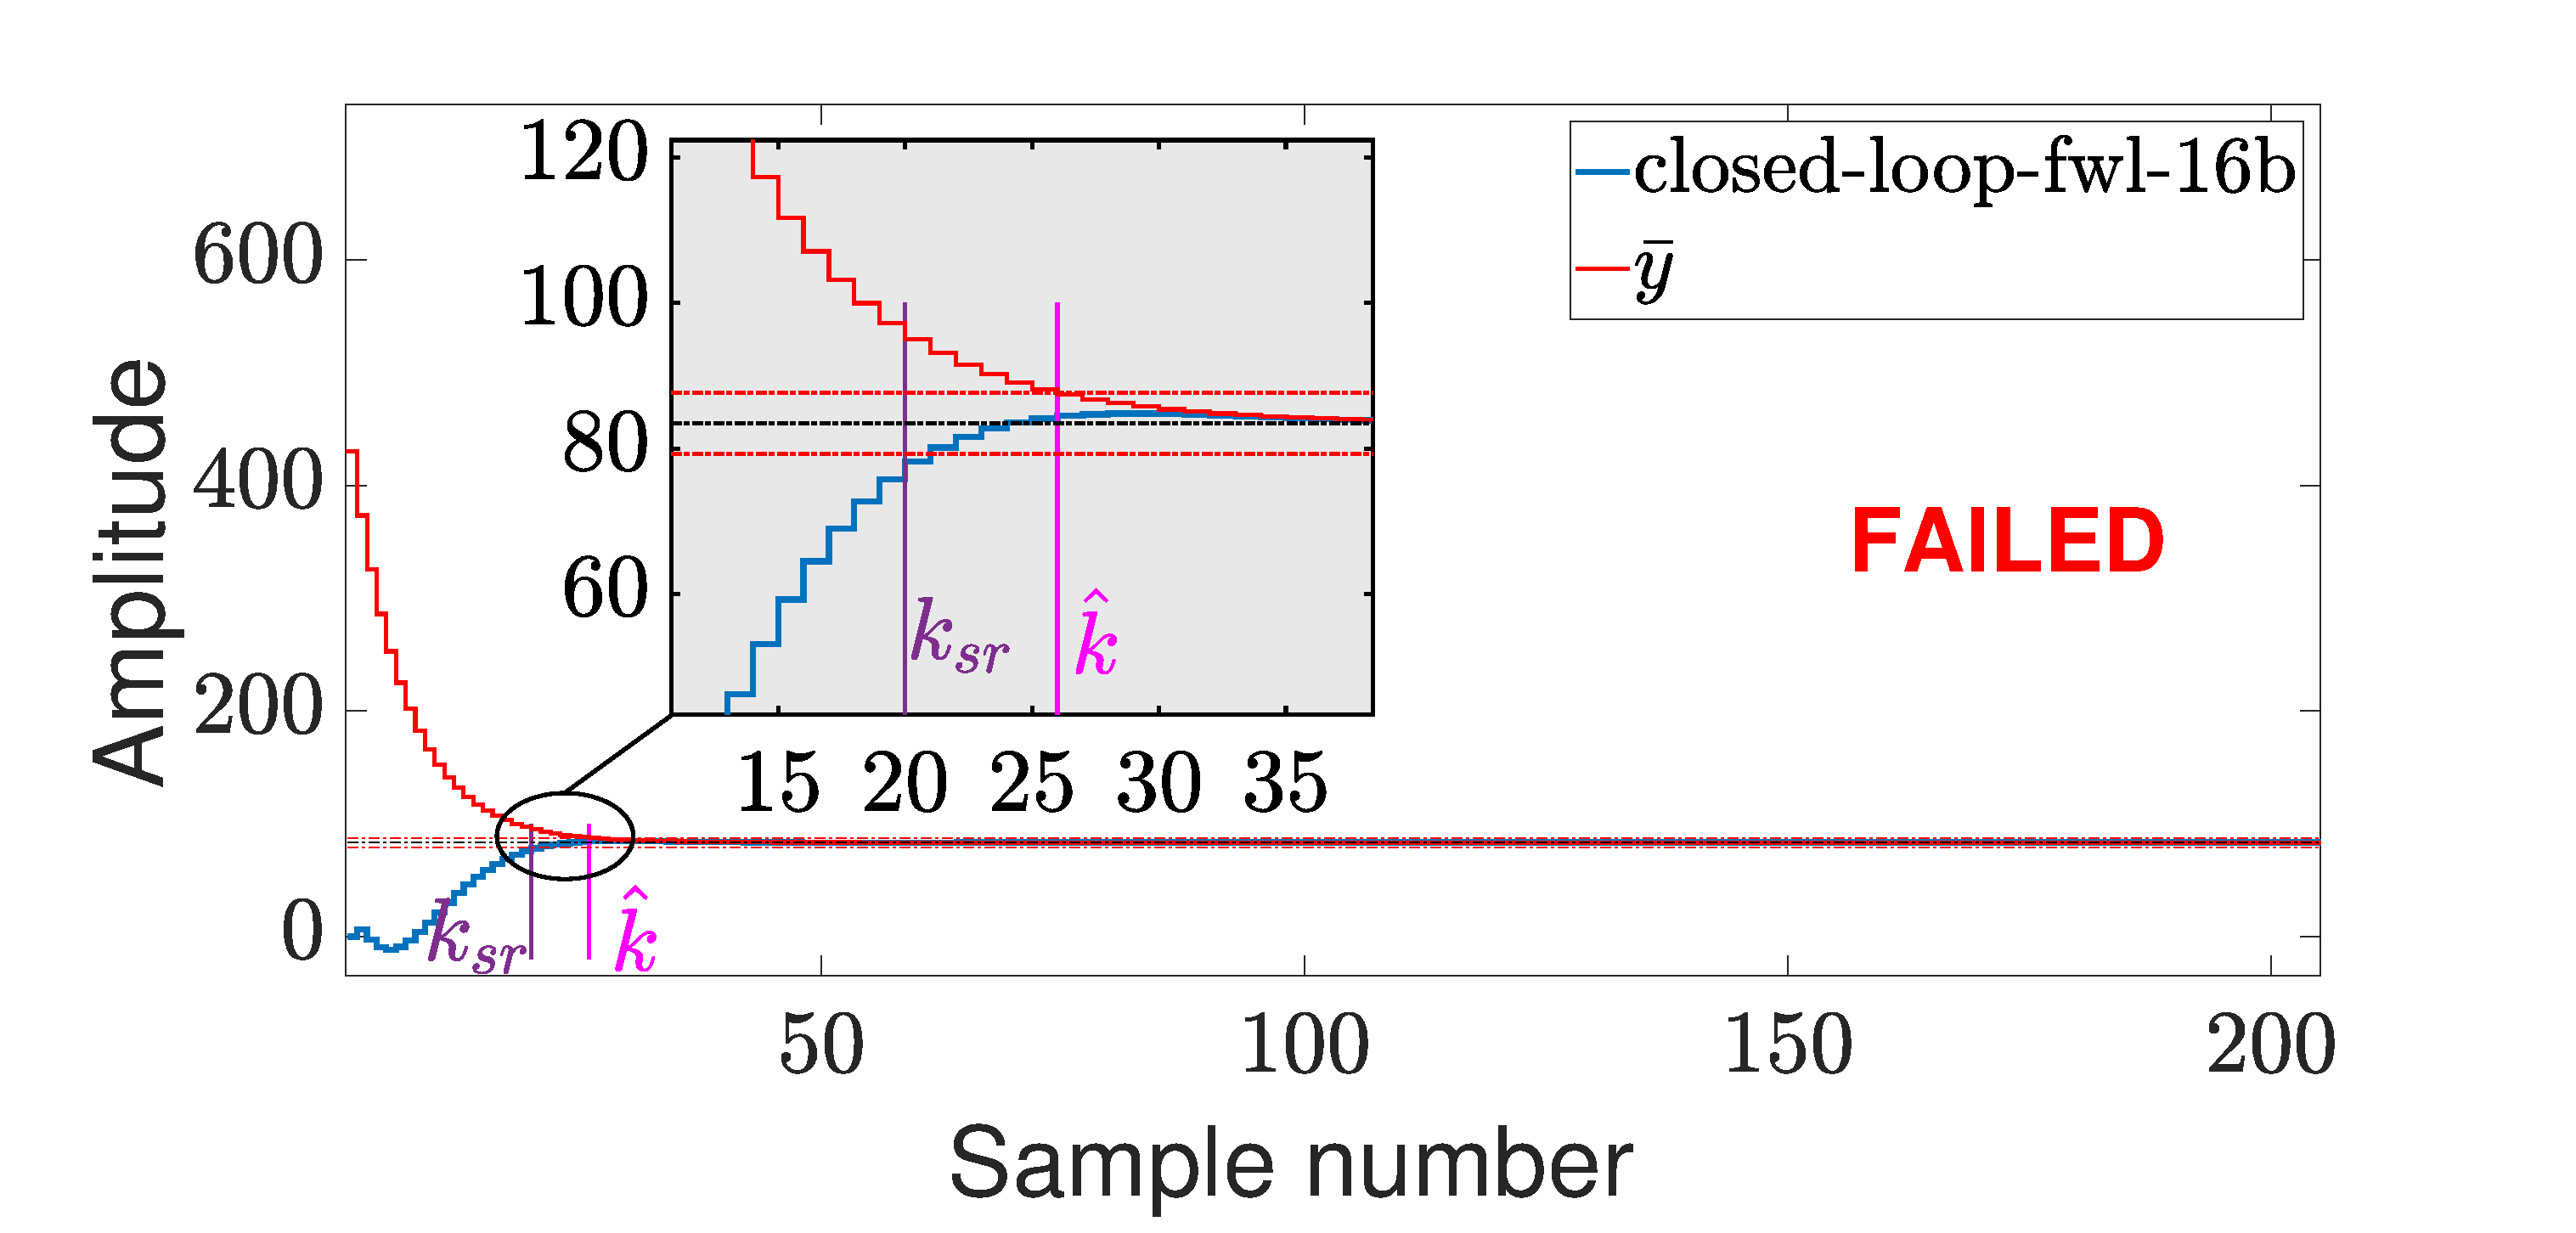
\includegraphics[trim={0.5cm 0cm 3cm 0cm}, clip,width=.4\textwidth]{figures/exDM13cl16b.eps}}\quad
   \subfloat[][]{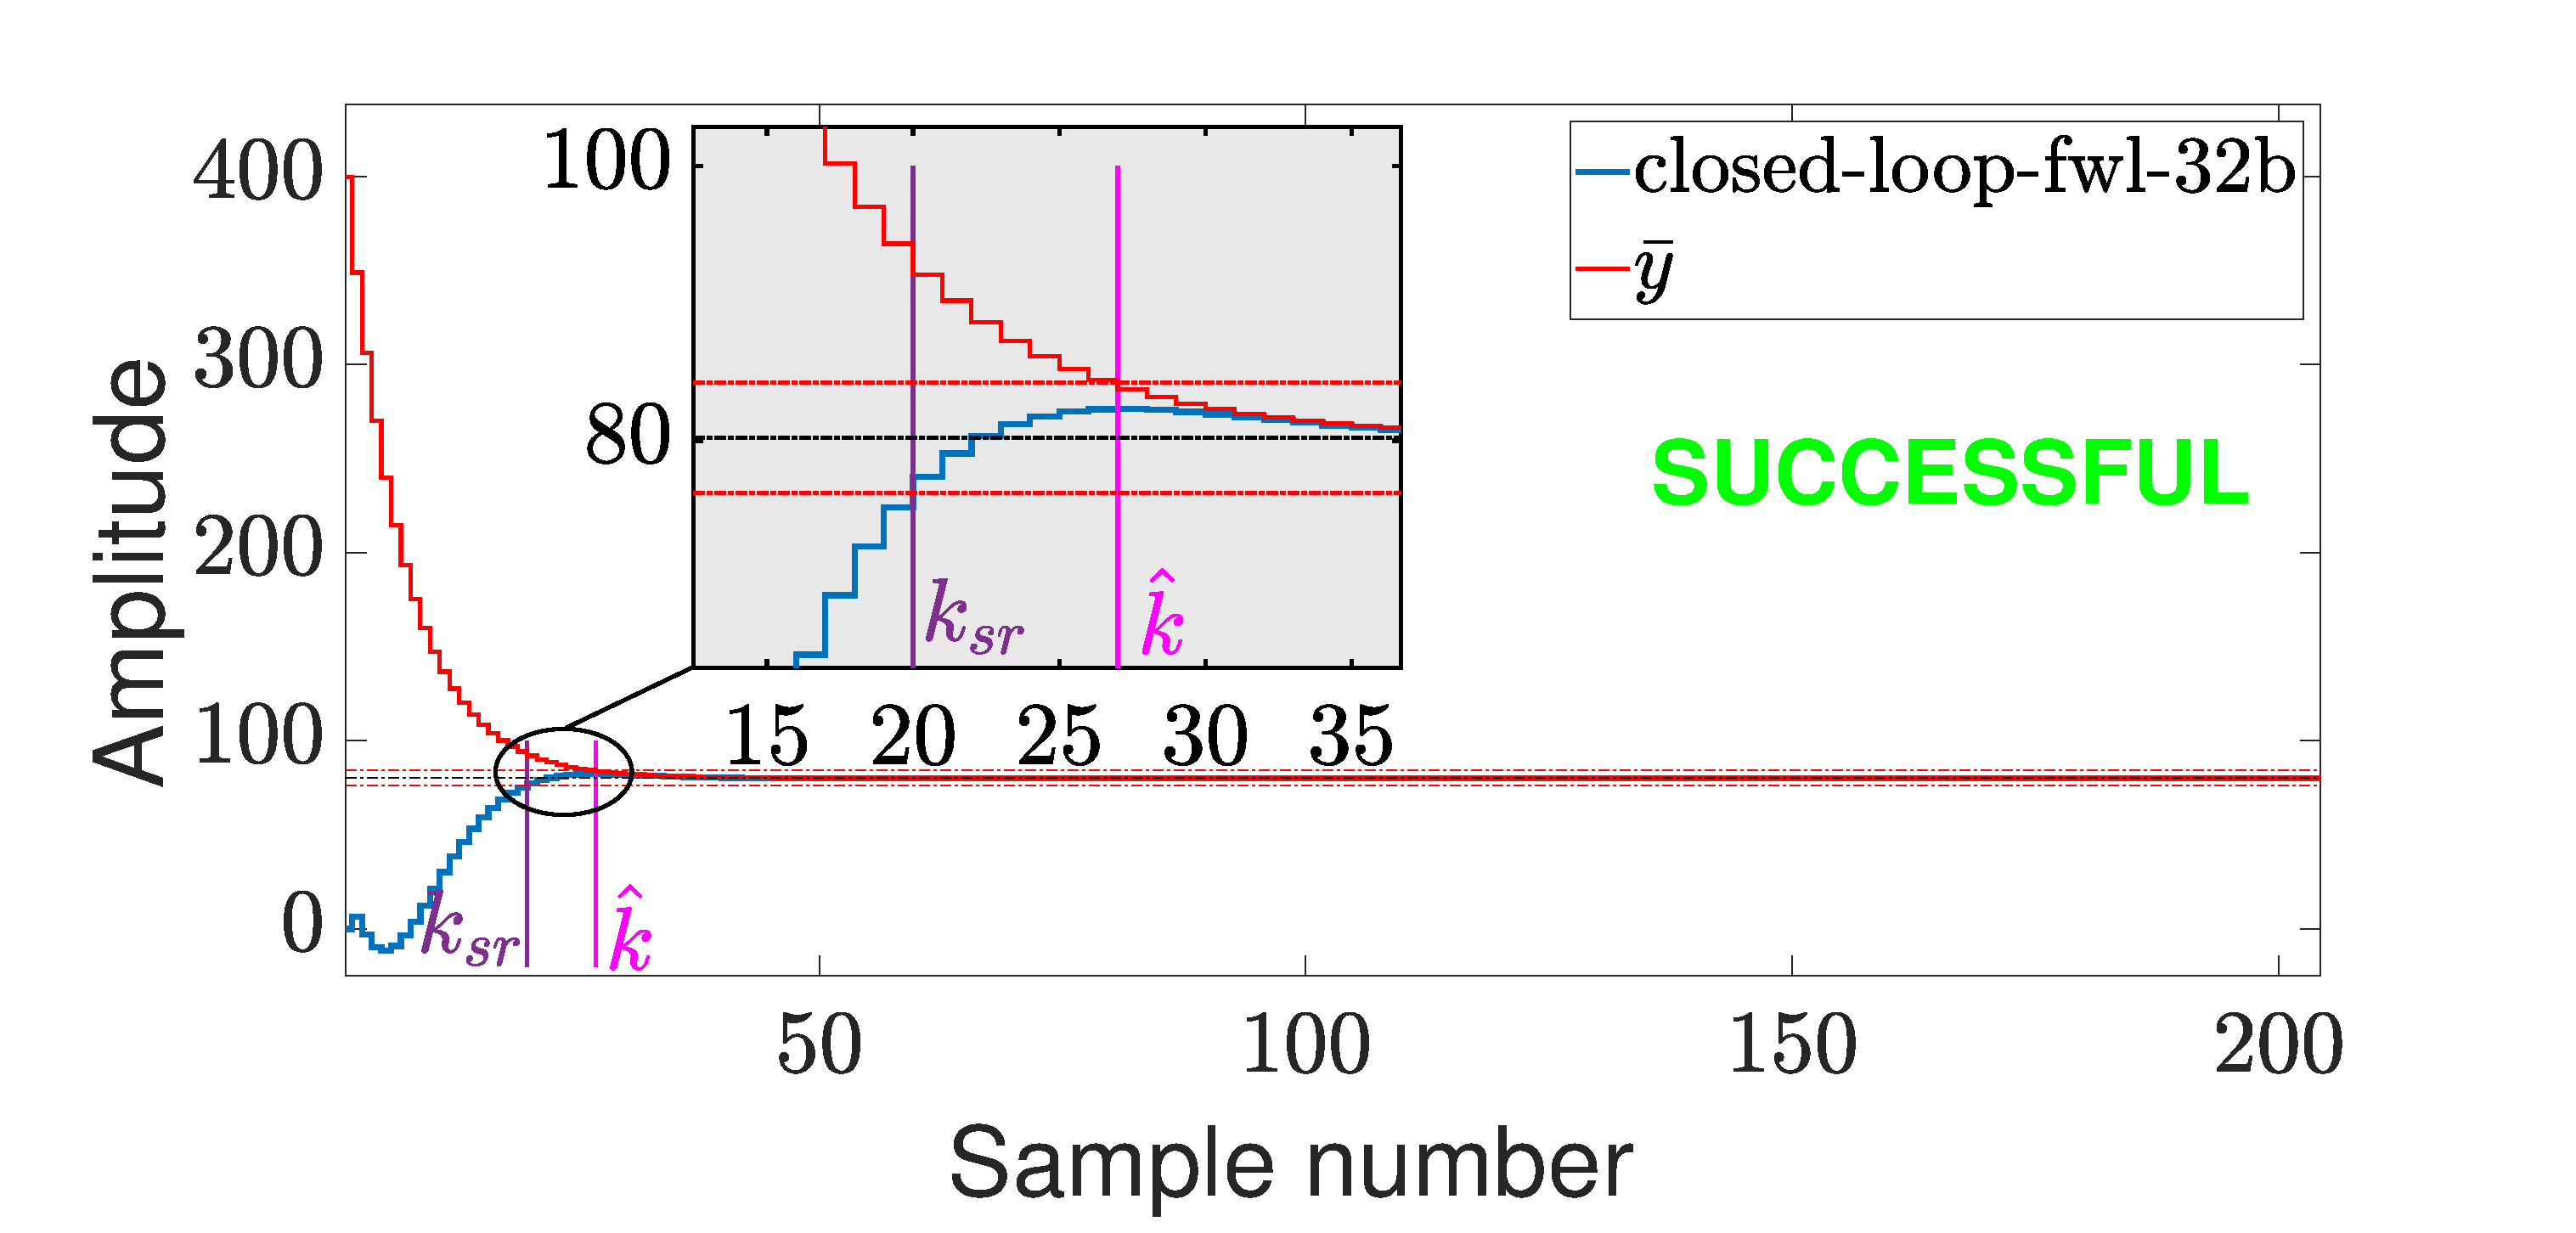
\includegraphics[trim={0.5cm 0cm 3cm 0cm}, clip,width=.4\textwidth]{figures/exDM13cl32b.eps}}
   \caption{Settling-time verification for the example system, (a) without FWL effects and with formats (b) $\langle 4,4 \rangle$, (c) $\langle 8,8 \rangle$, and (d) $\langle 16,16 \rangle$.
   }
   \label{fig:stmethod}
\end{figure}

The number of bits heavily influence settling-times in real implementations, due to FWL effects. In addition, ``\texttt{Verification FAILED}'' was obtained for an intermediate format $\langle 8,8 \rangle $, while it was successful with $\langle 16,16 \rangle $. Indeed, given that the resulting settling-time is mostly dependent on the fastest natural response and its damping ratio \cite{boyd1991linear}, the interaction between them after quantization may cause such a behavior, which further reinforces the use of the proposed methodology, during design phases.

One may also notice that the properties tackled during design phases are also modified, due to changes in coefficients and computation results. In particular, overshoot was affected in different ways, which means that if a property fails, the other may not, as can be seen for format $\langle 8,8 \rangle $.


One may notice that $t_{\mathrm{sr}}=10s$ is the sample $n=20$, discretized at $T_{\mathrm{s}}=0.5s$. Figure~\ref{fig:stmethod}(a) shows that $k_{\mathrm{sr}}=t_{\mathrm{sr}}/T_{\mathrm{s}}=20$ is less than the calculated $\hat{k}=37$ (Eq.~\ref{eq:kbar}) and, as a consequence, for this required settling-time, the system is already in the settling time region, so that settling-time is doable in that case. Finally, the same reasoning is valid for Figures~\ref{fig:stmethod}(b), (c) and (d), where we can analyze responses and check them according to Algorithm~\ref{alg:settlingtime}.

%-------------------------------------------------------------------
\section{Synthesis of Non-fragile Performance Specification Requirements}
\label{sec:synthesis}
%-------------------------------------------------------------------

In this section, we show our proposed synthesis methodology based on performance specification requirements for digital control systems. In particular, we analyze settling-time and maximum overshoot specifications, for digital state-feedback control systems. The proposed synthesis approach, which employs our verification methodologies for settling-time and overshoot, as explained in Sections~\ref{subsec:overshootAlg} and \ref{subsec:settime-alg}, is based on the CEGIS synthesis technique, where there are two stages: verification and learning (where the synthesizer is located) as we can see in Figure~\ref{fig:cegisDiag}. In the learning stage, we generate a controller $K$ in order to satisfy our required parameter (settling-time and/or overshoot), using genetic algorithms~\cite{deb2004introduction}, where we take the system's definitions and the requirements as constraints. After generating the controller $K$, there is the verification stage where it gets the controller $K$ and verifies if meets the requirements, according to our verification methodologies, and if it fails in that stage, it goes back to learning stage and keep work in that loop, until it get success in the verification or the synthesizer reaches a maximum number of attempts.

In Figure~\ref{fig:SynthArch}, we show the proposed synthesis architecture in a general form, where system definitions represent the system as a whole (state-space matrices, inputs, etc), requirements are the requirements to be synthesized, \texttt{total\_attempts} is the total number of attempts of synthesize a controller, \texttt{attempts} represents the number of attempts without change any synthesis parameter (genetic algorithm), GA is the block that performs the generation of a candidate controller though genetic algorithm (GA), \texttt{verify()} is the verification engine (Sections~\ref{subsec:overshootAlg} and \ref{subsec:settime-alg}) which rely on what we are synthesizing (settling-time and/or overshoot), \texttt{MAXATT} is the maximum number of attempts to synthesize a controller (informed by the user), \texttt{MAXINNERATT} represents the maximum number of attempts without change any GA parameter, \texttt{popsize} is the population size of the genetic algorithm and \texttt{STEP} is the step to increment the GA population.

\begin{figure}[ht]
\begin{center}
\includegraphics[trim={0.0cm 0.0cm 0.0cm 0cm}, clip,width=0.35\textwidth]{figures/FlowchartArch.eps}
\caption{Proposed synthesis architecture.} 
\label{fig:SynthArch}
\end{center}
\end{figure}

Our proposed synthesis methodology works as follows. We first define the system to be synthesized (plant, inputs, etc) and the requirements to be met (settling-time/overshoot), and then we choose what we want meet in the synthesis process. Additionaly, we run the genetic algorithm using the required constraints (settling-time and/or overshoot), so we generate a candidate controller $K$. Now, we perform the verification process (according to the property we chose to synthesize); if the verification has success, the synthesis is successfuly and it finishes the process. Otherwise the verification fails and we check if the total number of attempts exceeded the maximum number of attempts, if yes, the synthesis process fails and it finishes, contrarily, we check if the number of attempts without change any GA parameter exceeded the maximum number defined for that, if no it goes back to run the GA again (and continues the process again), on the other hand, we increment the population size of the GA, by a step fixed, and after that we re-execute the GA and continue the process again.

%\begin{tikzpicture}[node distance=1cm]
%\node (start) [startstop] {Start};
%\node (in1) [io, below of=start,align=left] {total\_attempts = 0 \\ inner\_attempts = 0};
%\node (proc1) [process, below of=in1] {GA};
%\node (proc2) [io, below of=proc1,align=left] {total\_attempts++ \\ inner\_attempts++};
%\node (dec1) [decision, below of=proc2, yshift=-0.5cm] {Verify};
%\node (dec2) [decision, below of=dec1, yshift=-0.5cm] {total\_attempts > MAX};
%\node (dec3) [decision, below of=dec2, yshift=-0.5cm] {inner\_attempts > MAX2};
%\node (proc3) [process, below of=dec3] {popsize \+\= steppop \\ inner\_attempts = 0};
%%\node (proc2a) [process, below of=dec1, yshift=-0.5cm] {Process 2a};
%%\node (proc2b) [process, below of=dec1, xshift=3cm, yshift=2.3cm] {Process 2b};
%\node (out1) [io, below of=dec1] {Output};
%\node (stop) [startstop, below of=out1] {Stop};
%\draw [arrow] (start) -- (in1);
%\draw [arrow] (in1) -- (proc1);
%\draw [arrow] (proc1) -- (proc2);
%\draw [arrow] (proc2) -- (dec1);
%\draw [arrow] (dec1) -- node[anchor=east] {yes} (out1);
%\draw [arrow] (dec1) -- node[anchor=south] {no} (dec2);
%\draw [arrow] (dec2) -| node[anchor=east] {yes} (out1);
%\draw [arrow] (dec2) -- node[anchor=east] {no} (dec3);
%\draw [arrow] (dec3) -- node[anchor=south] {yes} (proc3);
%\draw [arrow] (dec3) |- node[anchor=west] {yes} (proc1);
%\draw [arrow] (proc3) -- node[anchor=west] {} (proc1);
%\draw [arrow] (out1) -- (stop);
%
%
%
%\end{tikzpicture}



%--------------------------------------------------------------
\subsection{Generating candidate controller $K$}
\label{subsec:genK}
%--------------------------------------------------------------

In our CEGIS synthesis methodology, we use genetic algorithms to generate a candidate controller $K$, in order to satisfy the desired requirements (overshoot and settling-time). Our methodology uses a multi-objective functions to solve three separated problems: synthesize for overshoot, settling-time or both. The multi-objective functions are:
\begin{equation}
	\label{eq:objfuncSumK}
	\begin{array}{ccc}
		\mathbf{f}_\mathrm{1}(K)=K \times K^T\\
	\end{array}
\end{equation}

\noindent and

\begin{equation}
	\label{eq:objfuncST}
	\begin{array}{ccc}
		\mathbf{f}_\mathrm{2}(K)=\hat{k}\\
	\end{array}
\end{equation}

\noindent where $K$ is the controller matrix and $\hat{k}$ is given by Eq.~\ref{eq:kbar}.

\subsubsection{Optimization problem for overshoot}
\label{ssubsec:genKover}
With the goal of generating a controller matrix $K$ through genetic algorithms, in order to satisfy overshoot requirements, we have used the following problem formulation.

The optimization problem consists in minimizing $\mathbf{f}_\mathrm{1}$ and $\mathbf{f}_\mathrm{2}$ with respect to the decision variable $K$. Thus, the optimization problem is represented as follows:
%
\begin{equation}
	\label{eq:optproblemOS}
	\begin{array}{ccc}
		\min & (\mathbf{f}_\mathrm{1}(K),\mathbf{f}_\mathrm{2}(K)),  \\
  \\
		\textrm{ s.t. } & PO \leq PO_{\mathrm{r}}, \\
                        & \bar{\lambda} \leq 1      
 \\
	\end{array}
\end{equation}

The first constraint means that the actual percentage overshoot must be smaller than the required percentage overshoot ($PO_{r}$. The second constraint is related to system's stability, where $\bar{\lambda}$ is the maximum absolute value among the system's eigenvalues (Section~\ref{sec:modformver}) and this value must be smaller than $1$, otherwise, the system is unstable.

\subsubsection{Optimization problem for settling-time}
\label{ssubsec:genKst}

We formulate an optimization problem to generate $K$ in order to satisfies settling-time requirements.

The optimization problem consists in minimizing $\mathbf{f}_\mathrm{1}$ and $\mathbf{f}_\mathrm{2}$ with respect to the decision variable $K$. Thus, the optimization problem is represented as follows:
%
\begin{equation}
	\label{eq:optproblemST}
	\begin{array}{ccc}
		\min & (\mathbf{f}_\mathrm{1}(K),\mathbf{f}_\mathrm{2}(K)),  \\
  \\
		\textrm{ s.t. } & {\hat{k}} \leq k_{\mathrm{sr}}, \\
                        & \bar{\lambda} \leq 1
 \\
	\end{array}
\end{equation}

In this optimization problem, the first constraint means that $\hat{k}$ must be smaller than the required settling-time in discrete-time ($k_{sr}$, because as we can see in Algorithm~\ref{alg:settlingtime}, when that happens the verification is successful which mean that the system meets the required settling-time. The second constraint is related to system's stability, where $\bar{\lambda}$ is the maximum absolute value among the system's eigenvalues (Section~\ref{sec:modformver}) and this value must be smaller than $1$, otherwise, the system is unstable.

\subsubsection{Optimization problem to meet overshoot and settling-time}
\label{ssubsec:genKovst}

In order to generate a controller $K$ using genetic algorithm that satisfies both overshoot and settling-time requirements, we formulate the following optimization problem.

\begin{equation}
	\label{eq:optproblemOVST}
	\begin{array}{ccc}
		\min & (\mathbf{f}_\mathrm{1}(K),\mathbf{f}_\mathrm{2}(K)),  \\
  \\
		\textrm{ s.t. } & {\hat{k}} \leq k_{\mathrm{sr}}, \\
                        & PO \leq PO_{\mathrm{r}}, \\
                        & \bar{\lambda} \leq 1
 \\
	\end{array}
\end{equation}

In this case, we want no minimize hte multi-objective functions ($\mathbf{f}_\mathrm{1}$ and $\mathbf{f}_\mathrm{2}$) constrained to: $\hat{k} \leq k_\mathrm{sr}$, $PO \leq PO_{\mathrm{r}}$ and $\bar{\lambda} \leq 1$. The first constraint garantee that the system meets the settling-time requirement, since $ k_\mathrm{sr} \geq \hat{k}$ (cf. Algorithm~\ref{alg:settlingtime}). The second constraint assure the maximum percentage overshoot required (cf. Algorithm~\ref{alg:overshootReal}).  Finally, the third constraint ensure that controller $K$ will keep the system stable, in consideration of $\bar{\lambda}$ being the largest absolute eigenvalue and that being smaller than $1$ provides stability.

\section{Resumo}\label{chap-4-summary}

Neste cap�tulo foi apresesentado o m�todo proposto para localizar falhas em programas concorrentes usando t�cnicas de verifica��o de modelos e sequencializa��o, sendo esta a contribui��o maior do presente trabalho. Foi dada uma explica��o detalhada das transforma��es necess�rias, assim como um exemplo para ilustrar melhor o processo de localiza��o de falhas. Mostrou-se tamb�m a import�ncia do contraexemplo obtido antes da aplica��o do m�todo proposto, visto que o mesmo cont�m a ordem das {\it threads} executadas e os pontos onde trocas de contexto ocorreram. A modelagem necess�ria para transformar declara��es de programa concorrentes em sequenciais tamb�m foi explicada, assim como a estrutura fixa necess�ria para reproduzir a mesma ordem de execu��o do programa original. Por fim, um m�todo sequencial pode ser aplicado no novo c�digo para obter as linhas que levam �s falhas do programa. Como resultado, tem-se o embasamento para a avalia��o experimental realizada no pr�ximo cap�tulo.

\chapter{Resultados e Discuss�es}\label{chap_results}

Este cap�tulo est� dividido em tr�s partes. A primeira parte descreve os objetivos dos experimentos conduzidos neste trabalho. A segunda � dedicada � descri��o da configura��o na qual os experimentos foram realizados, m�quinas (processador e mem�ria RAM) e sistemas operacionais. A terceira apresenta os resultados obtidos quando se realizaram os experimentos com os \textit{benchmarks} selecionados, assim como uma discuss�o sobre os resultados obtidos e avalia��o geral do m�todo proposto nesta disserta��o.

\section{Objetivos do Experimento}\label{sec:experimental-objectives}

Utilizando os \textit{benchmarks} propostos, os experimentos t�m os seguintes objetivos:

\begin{enumerate}

\item Demonstrar a aplicabilidade da metodologia para a s�ntese de controladores digitais.

\item Avaliar as vantagens da metodologia comparada a outras existentes.

\end{enumerate}

\section{Configura��o Experimental e Descri��o dos \textit{Benchmarks}}\label{sec:experimental-setup}

Os experimentos foram conduzidos em m�quinas com diferentes configura��es, para acelerar a gera��o dos resultados. Parte foi executada em um processador Intel Core i$7$ -- $4500$ $1$.$8$GHz, com $32$ GB de RAM e executando sistema operacional Linux Mint $64$-bits. Outra parte foi executada em um processador Intel Core i$7$ -- $4500$ $1$.$8$GHz, com $16$ GB de RAM e executando sistema operacional Linux Ubuntu Server $64$-bits. Uma outra parte foi conduzida em um processador Intel Core i$7$ -- $7700$ $3$.$6$GHz, com $32$ GB de RAM e executando sistema operacional Linux Ubuntu $64$-bits. A ultima parte foi obtida em um processador Intel Core i$7$ -- $4500$ $1$.$8$Ghz, com $16$ GB de RAM e executando sistema operacional Linux Ubuntu $64$-bits.

Os benchmarks com os sistemas de controle usados para avaliar a abordagem proposta s�o descritos a seguir. Em particular, os benchmarks usados neste trabalho est�o dispon�veis na Tabela, e fornece informa��es sobre as matrizes de espa�o de estados $ \mathbf{A} $, $ \mathbf{B} $ e $ \mathbf{C} $, mais ou menos na forma can�nica de Jordan~\cite{chen1995linear}, tempo de assentamento requerido $t_{\mathrm{sr}}$ e porcentagem de sobressinal requerido $PO_{\mathrm{r}}$. Todos os benchmarks apresentam a matriz de espa�o de estados $ D = [0] $ e foram escolhidos porque abordam diferentes cen�rios em rela��o a autovalores de $ \mathbf{A} $. Existem sistemas de $ 2\textsuperscript{nd} $, $ 3\textsuperscript{rd} $, $ 4\textsuperscript{th} $ e $ 5\textsuperscript{th} $ ordem e um de auta ordem ($ 17\textsuperscript{th} $), com autovalores iguais,  diferentes, reais e complexos. Al�m disso, dois deles s�o exemplos do mundo real: o 15 representa uma planta f�sica real de um motor DC e o 16 descreve uma planta f�sica de levita��o magn�tica. Al�m disso, o benchmark 17 � um sistema de $ 17\textsuperscript{th} $ ordem baseado no fornecido por \cite{tran2016large} e depois discretizado. Os benchmarks utilizados em nosso estudo n�o cont�m sistemas MIMO (multiple-input multiple-output), uma vez que a metodologia proposta � capaz de verificar apenas os SISO, no momento.

H� $51$ experimentos considerando somente tempo de assentamento divididos em 3 diferentes configura��es de FWL ($ 8 $, $ 16 $ e $ 32 $ bits), mais $51$ exeperimentos considerando somente sobressinal, novamente dididos em 3 diferentes configura��es de FWL ($ 8 $, $ 16 $ e $ 32 $ bits). Tamb�m foram realizados $51$ experimentos considerando ambas as propriedades (tempo de assentamento e sobressinal) e incluindo novamente experimentos de 3 diferentes formatos de FWL ($ 8 $, $ 16 $ e $ 32 $ bits)


\section{Resultados Experimentais}\label{sec:experimental-results}

A Tabela~\ref{table:results} resume os resultados experimentais. ``\textbf{\#}'' descreve uma identifica��o do \textit{benchmark}, \textbf{R} representa resultado da s�ntese (bem ou mal sucedida), \textbf{T} � o n�mero de tentativas para realizar a s�ntese, \textbf{t} identifica o tempo levado para sintetizar um controlador, e, finalmente, $\langle 4,4 \rangle $, $\langle 8,8 \rangle $ e $\langle 16,16 \rangle $ representam o formato de FWL considerando, onde representam no total $8$, $16$ e $32$, respectivamente.

\begin{table}[ht]
\renewcommand{\arraystretch}{1.0}
\caption{Resultados dos experimentos}
\label{table:results}
\centering
%\footnotesize
%\scriptsize
%\tiny
\miniscule
\begin{tabular}{|c|c|c|c|c|c|c|c|c|c|c|c|c|c|c|c|c|c|c|c|c|c|c|c|c|c|c|c|}
\hline
\textbf{\#}       & \multicolumn{9}{c|}{\textbf{Tempo de Assentamento}}                                                                                                                               & \multicolumn{9}{c|}{\textbf{Sobressinal}}                                                                                                                                         & \multicolumn{9}{c|}{\textbf{Tempo de Assentamento e Sobressinal}}                                                                                                        \\ \hline
\multirow{2}{*}{} & \multicolumn{3}{c|}{\textit{$\langle 4,4 \rangle $}}      & \multicolumn{3}{c|}{\textit{$\langle 8,8 \rangle $}}      & \multicolumn{3}{c|}{\textit{$\langle 16,16 \rangle $}}    & \multicolumn{3}{c|}{\textit{$\langle 4,4 \rangle $}}      & \multicolumn{3}{c|}{\textit{$\langle 8,8 \rangle $}}      & \multicolumn{3}{c|}{\textit{$\langle 16,16 \rangle $}}    & \multicolumn{3}{c|}{$\langle 4,4 \rangle $}      & \multicolumn{3}{c|}{\textit{$\langle 8,8 \rangle $}}      & \multicolumn{3}{c|}{\textit{$\langle 16,16 \rangle $}}    \\ \cline{2-28} 
                  & \textit{\textbf{R}} & \textit{\textbf{T}} & \textit{\textbf{t}} & \textit{\textbf{R}} & \textit{\textbf{T}} & \textit{\textbf{t}} & \textit{\textbf{R}} & \textit{\textbf{T}} & \textit{\textbf{t}} & \textit{\textbf{R}} & \textit{\textbf{T}} & \textit{\textbf{t}} & \textit{\textbf{R}} & \textit{\textbf{T}} & \textit{\textbf{t}} & \textit{\textbf{R}} & \textit{\textbf{T}} & \textit{\textbf{t}} & \textit{\textbf{R}} & \textit{\textbf{T}} & \textit{\textbf{t}} & \textit{\textbf{R}} & \textit{\textbf{T}} & \textit{\textbf{t}} & \textit{\textbf{R}} & \textit{\textbf{T}} & \textit{\textbf{t}} \\ \hline
1                 &          S          &          1           &                &          S          &       1        &                &          S          &          3           &                &                    &                     &                &                    &                     &                &                    &                     &                &           &                     &                &                    &                     &                &                    &                     &                \\ \hline
2                 &          S          &           1          &                &          S          &        1       &                &          S          &          4           &                &                    &                     &                &                    &                     &                &                    &                     &                &           &                     &                &                    &                     &                &                    &                     &                \\ \hline
3                 &          S          &           1          &                &          S          &        2        &                &          S          &          2           &                &                    &                     &                &                    &                     &                &                    &                     &                &           &                     &                &                    &                     &                &                    &                     &                \\ \hline
4                 &          S          &           1          &                &          S          &        1        &                &          S          &          1           &                &                    &                     &                &                    &                     &                &                    &                     &                &           &                     &                &                    &                     &                &                    &                     &                \\ \hline
5                 &          S          &           1          &                &          S          &        1        &                &          S          &          7           &                &                    &                     &                &                    &                     &                &                    &                     &                &           &                     &                &                    &                     &                &                    &                     &                \\ \hline
6                 &          S          &           1          &                &          S          &        5        &                &          S          &          41           &                &                    &                     &                &                    &                     &                &                    &                     &                &           &                     &                &                    &                     &                &                    &                     &                \\ \hline
7                 &          S          &           1          &                &          S          &        1        &                &          S          &          1           &                &                    &                     &                &                    &                     &                &                    &                     &                &           &                     &                &                    &                     &                &                    &                     &                \\ \hline
8                 &          S          &           1          &                &          S          &        1        &                &          S          &          3           &                &                    &                     &                &                    &                     &                &                    &                     &                &           &                     &                &                    &                     &                &                    &                     &                \\ \hline
9                 &          S          &           1          &                &          S          &        1        &                &          S          &          3           &                &                    &                     &                &                    &                     &                &                    &                     &                &           &                     &                &                    &                     &                &                    &                     &                \\ \hline
10                &          S          &           3          &                &          S          &        2        &                &          S          &          6           &                &                    &                     &                &                    &                     &                &                    &                     &                &           &                     &                &                    &                     &                &                    &                     &                \\ \hline
11                &                    &                     &                &                    &                     &                &                    &                     &                &                    &                     &                &                    &                     &                &                    &                     &                &           &                     &                &                    &                     &                &                    &                     &                \\ \hline
12                &                    &                     &                &                    &                     &                &                    &                     &                &                    &                     &                &                    &                     &                &                    &                     &                &           &                     &                &                    &                     &                &                    &                     &                \\ \hline
13                &                    &                     &                &                    &                     &                &                    &                     &                &                    &                     &                &                    &                     &                &                    &                     &                &           &                     &                &                    &                     &                &                    &                     &                \\ \hline
14                &                    &                     &                &                    &                     &                &                    &                     &                &                    &                     &                &                    &                     &                &                    &                     &                &           &                     &                &                    &                     &                &                    &                     &                \\ \hline
15                &                    &                     &                &                    &                     &                &                    &                     &                &                    &                     &                &                    &                     &                &                    &                     &                &           &                     &                &                    &                     &                &                    &                     &                \\ \hline
16                &                    &                     &                &                    &                     &                &                    &                     &                &                    &                     &                &                    &                     &                &                    &                     &                &           &                     &                &                    &                     &                &                    &                     &                \\ \hline
17                &                    &                     &                &                    &                     &                &                    &                     &                &                    &                     &                &                    &                     &                &                    &                     &                &           &                     &                &                    &                     &                &                    &                     &                \\ \hline
\multicolumn{28}{|l|}{\textbf{S} = S�ntese bem sucedida e \textbf{F} = S�ntese mal sucedida}
\\ \hline
\end{tabular}
\end{table}



\subsection{Compara��o com Outras T�cnicas de Projeto de Controladores Digitais}
\label{sec:comparison-controller-design}

Algumas abordagens de projeto de controladores digitais s�o utilizados por engenheiros de controle, alguns deles foram mostrados na Se��o~\ref{sec:tpcsd}. Agora mostraremos uma compara��o de algumas dessas t�cnicas com a empregada neste trabalho, frente a um problema de controle do mundo real.

O modelo que utilizaremos � o \textit{benchmark} $14$ da Tabela~\ref{table:bench}.

\subsubsection{Aloca��o de Polos}
\label{sec:alopol}
Usando a t�cnica de aloca��o de polos, conforme descrito em \eqref{subsec:ap}, temos que,

Primeiramente obtemos o polin�mio caracter�stico da matriz $\mathbf{A}$ e aplicamos na Equa��o~\ref{eq:matrixQ}, para obter a matrix $\mathbf{P}$, que �

\begin{equation*}
P=10^6 \times \begin{bmatrix}
   -2.2464 &  -0.0337  &  0.9006  &  0.0135 \\
   -2.2464 &  -0.0112  &  0.8984  &  0.0045 \\
   -2.2464 &   0.0112  &  0.8984  & -0.0045 \\
   -2.2464 &   0.0337  &  0.9006  & -0.0135 
\end{bmatrix}
\end{equation*}

\noindent Agora, calculamos o polin�mio caracter�stico dos autovalores desajados para obter a matrix $\bar{K}$,

\begin{equation*}
\bar{K}=\begin{bmatrix}
    0.2629 &  -0.7552  &  0.7233  & -0.2309
\end{bmatrix}
\end{equation*}

\noindent com isso, podemos calcular o controlador $\mathbf{K}$,

\begin{equation*}
\mathbf{K}=\bar{K}P= \begin{bmatrix}
  -61.9933 & -33.5040 &  95.0597 &  18.8300
\end{bmatrix}
\end{equation*}

Esse controlador, quando aplicado ao sistema, faz com que obtenhamos o comportamento que desejamos, que � um tempo de assentamento pr�ximo a $t_\mathrm{sr}=$ e $PO_\mathrm{r}=$.

A resposta do sistema � mostrada na Figura.


\subsubsection{Regulador Quadr�tico Linear}
\label{sec:regqudLin}
Como objetivo de projetar um controlador utilizando a t�cnica do regulador quadr�tico linear, usamos a metodologia implementada pelo Matlab~\cite{guide1998mathworks} que consiste em minimizar  a fun��o de custo $J(u)=\sum_{n=1}^\infty \left( x[n]^TQx[n]+u[n]^TRu[n]+2x[n]^TNu[n] \right)$ para o sistema em tempo discreto em \eqref{eq:ssed}.

Al�m do ganho de realimenta��o de estado $\mathbf{K}$, a metodologia implementada pelo Matlab retorna a solu��o de horizonte infinito $S$ da equa��o Riccati de tempo discreto associada~\cite{bittanti2012riccati}. O controlador $\mathbf{K}$ � derivado de $S$ por $\mathbf{K} = (B^TSB + R)^{-1}(B^TSA + N^T)$, onde obtivemos $\mathbf{K}=[  -61.9933 ~ -33.5040 ~  95.0597  ~ 18.8300]$. Com isso, obtivemos uma resposta do sistema conforme desej�vamos, como pode ser visto na Figura.



\subsubsection{Sintonia Autom�tica}
\label{sec:sinaut}


\subsection{Aplicando a Abordagem Proposta na Pr�tica}
\label{sec:method-in-practice}


\subsection{Considera��es Finais}
\label{sec:final-considerations}

%Os benchmarks aplicados basicamente apresentam um tipo de erro: bloqueios fatais, assertivas, aquisi��o de sem�foros, divis�o por zero, seguran�a de ponteiros, estouro aritm�tico, ou viola��o de limites de vetores. Logo, aplicaram-se diferentes regras, dependendo da falha detectada. A Figura~\ref{figure:summary-verification-results} mostra um resumo de todos os resultados obtidos, o qual mostra que a metodologia proposta gera informa��es �teis sobre execu��es mal-sucedidas, com rela��o ao erro presente no benchmark, em $84$.$21$\% dos benchmarks utilizados, al�m de identificar quais linhas est�o relacionadas � falha associada e quais valores podem ser atribu�dos para produzir uma execu��o bem-sucedida. Com rela��o aos benchmarks utilizados, a abordagem n�o foi capaz de diagnosticar linhas defeituosas em tr�s deles, devido � modelagem da biblioteca concorrente do C, visto que tais benchmarks apresentaram problemas de bloqueios fatais e sincroniza��o.
%
%\begin{figure*}[htb]
%\centering
%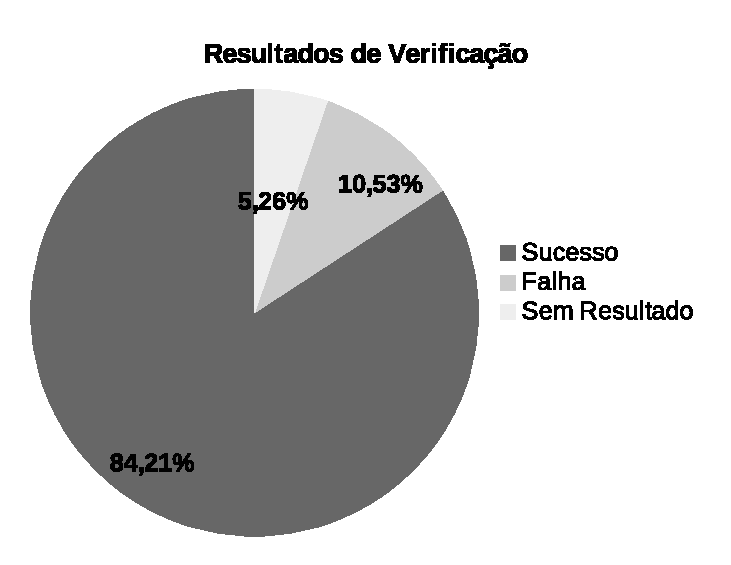
\includegraphics[scale=0.75]{figures/verification_results}
%\caption{Resumo dos resultados de verifica��o}
%\label{figure:summary-verification-results}
%\end{figure*}
%
%A Figura~\ref{figure:summary-verification-time} mostra um resumo do tempo de verifica��o necess�rio para cada benchmark. Treze programas levaram menos de $2$ segundos, de forma a avaliar as falhas existentes e as atribui��es associadas para produzir uma execu��o bem-sucedida, tr�s programas n�o foram verificados corretamente, com tempos associados de verifica��o menores que  $2$ segundos, e, finalmente, tr�s benchmarks levaram cerca de $4$ a $5$ vezes mais para produzir resultados �teis. Com rela��o ao �ltimo caso, analizando o processo de verifica��o do verificador de modelos, foi poss�vel apontar o gargalo como sendo o solucionador SMT, devido � quantidade de fontes de n�o-determinismo presentes em tais benchmarks. No entanto, o tempo de verifica��o em m�dia ainda � baixo, se comparado com o que pode ser obtido com depura��o de programas n�o-assistida~\cite{Mayer:2008}.
%
%\begin{figure*}[htb]
%\centering
%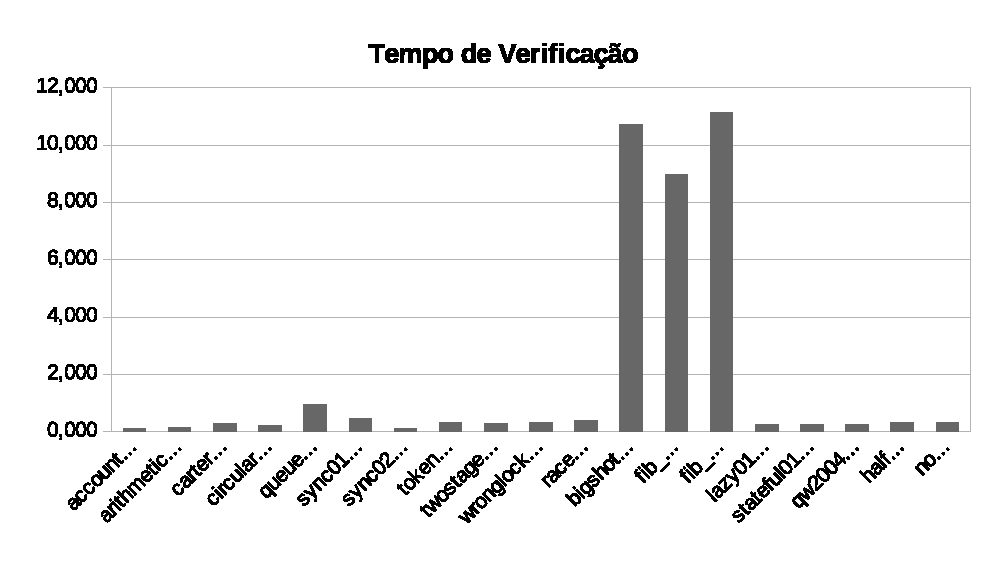
\includegraphics[scale=0.75]{figures/verification_time}
%\caption{Resumo dos resultados de todos os benchmarks}
%\label{figure:summary-verification-time}
%\end{figure*}
%
%Em resumo, os resultados apresentados mostram que a metodologia proposta � apropriada para localizar falhas em programas concorrentes em C, e que o tempo de verifica��o necess�rio para produzir uma execu��o bem-sucedida do programa � curto. Logo, a metodologia proposta pode ser �til para auxiliar desenvolvedores a depurar programas.

\section{Resumo}\label{chap-5-summary}

%Neste cap�tulo apresentou a avalia��o experimental realizada para o m�todo proposto neste trabalho, assim como considera��es a serem feitas sobre a metodologia apresentada. O experimento foi conduzido com um computador padr�o e os dados obtidos foram analizados, mostrando a viabilidade do m�todo para encontrar linhas defeituosas em c�digos concorrentes, tendo uma taxa de sucesso de $84$.$21$\%, considerando todos os benchmarks propostos. A metodologia proposta mostrou-se �til para determinar as linhas defeituosas em um programa concorrente. No entanto, a depend�ncia de um contraexemplo para iniciar o processo de transforma��o de c�digo levou a alguns benchmarks n�o serem avaliados, pois o ESBMC n�o foi capaz de retornar um contraexemplo para os mesmos. Tamb�m � importante notar que ap�s a transforma��o de c�digo ser feita, o tempo de verifica��o do c�digo instrumentado foi sempre menor que $1$ segundo. De modo geral, a metodologia garante que a corre��o no c�digo original das linhas obtidas nos contraexemplos do novo c�digo sequencial levam a uma execu��o bem-sucedida do programa.

\chapter{Conclus�es}\label{chap_conclusion}

\section{Considera��es Finais}

Nesta disserta��o foi apresentado uma metodologia de s[intese, bem como verifica��o de controladores digitais, considerando os efeitos de FWL na implementa��o de controladores. Como parte do processo de s�ntese, a verifica��o foi realizada de maneira formal, onde verificamos requisitos de desempenho como tempo de assentamento e sobressinal. Como parte do processo de s�ntese, a gera��o de candidatos, no caso controladores candidatos, foi feito atrav�s de problemas de otimiza��o resolvido com algoritmo gen�tico.

%Com rela��o aos resultados experimentais, a metodologia proposta foi capaz de identificar potenciais falhas em software concorrente, em $84$.$21$\% dos benchmarks escolhidos, enquanto falhou em obter linhas defeituosas �teis em tr�s dos benchmarks adotados. De fato, um deles apresentou um bloqueio fatal e os outros dois falham devido a problemas de sincroniza��o de \textit{threads}, o que necessita de uma investiga��o mais a fundo, de forma a prover aprimoramentos relacionados �s abordagens de modelagem das primitivas de sincroniza��o do C. No entanto, o m�todo � �til para avaliar programas concorrentes que apresentam falhas relacionadas a assertivas mal-formuladas e bloqueios fatais, o que o torna interessante para auxiliar desenvolvedores a encontrar atribui��es que levem a execu��es bem-sucedidas de programas e, consequentemente, minimiza o esfor�o em depura��o de c�digo.
%
%Ao ser comparado com outras abordagens, o m�todo proposto � capaz de localizar falhas em programas concorrentes usando apenas o c�digo-fonte do programa, ao inv�s de um caminho mal-sucedido e uma su�te de teste. Ele tamb�m � capaz de n�o somente apontar as linhas defeituosas, como tamb�m prover poss�veis consertos para produzir execu��es bem-sucedidas do programa.
%
%Durante o desenvolvimento deste trabalho foram identificados pontos que diminuem a efici�ncia do m�todo proposto. Dentre esses pontos, tamb�m observados na avalia��o experimental, pode-se destacar a necessidade de um contraexemplo para a posterior aplica��o do m�todo, dependendo inteiramente da capacidade do verificador de modelos de encontrar viola��es no programa original. Este problema est� relacionado diretamente � tarefa de custo mais elevado no m�todo proposto, que � a defini��o do vetor \texttt{cs}. Uma defini��o arbrit�ria, por meio de uso de t�cnicas de BMC, pode ser estudado em trabalhos posteriores.
%
%Outro ponto a se considerar � a modelagem de estruturas da biblioteca {\it pthread}. Internamente, o ESBMC implementa um modelo para as primitivas de sincroniza��o da biblioteca, e neste trabalho define-se uma modelagem em um n�vel anterior � tradu��o interna do ESBMC. Deve-se tamb�m investigar qual das duas modelagens deve ser adotada com o objetivo de melhorar os resultados obtidos.
%
%Apesar dos pontos descritos anteriormente, quando se trata do m�todo proposto para localizar falhas, o tempo de verifica��o � curto (geralmente menor que $1$ segundo) para o programa sequencial instrumentado n�o-determin�stico, possibilitando um diagn�stico r�pido para o mesmo.
%
%De maneira geral, pode-se concluir que os objetivos espec�ficos desta disserta��o tamb�m foram atingidos.
%
%Em uma empresa de desenvolvimento de software � comum o uso de programa��o concorrente para prover solu��es com tempo menor de resposta. Por�m, esta classe de programas est� sujeita a erros mais dif�ceis de serem corrigidos, e por consequ�ncia, erros que levem mais tempo para serem encontrados. O uso de um m�todo para localizar falhas em tais programas reduziria drasticamente o tempo associado a esta tarefa, melhorando o processo de desenvolvimento de software concorrente. O m�todo proposto nesta disserta��o visa ser uma alternativa para depura��o comum, usando uma t�cnica tamb�m em ascens�o para busca por defeitos, a verifica��o de modelos.

\section{Propostas para Trabalhos Futuros}

Nesta se��o ser�o apresentadas algumas propostas para desenvolvimentos futuros relacionados � metodologia proposta descrita nesta disserta��o. As propostas podem ser divididas em dois tipos de melhorias. A primeira � relacionada a parte de verifica��o e a segunda a s�ntese em si.

%Quanto ao problema de sequencializa��o e modelagem de c�digo:
%
%\begin{itemize}
%
%\item Novas regras para transforma��o devem ser adicionadas para que seja poss�vel representar melhor o programa original em rela��o �s intercala��es entre as {\it threads} existentes.
%
%\item Melhorias na gram�tica para que seja poss�vel diagnosticar melhor problemas relacionados a declara��es relacionadas � biblioteca {\it pthread}.
%
%\item O uso de desdobramento de la�os para melhor representa��o de la�os existentes em programas concorrentes, onde tamb�m podem existir trocas de contexto.
%
%\end{itemize}
%
%Quanto ao problema de aplicabilidade do m�todo em geral:
%
%\begin{itemize}
%
%\item Um {\it plugin} deve ser desenvolvido em um ambiente de desenvolvimento, como o {\it Eclipse}, de forma a automatizar o processo de localiza��o de falhas.
%
%\item Propor uma estrat�gia para simular todas as intercala��es poss�veis, retirando o processo de defini��o do escalonamento definido em c�digo do verificador de modelos.
%
%\item Incorporar a abordagem proposta por Gadelha {\it et al.}~\cite{Nicole:2017} para minimizar o esfor�o necess�rio para encontrar um contraexemplo para um programa concorrente defeituoso.
%
%\item Aplicar o m�todo em outros seguimentos de programas, {\it e.g.}, programas concorrentes em Qt~\cite{Monteiro:2017}.
%
%\end{itemize}


\bibliographystyle{abntex2-num}
\bibliography{references/references}

\appendix

\chapter{Publica��es}

\section{Referente � Pesquisa}

\begin{itemize}

\item \textbf{Alves, E. H. S.}, Cordeiro, L. C., Lima Filho, E. B. {\it Fault Localization in Multi-Threaded C Programs using Bounded Model Checking}. Em V Simp�sio Brasileiro de Engenharia de Sistemas Computacionais (SBESC), 2015. (\textbf{Publicado})~\cite{AlvesCF15}

\item \textbf{Alves, E. H. S.}, Cordeiro, L. C., Lima Filho, E. B. {\it A Method to Localize Faults in Concurrent C Programs}. Em \textit{Journal of Software and Systems}, 2017. (\textbf{Publicado})~\cite{AlvesCF17}

\end{itemize}

\section{Contribui��es em outras Pesquisas}

\begin{itemize}
\item Cavalcante, T. R. F., \textbf{Alves, E. H. S.}, Carvalho, C. B. \textit{Radio Communication to Control and Run an Autonomous Mission for UAVs via a Mobile Application}. Em IV Escola Regional de Inform�tica (ERIN), 2017. (\textbf{Publicado})
\item Monteiro, F. R. M., \textbf{Alves, E. H. S.}, Silva, I. S., Ismail, H. I., Cordeiro, L. C., Lima Filho, E. B. \textit{ESBMC-GPU A Context-Bounded Model Checking Tool to Verify CUDA Programs}. Em \textit{Science of Computer Programming}, 2018. (\textbf{Publicado})~\cite{MonteiroASICF18}
\end{itemize}

\chapter{\textit{Benchmarks} Utilizados}\label{appendix:bench}

\begin{table}[ht]
\centering
%\centering
\caption{Descri��o dos \textit{benchmarks} usados nos experimentos do trabalho.}
\label{table:bench}
\footnotesize
\resizebox{0.9\textwidth}{!}{%
\begin{tabular}{l|ccccc|c}
\hline
\textbf{ID} & \textbf{$A$}                                                                                                                                                         & \textbf{$B$}                                                                 & \textbf{$C$}                                                              & \textbf{$K$}                                                                            & \textbf{$t_{\mathrm{sr}}$ (s)}
& \textbf{$PO_{\mathrm{r}}$} \\ \hline
1           & $ \begin{bmatrix}
-0.5 & 1.0 \\
0.0 & -0.5 
\end{bmatrix}  $ & $ \begin{bmatrix}
0.0 \\
2.5 
\end{bmatrix} $                                                              & $ \begin{bmatrix}
0.0 & 2.6 
\end{bmatrix} $                                                                                                                        & $ \begin{bmatrix}
0.3641 & -0.7161 
\end{bmatrix} $                                                                     & 2.5 & 5              \\
2           & \begin{tabular}[c]{@{}c@{}}$ \begin{bmatrix}
-0.5 & 1.0 & 0.0 \\
0.0 & -0.5 & 1.0 \\
0.0 & 0.0 & -0.5 
\end{bmatrix}  $\end{tabular}                                                                              & \begin{tabular}[c]{@{}c@{}}$ \begin{bmatrix}
-0.4 \\
2.5 \\
-0.8 
\end{bmatrix} $                                                             \end{tabular}             & \begin{tabular}[c]{@{}c@{}}$ \begin{bmatrix}
0.0 & 2.6 & 0.0 
\end{bmatrix} $                                                             \end{tabular}            & \begin{tabular}[c]{@{}c@{}}$ \begin{bmatrix}
1.0706 \\ -0.0277 \\ 2.8996 
\end{bmatrix} ^ T $\end{tabular}                & 3.5     & 5          \\
3           & \begin{tabular}[c]{@{}c@{}}$ \begin{bmatrix}
-0.5 & 1.0 & 0.0 & 0.0 \\
0.0 & -0.5 & 1.0 & 0.0 \\
0.0 & 0.0 & -0.5 & 1.0 \\
0.0 & 0.0 & 0.0 & -0.5 
\end{bmatrix}  $\end{tabular}                                         & \begin{tabular}[c]{@{}c@{}}$ \begin{bmatrix}
1.0 \\
2.5 \\
1.0 \\
1.0 
\end{bmatrix} $                                                             \end{tabular}           & \begin{tabular}[c]{@{}c@{}}$ \begin{bmatrix}
0.0 & 2.6 & 1.2 & 0.0 \end{bmatrix} $                                                             \end{tabular}        & \begin{tabular}[c]{@{}c@{}}$ \begin{bmatrix}
0.444 \\ -2.6941 \\ 5.7609 \\ -2.8354 
\end{bmatrix} ^ T $\end{tabular}        & 4.5      & 30         \\
4           & \begin{tabular}[c]{@{}c@{}}$ \begin{bmatrix}
-0.5 & 1.0 & 0.0 & 0.0 & 0.0 \\
0.0 & -0.5 & 1.0 & 0.0 & 0.0 \\
0.0 & 0.0 & -0.5 & 1.0 & 0.0 \\
0.0 & 0.0 & 0.0 & -0.5 & 1.0 \\
0.0 & 0.0 & 0.0 & 0.0 & -0.5 
\end{bmatrix}  $\end{tabular} & \begin{tabular}[c]{@{}c@{}}$ \begin{bmatrix}
-0.4 \\
-0.6 \\
5.5 \\
1.0 \\
-0.3 
\end{bmatrix} $                                                             \end{tabular} & \begin{tabular}[c]{@{}c@{}}$ \begin{bmatrix}
0.0 & 2.6 & 0.5 & 1.2 & 0.0 \end{bmatrix} $                                                             \end{tabular} & \begin{tabular}[c]{@{}c@{}}$ \begin{bmatrix}
0.5811 \\ -2.5168 \\ 15.458 \\ -14.5328 \\ 251.9519 
\end{bmatrix} ^ T $\end{tabular} & 5.5          & 20     \\
5           & $ \begin{bmatrix}
-0.5 & 0.4 \\
-0.4 & -0.5 
\end{bmatrix}  $                                                                                                                                           & $ \begin{bmatrix}
0.0 \\
2.5 
\end{bmatrix} $                                                                                                                           & $ \begin{bmatrix}
0.0 & 2.6 \end{bmatrix} $                                                                                                                        & $ \begin{bmatrix}
0.8725 & -0.7848 
\end{bmatrix} $                                                                       & 3.0    & 5           \\
6           & \begin{tabular}[c]{@{}c@{}}$ \begin{bmatrix}
-0.5 & 0.4 & 1.0 & 0.0 \\
-0.4 & -0.5 & 0.0 & 1.0 \\
0.0 & 0.0 & -0.5 & 0.4 \\
0.0 & 0.0 & -0.4 & -0.5 
\end{bmatrix}  $\end{tabular}                                       & \begin{tabular}[c]{@{}c@{}}$ \begin{bmatrix}
0.0 \\
0.0 \\
2.5 \\
1.6 
\end{bmatrix} $                                                             \end{tabular}           & \begin{tabular}[c]{@{}c@{}}$ \begin{bmatrix}
0.0 & 2.6 & 0.0 & 2.0 \end{bmatrix} $                                                             \end{tabular}        & \begin{tabular}[c]{@{}c@{}}$ \begin{bmatrix}
-0.3248 \\ 0.804 \\ 0.694 \\ -3.2113 
\end{bmatrix} ^ T $\end{tabular}         & 5.0    & 30           \\
7           & \begin{tabular}[c]{@{}c@{}}$ \begin{bmatrix}
-0.5 & 0.4 & 0.0 & 0.0 \\
-0.4 & -0.5 & 0.0 & 0.0 \\
0.0 & 0.0 & -0.8 & 0.4 \\
0.0 & 0.0 & -0.4 & -0.8 
\end{bmatrix}  $\end{tabular}                                       & \begin{tabular}[c]{@{}c@{}}$ \begin{bmatrix}
-0.4 \\
-0.6 \\
2.5 \\
1.6 
\end{bmatrix} $                                                             \end{tabular}         & \begin{tabular}[c]{@{}c@{}}$ \begin{bmatrix}
0.0 & 2.6 & 0.0 & 2.0 \end{bmatrix} $                                                             \end{tabular}        & \begin{tabular}[c]{@{}c@{}}$ \begin{bmatrix}
14.8068 \\ -5.2354 \\ 4.9214 \\ -8.8323 
\end{bmatrix}  ^ T $\end{tabular}         & 10.0          & 4    \\
8           & $ \begin{bmatrix}
-0.2 & 0.0 \\
0.0 & -0.3 
\end{bmatrix}  $                                                                                                                                            &$ \begin{bmatrix}
-0.6 \\
2.5 
\end{bmatrix} $                                                                                                                          & $ \begin{bmatrix}
0.0 & 2.6 
\end{bmatrix} $                                                                                                                        & $ \begin{bmatrix}
-2.5516 & -0.873 
\end{bmatrix} $                                                                                                                                    & 1.5         & 8      \\
9           & \begin{tabular}[c]{@{}c@{}}$ \begin{bmatrix}
-0.2 & 0.0 & 0.0 \\
0.0 & -0.3 & 0.0 \\
0.0 & 0.0 & -0.7 
\end{bmatrix}  $\end{tabular}                                                                            & \begin{tabular}[c]{@{}c@{}}$ \begin{bmatrix}
-0.8 \\
-0.7 \\
-0.5 
\end{bmatrix} $                                                             \end{tabular}            & \begin{tabular}[c]{@{}c@{}}$ \begin{bmatrix}
0.0 & 2.6 & 0.0 \end{bmatrix} $                                                             \end{tabular}            & \begin{tabular}[c]{@{}c@{}}$ \begin{bmatrix}
3.5127 \\
-8.0225 \\
9.4041 
\end{bmatrix} ^ T $\end{tabular}                    & 2.0       & 8        \\
10          & \begin{tabular}[c]{@{}c@{}}$ \begin{bmatrix}
-0.2 & 0.0 & 0.0 & 0.0 \\
0.0 & -0.3 & 0.0 & 0.0 \\
0.0 & 0.0 & -0.7 & 0.0 \\
0.0 & 0.0 & 0.0 & -0.9 
\end{bmatrix}  $\end{tabular}                                         & \begin{tabular}[c]{@{}c@{}}$ \begin{bmatrix}
-0.4 \\
2.5 \\
1.0 \\
-0.7
\end{bmatrix} $                                                             \end{tabular}         & \begin{tabular}[c]{@{}c@{}}$ \begin{bmatrix}
0.0 & 2.6 & 1.2 & 0.0 \end{bmatrix} $                                                             \end{tabular}        & \begin{tabular}[c]{@{}c@{}}$ \begin{bmatrix}
-8.6418 \\
-3.8839 \\
37.21 \\
49.6053 
\end{bmatrix} ^ T $\end{tabular}               & 5.0       & 30        \\
11          & \begin{tabular}[c]{@{}c@{}}$ \begin{bmatrix}
-0.2 & 0.0 & 0.0 & 0.0 & 0.0 \\
0.0 & -0.3 & 0.0 & 0.0 & 0.0 \\
0.0 & 0.0 & -0.7 & 0.0 & 0.0 \\
0.0 & 0.0 & 0.0 & -0.9 & 0.0 \\
0.0 & 0.0 & 0.0 & 0.0 & -0.5 
\end{bmatrix}  $\end{tabular} & \begin{tabular}[c]{@{}c@{}}$ \begin{bmatrix}
-0.5 \\
-0.2 \\
2.5 \\
2.0 \\
-0.8
\end{bmatrix} $                                                             \end{tabular} & \begin{tabular}[c]{@{}c@{}}$ \begin{bmatrix}
0.0 & 2.6 & 0.5 & 1.2 & 0.0 \end{bmatrix} $                                                             \end{tabular} & \begin{tabular}[c]{@{}c@{}}$ \begin{bmatrix}
34.4436 \\
-382.0806 \\
143.6879 \\
-91.9969 \\
299.8048 
\end{bmatrix} ^ T $\end{tabular}   & 10.0    & 18          \\
12          & $ \begin{bmatrix}
4.5 & 1.0 \\
0.0 & 4.5 
\end{bmatrix}  $ & $ \begin{bmatrix}
0.0 \\
2.5 
\end{bmatrix} $                                                                                                                           & $ \begin{bmatrix}
0.0 & 2.6 
\end{bmatrix} $                                                                                                                        & $ \begin{bmatrix}
5.5182 & 2.9698 
\end{bmatrix} $                                                                                                                                   & 8.0         & 10      \\
13          & \begin{tabular}[c]{@{}c@{}}$ \begin{bmatrix}
1.5 & 1.0 & 0.0 \\
0.0 & 1.5 & 1.0 \\
0.0 & 0.0 & 1.5 
\end{bmatrix}  $\end{tabular}                                                                                 & \begin{tabular}[c]{@{}c@{}}$ \begin{bmatrix}
-0.4 \\
2.5 \\
-0.8
\end{bmatrix} $                                                             \end{tabular}             & \begin{tabular}[c]{@{}c@{}}$ \begin{bmatrix}
0.0 & 2.6 & 0.0 \end{bmatrix} $                                                             \end{tabular}            & \begin{tabular}[c]{@{}c@{}}$ \begin{bmatrix}
-0.7351 \\
-5.0045 \\
-18.5371 
\end{bmatrix} ^ T $\end{tabular}            & 10.0 & 9
\\
14          & \begin{tabular}[c]{@{}c@{}}$ \begin{bmatrix}
-0.5 & 0.4 & 0.0 & 0.0 \\
-0.4 & -0.5 & 0.0 & 0.0 \\
0.0 & 0.0 & -0.8 & 0.4 \\
0.0 & 0.0 & -0.4 & -0.8 
\end{bmatrix}  $\end{tabular}                                                                                 & \begin{tabular}[c]{@{}c@{}}$ \begin{bmatrix}
-0.4 \\
-0.6 \\
-0.4 \\
-0.6
\end{bmatrix} $                                                             \end{tabular}             & \begin{tabular}[c]{@{}c@{}}$ \begin{bmatrix}
0.0 & 2.6 & 0.0 & 2.0 \end{bmatrix} $                                                             \end{tabular}            & \begin{tabular}[c]{@{}c@{}}$ \begin{bmatrix}
12.348 \\
-5.7826 \\
3.9751 \\
-8.0988 
\end{bmatrix} ^ T $\end{tabular}            & 10.0     & 2          
\\
15          & \begin{tabular}[c]{@{}c@{}}$ \begin{bmatrix}
-0.6386 & 0.4151 \\
-0.0098 & 0.8266
\end{bmatrix}  $\end{tabular}                                                                                 & \begin{tabular}[c]{@{}c@{}}$ \begin{bmatrix}
0.2442 \\
1.0745 
\end{bmatrix} $                                                             \end{tabular}             & \begin{tabular}[c]{@{}c@{}}$ \begin{bmatrix}
0.1807 & 0.2076 
\end{bmatrix} $                                                             \end{tabular}            & \begin{tabular}[c]{@{}c@{}}$ \begin{bmatrix}
21.8774 \\
-6.1877 
\end{bmatrix} ^ T $\end{tabular}            & 6.5      & 5         \\
16          & \begin{tabular}[c]{@{}c@{}}$ \begin{bmatrix}
-1.0003 & -0.0002 & 0.0 \\
-8.0007 & -1.0003 & 0.0001 \\
0.0 & 0.0 & -0.9216 
\end{bmatrix}  $\end{tabular}                                                                                 & \begin{tabular}[c]{@{}c@{}}$ \begin{bmatrix}
0.0008 \\
0.0016 \\
1.9608 
\end{bmatrix} $                                                             \end{tabular}             & \begin{tabular}[c]{@{}c@{}}$ \begin{bmatrix}
-0.00016 & -0.0000831 & 0.000016 
\end{bmatrix} $                                                             \end{tabular}            & \begin{tabular}[c]{@{}c@{}}$ \begin{bmatrix}
-3911249 \\
-910.6 \\
1593.2
\end{bmatrix} ^ T $\end{tabular}            & 10.5  & 8             \\
17          & $\mathcal{A}$                                                                      & $\mathcal{B}$                                                                         & $\mathcal{C}$                                                                         & $\mathcal{K}$ & 27.0  & 1                                
\\ \hline
\multicolumn{7}{l}{\textit{See matrices $\mathcal{A}$, $\mathcal{B}$, $\mathcal{C}$ and $\mathcal{K}$ at} \texttt{https://goo.gl/fSwVVb}}
%\multicolumn{14}{l}{\textit{See matrices $\mathcal{A}$, $\mathcal{B}$, $\mathcal{C}$ and $\mathcal{K}$ at} \texttt{http://dsverifier.org}}                                                                                                                                                                                                                                                                                                                                                                                                                                                                                                                                         \\ 
\\ \hline
\end{tabular}}
\end{table}

\end{document}

